\documentclass[a4paper, 11pt]{article}
\usepackage{marginnote}


\def\nterm {Winter}
\def\nyear {2023}
\def\nlecturer {Carlos Améndola}
\def\ncourse {Algebraic Statistics}

\ifx \nlecturer\undefined 
	\author{Notes taken by Viet Duc Nguyen}
\else
	\author{Based on lectures by \nlecturer}
\fi
\date{\nterm\ \nyear}
\title{\ncourse}

\usepackage[utf8]{inputenc}
\usepackage{amsmath,amsthm,amssymb}
\makeatletter
\def\th@plain{%
  \thm@notefont{}% same as heading font
  \itshape % body font
}
\def\th@definition{%
  \thm@notefont{}% same as heading font
  \normalfont % body font
}
\makeatother
\usepackage{mathtools}
\usepackage{bbm}
\usepackage{marvosym}
\usepackage{array}
\usepackage{geometry}
\usepackage[toc,titletoc,title]{appendix}
\usepackage[hidelinks]{hyperref}
\usepackage{framed}
\usepackage{caption}
\usepackage{subcaption}
\usepackage{enumitem}
\usepackage{tikz}
\usetikzlibrary{patterns}
\usetikzlibrary{shapes}
\usetikzlibrary{plotmarks}
\usetikzlibrary{cd}

\usepackage{float}
\usepackage{xcolor}
\hypersetup{
	colorlinks,
	linkcolor={red!50!black},
	citecolor={red!50!black},
	urlcolor={red!50!black}
}


\makeatletter
\let\@real@maketitle\maketitle
\renewcommand{\maketitle}{\@real@maketitle\begin{center}\begin{minipage}[c]{0.9\textwidth}\centering\footnotesize Updated on \date{\today}
 \\	These notes are not endorsed by the lecturer.\end{minipage}\end{center}}
\makeatother

\DeclareMathOperator*{\argmax}{arg\,max}
\DeclareMathOperator*{\argmin}{arg\,min}


\theoremstyle{definition}
\newtheorem{thm}{Theorem}[section]
\newtheorem{lemma}[thm]{Lemma}
\newtheorem*{lemma*}{Lemma}
\newtheorem{cor}[thm]{Corollary}
\newtheorem{prop}[thm]{Proposition}
\newtheorem{defi}[thm]{Definition}
\newtheorem{eg}[thm]{Example}
\newtheorem{remark}[thm]{Remark}
\newtheorem{ex}[thm]{Exercise}
\newtheorem{note}[thm]{Note}
\usepackage{makeidx}
\usepackage[]{mdframed}
\usepackage{algpseudocode}
\usepackage{tikz-3dplot}

\makeindex

\newcommand{\PhantC}{\phantom{\colon}}%
\newcommand{\PhantSQ}{\phantom{\sqrt{\hspace{0.3ex}}}}%
\newcommand*{\vertbar}{\rule[-1ex]{0.5pt}{2.5ex}}
\newcommand*{\horzbar}{\rule[.5ex]{2.5ex}{0.5pt}}
\newcommand{\indep}{\perp \!\!\! \perp}

% https://tex.stackexchange.com/questions/63355/wrapping-cmidrule-in-a-macro
\ExplSyntaxOn
\makeatletter
\newcommand{\CMidRule}{\noalign\bgroup\@CMidRule{}}
\NewDocumentCommand{\@CMidRule}{
    m % Material to reinsert before cmidrule.
    O{0.0ex} % #1 = left adjust
    O{0.0ex} % #1 = right adjust
    m  %       #3 = columns to span
}{
    \peek_meaning_remove_ignore_spaces:NTF \CMidRule
      { \@CMidRule { #1 \cmidrule[\cmidrulewidth](l{#2}r{#3}){#4} } }
      { \egroup #1 \cmidrule[\cmidrulewidth](l{#2}r{#3}){#4} }
}
\makeatother
\ExplSyntaxOff


\begin{document}
\maketitle
\tableofcontents

\clearpage

\section{Introduction}

\subsection{Discrete Markov chain}

\marginnote{\small{Lec01}}

Let \( X_1, X_2, ..., X_m \) be a sequence of random variables on the same finite state space \( \Omega \). The joint probability distribution is \( P (X_1 = x_1, ..., X_m = x_m) 
\) with \( x_i \in \Omega \) such that \( \sum P(X_1 = x_1,...,X_n = x_n) = 1 \).

\begin{defi}[Markov chain]
  A sequence \( X_1, ..., X_n \) is called a \textbf{Markov chain} if the probability of the next state depends only on the current state; that is,
  \begin{align*}
    \mathbb P (X_{n+1} = x_{n+1} \mid X_1 = x_1, ..., X_n = x_n) = \mathbb P (X_{n+1} = x_{n+1} \mid X_n = x_n).
  \end{align*}
\end{defi}


\begin{mdframed}
  Motto in algebraic statistics: \textbf{Statistical models are semi-algebraic sets}.
\end{mdframed}

Here is an example of a statistical model that can be represented as a solution set of system of polynomial equations and inequalities.

\begin{prop}[Implicit Markov chain model]
  A vector \( p \in \mathbb R^8 \) is the probability distribution from a Markov chain model \( \mathcal{M} \) if and only if 
  \begin{itemize}
    \item \( p \in \Delta_7 \),
    \item \( p_{010}p_{111} - p_{011} p_{110} \),
    \item \( p_{000}p_{101} - p_{001}p_{100} \).
  \end{itemize}
  The second and third equality is obtained by taking the determinant of the matrix slices \( j=0 \) and \( j = 1 \):
  \begin{align*}
    \begin{bmatrix}
      p_{000} & p_{001} \\
      p_{100} & p_{101}
    \end{bmatrix} \quad \text{and} \quad 
    \begin{bmatrix}
      p_{010} & p_{011} \\
      p_{110} & p_{111}
    \end{bmatrix}.
  \end{align*}
\end{prop}


\begin{proof}[Proof]
  \( \implies \): 
  Assume we are given random variable \( X_1, X_2 \) and \( X_3 \) taking values in \( \Omega = \left\{ 0,1 \right\} \) and satisfying the Markov chain property. A joint probability distribution can be given as an \( \mathbb{R}^8 \) vector 
  \begin{align*}
    \mathbf p = \begin{bmatrix}
      p_{000} \\ p_{001} \\ \vdots \\ p_{111}
    \end{bmatrix} \in \Delta_7.
  \end{align*}
  By definition of conditional probability, we compute
  \begin{align*}
    &P(X_3 = k \mid X_1 = i, X_2 = j) = \frac{p_{ijk}}{p_{ij+}} \\
    &P(X_2 = j \mid X_1 = i) = \frac{p_{ij+}}{p_{i++}}.
  \end{align*}
  Using the Markov chain property, we obtain the equality 
  \begin{align*}
    \frac{p_{ijk}}{p_{ij+}} =  \frac{p_{ij+}}{p_{i++}}.
  \end{align*}
  Similarly, if for some different \( i \neq i' \) we obtain \( \frac{p_{i'jk}}{p_{i'j+}} =  \frac{p_{ij+}}{p_{i++}} \), and thus 
  \begin{align*}
    \frac{p_{ijk}}{p_{ij+}} = \frac{p_{i'jk}}{p_{i'j+}}.
  \end{align*}
  This yields \( p_{ijk} (p_{i'j0} + p_{i'j1}) = p_{i'jk} (p_{ij0} + p_{ij1}) \).
  \begin{itemize}
    \item Substitute \( i=j=k=1, i' = 0 \): \( p_{111}(p_{010} + p_{011}) = p_{011}(p_{110} + p_{111}) \). Thus, \( p_{111}p_{010} - p_{011}p_{110} = 0 \).
    \item Substitute \( i=j=k=0, i' = 1 \): \( p_{000}(p_{100} + p_{101}) = p_{100}(p_{000} + p_{001}) \). Thus, \( p_{000}p_{101} - p_{100}p_{001} = 0 \).
    \item Substitute \( i=j=1, k=0, i' = 0 \): \( p_{110}(p_{010} + p_{011}) = p_{010}(p_{110} + p_{111}) \). Thus, \( p_{110}p_{011} - p_{010}p_{111} = 0 \).
    \item And so on (we obtain the same equations)...
  \end{itemize}
\end{proof}

\begin{remark}
  A Markov chain model is an example of a \textbf{conditional independence model}.
\end{remark}


\begin{prop}[Parametrization of the Markov chain model]
  A parametrization of the Markov chain model is given by 
  \begin{align*}
    \varphi(\pi, \pmb \alpha) =  \begin{bmatrix} \vdots \\
      \pi_{j_i} \prod^m_{i=2}\alpha_{i, j_{i-1}, j_i}     \\ \vdots \end{bmatrix}  = \begin{bmatrix}
      p_{000} \\ p_{001} \\ \vdots \\ p_{111}
    \end{bmatrix} = \mathbf p \in \Delta_7
  \end{align*}
  where \( \pi_{j_i} = P(X_1 = j_i) \) and \( \alpha_{i,j_{i-1}, j_i} = P(X_i = j_{i} \mid X_{i-1} = j_{i-1}) \).
\end{prop}

\begin{eg}
Let us consider the case with three random variables \( X_1, X_2 \) and \( X_3 \). We define \( \alpha_{ij} = \alpha_{1ij} \) and \( \beta_{jk} = \alpha_{2jk} \). Here are all the parameters 
\begin{align*}
  \pmb \pi = (\pi_0, \pi_1), \pmb \alpha = \begin{bmatrix}
    \alpha_{00} & \alpha_{01} \\ \alpha_{10} & \alpha_{11}
  \end{bmatrix}, \pmb \beta = \begin{bmatrix}
  \beta_{00} & \beta_{01} \\ \beta_{10} & \beta_{11} \end{bmatrix}.
\end{align*}
Note that the components of \( \pi \) sum to one as well as the rows of \( \alpha \) and \( \beta \). Thus, we have five \emph{independent variables} \( \pi_0, \alpha_{00}, \alpha_{10}, \beta_{00} \) and \( \beta_{10} \). We later say that \( \mathrm{dim}(\mathcal{M}) = 5 \).
\end{eg}


\subsection{Maximum likelihood}

Assume we observe the following data \( D \):
\begin{align*}
  000, 010, 110, 000, 101, 110, 100, 010, 110, 111, 000, 000, 010.
\end{align*}
The count vector reads \( \mathbf u = (4,0,3,0,1,1,3,1) \). The likelihood function is
\begin{align*}
  L_{u}(p) = {n \choose \mathbf u} \prod_{i,j,k}p_{ijk}^{u_{ijk}}
\end{align*}
where \( {n \choose \mathbf u} = \frac{n!}{\prod_{i,j,k} u_{ijk}!} \) is the multinomial coefficient. We want to maximize \( L_u \). When we use the implicit model, we obtain a \emph{constrained optimization problem} 
\begin{align*}
  \argmax_{\mathbf p \in \Delta_7}\left \{\prod_{ijk}{p_{ijk}}^{u_{ijk}}\right \} \text{ subject to } \begin{cases}
    p_{010}p_{111} - p_{011} p_{110}  \\
    p_{000}p_{101} - p_{001}p_{100} 
  \end{cases}
\end{align*}
An \emph{unconstrained optimization problem} is given by the parametrized Markov model (although it is not quite unconstrained): optimize 
\begin{align*}
  \argmax_{\pmb \pi, \pmb \alpha, \pmb \beta} \left\{ \prod_{ijk} (\pi_i \alpha_{ij} \beta_{jk})^{u_{ijk}} \right\}
\end{align*}
with constraints that \( \pmb \pi, \pmb \alpha, \pmb \beta \) are probability distributions.

A typical strategy is to compute the logarithm of \( L_D \), equal the partial derivatives of that function to zero and solve the equations. The equations that we set to zero are called \textbf{score equations} or \textbf{critical equations}.


We define the log-likelihood function 
\begin{align*}
  l(\pi, \alpha, \beta \mid u) = \sum_{ijk}u_{ijk} ( \log(\pi_i) + \log(\alpha_{ij}) + \log(\beta_{jk})) 
\end{align*}
Computing the derivative
\begin{align*}
  \frac{\partial l}{\partial \pi_0} = \frac{u_{0++} (1 - \pi_0)}{1} = u_{1++}\pi_0
\end{align*}
Hence \( \hat \pi_0 = \frac{u_{0++}}{u_{+++}} \) where \( u_{+++} = N \) the total sample size. Other solutions \( \hat \alpha_{10} = \frac{u_{10+}}{u_{1++}} \), \( \hat \beta_{01} = \frac{u_{+01}}{u_{+0+}} \).

To make a prediction we compute \( \hat p_{101} = \hat \pi_1 \hat \alpha_{10} \hat \beta_{01} \) where \( \hat \pi_1 = \frac{u_{1++}}{u_{+++}} \). The estimator is then \( \hat p_{101} = \frac{u_{10+} u_{+01}}{u_{+++}u_{+0+}} \). In this way 
\begin{align*}
  \hat \pi_i = \frac{u_{i++}}{u_{+++}}, \hat \alpha_{ij} = \frac{u_{ij+}}{u_{i++}}, \hat \beta_{ij} = \frac{u_{+jk}}{u_{+j+}}, \hat p_{ijk} = \frac{u_{ij+} u_{+jk}}{u_{+++}u_{+j+}}.
\end{align*}

A closed form rational solution \( \hat{\mathbf p} \) exists for our Markov chain model 
\begin{align*}
  \hat p_{ijk} = \frac{u_{ij+} u_{+jk}}{u_{+++}u_{+j+}}.
\end{align*}

In general, score equations rarely have simple closed solutions; for instance the solution need not be unique.


\marginnote{\small{Lec02, 04/17/23}}

\begin{defi}[Homogeneous Markov chain]
  A \textbf{homogeneous Markov chain} is a Markov chain where the transition matrices stay the same for each step, i.e. \( \alpha = \beta \).
\end{defi}

\subsection{Hypothesis testing}
Having observed data, we found a distribution \( \hat p \in \mathcal{M} \) in the model that `best' explains the data. 

\begin{mdframed}
  How well does the model fit the data?\\
  Do we think that the data was generated by some distribution in the model?
\end{mdframed}

Let \( p \) be the true generating distribution of the count \( u \). Hypothesis test:  \(H_0: p \in \mathcal{M} \) vs \( H_1: p \notin \mathcal{M} \). (In practice, for example clinical tests, one often wants that \( H_0 \) does not occur. One wants to reject \( H_0 \). One wants to have enough evidence to reject \( H_0 \). Only take \( H_1 \) if there is enough evidence.). 

Idea: suppose \( p \in \mathcal{M} \) and we observe \( u \). Consider other outcomes \( V \) that could have been generated by \( p \). The question is: what proportion of such data is more likely to have occurred than \( u \)? If this proportion is large, then either
\begin{enumerate}
  \item hypothesis \( H_0 \) is false and \( H_1 \) holds 
  \item we were unlucky (a rare event happened)
\end{enumerate}

For example, we throw a dive and we assume that the dice is fair. Assume we observe that nine out of ten times it was heads. If we assume that \( H_0: \)the dice is fair, that count would be very rare.

No way to know if we were unlucky or \( H_0 \) is wrong. In practive, if probability is small enough \( < 5 \% \), then one says there is enough significant evidence to reject \( H_0 \). Otherwise, one says there is not enough evidence to reject.

Problem: probability of observing data \( v \) depends on (unknown) p.

Key insight from Fisher: Fisher's exact test: for some models the likelihood function does not depend on exact data but only through a (non-injective) function of the data. This function is called sufficient statistic. Back to \( m=3 \) with parameters \( \pi, \alpha, \beta \).
\begin{align*}
  P (\mathbf u \mid \pmb \pi, \pmb \alpha,\pmb \beta)  &=  {n \choose u} \prod_{ijk} (\pi_i \alpha_{ij} \beta_{jk})^{u_{ijk}} \\ 
  &= {n \choose u} \prod_{ijk} (\pi_i \alpha_{ij})^{u_{ij+}} \prod \beta_{jk}^{u_{+jk}}
\end{align*}
The quantities \( u_{ij+}, u_{+jk} \) are the \emph{sufficient statistics}.

Fishers ida: compare observed data \( u \) with other data \( v \). The definition of a Markov chain is 

\clearpage
\section{Probability Primer}

\emph{30.10.2023 | Lecture 5}

The covariance matrix is \( \mathrm{Var}[\mathbb X] \in \mathbb R^{m \times m} \) with entries \( 
  \mathrm{Cor}(X_i, X_j) \) for \( i,j \in \left\{ 1,...,m \right\} \). The key property is that the covariance matrix is a symmetri positive semidefinite matrix.

\begin{defi}
Correlation 
\begin{align*}
  \mathrm{Corr}[X,Y] = \frac{\mathrm{Cov}(X,Y)}{\sqrt{\mathrm{Var}[X]}\sqrt{\mathrm{Var}[Y]}}
\end{align*}
\end{defi}

If \( X \) and \( Y \) are independent, then the correlation is zero.

Cauchy-Schwarz:
\begin{align*}
  |\mathrm{Cov}(X,Y)| \leq \sqrt{\mathrm{Var}(X)}\sqrt{\mathrm{Var}(Y)}.
\end{align*}

\( \mathrm{Corr}[X,Y] \in [-1,1] \)

\( \mathrm{Corr}[a_0 + a_1X, b_0 + b_1Y] = \mathrm{Corr}[X,Y] \) if \( a_1,b_1 > 0 \)

Correlation matrix 
\begin{align*}
  \begin{bmatrix}
    1 & ... & \mathrm{Corr}(X_1, X_m) \\
    \vdots & \ddots & \vdots \\
    \mathrm{Corr}(X_m, X_1) & ... & 1
  \end{bmatrix}
\end{align*}

Recall Gaussian: \( f_{\mu, \sigma} = \frac{1}{\sqrt{2 \pi \sigma^2}}e^{-\frac{(x - \mu)^2}{2\sigma^2}} \)

Multivariate Gaussian 
\begin{align*}
  f_{\mu, \sigma} = \frac{1}{\sqrt{(2 \pi)^m \det(\Sigma)}} e^{-\frac{1}{2} (x - \mu)^T \Sigma^{-1} (x - \mu)}
\end{align*}
with \( \mathbb E[X] = \mu \) and \( \mathrm{Var}[X] = \Sigma \). We write \( X \sim N_{m}(\mu, \Sigma) \).

\begin{thm}
Let \( X \sim N_{m}(\mu, \Sigma) \). Let \( I,J \subset [m] \) disjoint. 
\begin{enumerate}
  \item \( X_J \sim N(\mu_J, \Sigma_{JJ}) \)
  \item The random variable \( X_U \mid X_j = x_j \sim N_{\#I}(\mu_I + \Sigma_{IJ}\Sigma_{JJ}^{-1}(x_J - \mu_J), \Sigma_{II} - \Sigma_{IJ}\Sigma_{JJ}^{-1}\Sigma_{JI}) \). Note that \(  \Sigma_{II} - \Sigma_{IJ}\Sigma_{JJ}^{-1}\Sigma_{JI} \) is called the Schur component.
  \item If \( A \in \mathbb R^{k \times m} \) full rank, \( k \leq m \), \( b \in \mathbb{R}^k \), then \( AX + b \sim N(A \mu + b, A \Sigma A^{T}) \)
\end{enumerate}
\end{thm}

\subsection{Covariance and covariance matrix}

\begin{defi}[Covariance]
  Let \( X,Y \) be random variables with finite second moments. The covariance is defined as 
  \begin{align*}
    \mathrm{cov}(X,Y) = \mathbb E[(X - \mathbb E[X])(Y - \mathbb E[Y])].
  \end{align*}
\end{defi}

The covariance is also an indicator for the strength of a linear relationship between \( X \) and \( Y \).

\begin{defi}[Correlation]
  The correlation \( \rho \) between \( X \) and \( Y \) is defined as 
  \begin{align*}
    \rho_{X,Y} = \frac{\mathrm{cov(X,Y)}}{\sqrt{\mathrm{Var}(X)} \sqrt{\mathrm{Var}(Y)}}.
  \end{align*}
\end{defi}

Let \( \mathbf X \) be a random vector. The covariance matrix is a square matrix giving the covariance between each pair of elements of \( \mathbf X \).

\begin{prop}[Properties]
  A covariance matrix is symmetric, positive semi-definite and its main diagonals contains variances. It is positive definite, if all the components of \( \mathbf X \) are linearly independent.
\end{prop}

\subsection{Normal distribution}

\begin{mdframed}
The \textbf{standard \emph{univariate} normal distribution} \( \mathcal{N}(0,1) \) has as a density function the \emph{Gaussian bell curve}
\begin{align*}
  \phi(x) = \frac{1}{\sqrt{2\pi}} e^{-\frac{1}{2}x^2}.
\end{align*}
In general, the \textbf{\emph{univariate} normal distribution} \( \mathcal{N}(\mu,\sigma) \) has as a density function
\begin{align*}
  \phi(x) = \frac{1}{\sqrt{2\pi} \sigma} e^{-\frac{1}{2\sigma^2}(x - \mu)^2}.
\end{align*}
\end{mdframed}

Suppose \( \mathbf X = (X_1,...,X_m) \) is a random vector and each of its components \( X_1,...,X_k \) are independent and identically distributed as \( X_i \sim \mathcal{N}(0,1) \). Then, we say that \( \mathbf X \) is distributed according to a \textbf{standard \emph{multivariate} normal distribution} \( \mathcal{N}_m(\mathbf 0, \mathbf I_m) \); here \( \mathbf I_m \) is the \( m \times m \)-identity matrix. The density function is 
\begin{align*}
  \phi_{\mathbf 0, \mathbf I}(\mathbf x) 
  = \prod^m_{i=1} \frac{1}{\sqrt{2 \pi}}e^{-\frac{1}{2}x_i^2}  
  = \frac{1}{(2 \pi)^{\frac{m}{2}}} \cdot e^{-\frac{1}{2} \mathbf x^T \mathbf x}.
\end{align*}
Let \( \mu \in \mathbb R^m \) and \( \Lambda \in \mathbb R^{m \times m} \) be of full rank \( m \) (so it is invertible). Define a transformation \( \mathbf Y = \Lambda \mathbf X + \mu \). The new density function reads
\begin{align*}
  \phi_{\mathbf Y}(\mathbf y) = \frac{1}{(2 \pi)^{\frac{m}{2}}} e^{-\frac{1}{2}(\mathbf y - \mu)^T\Lambda^{-T}\Lambda^T(\mathbf y - \mu)} \cdot  \mathrm{det}(\Lambda^{-1})
\end{align*}
Define \( \Sigma = \Lambda \Lambda^T \); then \( \mathbf Y \) depends only on \( \mu \) and some positive definite matrix \( \Sigma \). We say \( \mathbf Y \) is a \textbf{multivariate normal random vector}. So, any multivariate normal random vector is a non-singular affine transformation of a standard multivariate normal random vector.
\begin{mdframed}
Let \( \Sigma \in \mathrm{PD}(m) \) be a positive definite matrix. The density function of the \textbf{\emph{multivariate} normal distribution} \( \mathcal{N}_m(\mu,\Sigma) \) is
\begin{align*}
  \phi_{\mu, \Sigma}(\mathbf y) = \frac{1}{(2 \pi)^{\frac{m}{2}} \sqrt{\det(\Sigma)}}e^{-\frac{1}{2}(\mathbf y - \mu)^T\Sigma^{-1}(\mathbf y- \mu)}.
\end{align*}
The expectation of \( \mathcal{N}_m(\mu, \Sigma) \) is \( \mu \) and the covariance matrix is \( \Sigma \).
\end{mdframed}


 
\begin{thm}[Marginal distribution is normal]
  Let \(  B \subset [m] \), and \( \mathbf X \sim \mathcal{N}(\mu, \Sigma) \).
  Then, the marginal distribution \( \mathbf X_B \) of \( \mathbf X \) over \( B \) is multivariate normal: 
  \begin{align*}
    \mathbf X_B \sim \mathcal{N}(\mu_B, \Sigma_{B,B}).
  \end{align*}
\end{thm}

\begin{proof}
  Define \( A = [m] \setminus B \).
  We marginalize over \( x_A \) (that is integrating out \( x_A \)).
  The covariance matrix can be partitioned into 
  \begin{align*}
    \Sigma = \begin{bmatrix}
      \Sigma_{A,A} & \Sigma_{A,B} \\
      \Sigma_{B, A} & \Sigma_{B,B}
    \end{bmatrix}.
  \end{align*}
  Then, 
  \begin{align*}
    \Sigma^{-1} = \begin{bmatrix}
      I & 0 \\
      -\Sigma^{-1}_{B,B}\Sigma_{B,A} & I
    \end{bmatrix}
    \begin{bmatrix}
       & 0 \\
      -\Sigma^{-1}_{B,B}\Sigma_{B,A} & I
    \end{bmatrix}
    \begin{bmatrix}
      I & 0 \\
      -\Sigma^{-1}_{B,B}\Sigma_{B,A} & I
    \end{bmatrix}
  \end{align*}
  ...
\end{proof}

\begin{thm}[Conditional distribution is normal]
  Let \( A, B \subset [m] \) be disjoint. Fix some \( x_B \in \mathbb R^B \). The conditional distribution of \( X_A \) given \( X_B = x_B \) is the multivariate normal distribution 
  \begin{align*}
    \mathcal{N}({\mu_{A} + \Sigma_{A,B} \Sigma_{B,B}^{-1}(x_B - \mu_B)}, \Sigma_{A,A} - \Sigma_{A,B}\Sigma_{B,B}^{-1}\Sigma_{B,A}).
  \end{align*}
  The conditional covariance matrix \( \Sigma_{AA.B} \) is defined as \( \Sigma_{A,A} - \Sigma_{A,B}\Sigma_{B,B}^{-1}\Sigma_{B,A} \).
\end{thm}

Two random variables are uncorrelated if they are independent. The converse direction may not be true; however for normal distributed random variables it is true!

\begin{prop}[Independence equals uncorrelation]
  Fix a dimension \( m \in \mathbb N \).
  Let \( \mathbf X \sim  \mathcal{N}_{m}(\mu,\Sigma) \). Let \( A, B \subset [m] \) be disjoint. Then, \( X_A \indep X_B \) if and only if \( \Sigma_{A,B} = \mathbf 0\).
\end{prop}


\clearpage

\section{Algebra Primer}

Here \( \mathbb{N} = \left\{ 0,1,2,3, ... \right\} \).

\begin{defi}[Monomial]
  An expression of the form \(  \mathbf x^{\mathbf u} = x_1^{u_1} x_2^{u_2} \dots x_n^{u_n} \) is called a \textbf{monomial} where \( \mathbf u \in \mathbb N^n \).
\end{defi}

\begin{defi}[Variety]
  Let \( S \subset k[\mathbf x] \) be a subset of polynomials. The \textbf{variety} of \( S \) is defined as
  \begin{align*}
    V(S) = \left\{ \mathbf a \in k \mid f(\mathbf a) = 0, \; \forall f \in S \right\}
  \end{align*}
\end{defi}

\begin{defi}[Vanishing ideal]
  Let \( W \subset k^n \). We define
  \begin{align*}
    I(W) = \left\{ f \in k[\mathbf x] \mid f(\mathbf w) = 0 \; \forall \mathbf w \in W \right\}.
  \end{align*}
\end{defi}

In algebraic statistics we often encounter varieties presented as \emph{\textbf{parametric sets}}
\begin{align*}
  V(S) = \left\{ \phi(t) : t \in k^d \right\} = \phi(k^d).
\end{align*}

\begin{eg}[Twisted cube]
  Consider \( \phi: \mathbb{C} \to \mathbb{C}^3: t \mapsto (t,t^2,t^3) \). We have 
  \begin{align*}
    V(\left\{ x^2 - y, x^3 - z \right\}) = \phi(k^d).
  \end{align*}
  \includegraphics*[width=0.5\textwidth]{assets/Twisted_cubic_curve.png}
\end{eg}


\begin{eg}[Binomial model]
  Consider the map \( \phi: \mathbb{C} \to \mathbb{C}^{n+1} \) given by \( \phi_i(t) = {n \choose i} t^{i}(1 - t)^{n- i} \) or alternatively
  \begin{align*}
    \phi: t \mapsto \begin{bmatrix}
      {n \choose 0} (1-t)^n \\ {n \choose 1} t (1-t)^{n-1} \\ \vdots \\ {n \choose n-1} t^{n - 1} (1 - t) \\ {n \choose n} t^n
    \end{bmatrix}.
  \end{align*}
  The map \( \phi_i(t) \) computes the probability to observe \( i \)-many successes where a success occurs with probability \( t \). In other words, \( \phi(t) \) denotes the probability distribution of a binomial random variable \( X \sim \mathrm{Bin}(n,t) \).

  The image \( \phi([0,1]) \) consists of all possible probability distributions of a binomial random variable; it is a curve inside the probability simplex \( \Delta_{n} \subset \mathbb R^{n + 1} \).

  \begin{figure}[H]
    \centering
    % \tdplotsetmaincoords{60}{130}
    % \begin{tikzpicture}[scale=2, tdplot_main_coords]
    %   \draw[thick,->] (0,0,0) -- (2,0,0) node[anchor=north east]{$x$};
    %   \draw[thick,->] (0,0,0) -- (0,2,0) node[anchor=north west]{$y$};
    %   \draw[thick,->] (0,0,0) -- (0,0,2) node[anchor=south]{$z$};
    %   \draw (1,0,0) -- (0,1,0) -- (0,0,1) -- (1,0,0);
    % \end{tikzpicture}
    \includegraphics*[width=0.75\textwidth]{assets/binomial_curve_on_simplex.png}
    \caption{The red curves shows all binomial distributions in the binomial model.}
  \end{figure}
  The collection of all probability distributions \( \phi(t) \) for \( t \in [0,1] \) will later be called a \textbf{parametric statistical model}.
\end{eg}

\begin{thm}[Hilbert basis theorem]
  Every ideal \( I \subset k[\mathbf x] \) is finitely generated. 
\end{thm}

\begin{remark}[Implicitization problem]
  Given a rational map \( \phi: k^d \to k^n \), we want to find a generating set of the ideal \( I(\phi(k^d)) \). This problem is called the \textbf{implicitization problem}.
\end{remark}


\begin{prop}[Implicit binomial statistical model]
  The binomial model \( \mathcal{M}_t = \left\{ \mathbf p \mid \text{\( \mathbf p \) is a binomial distribution} \right\} \) consists of points \( \mathbf x \in \mathbb{R}^{n+ 1} \) inside \( \Delta_n \) that satisfy all \( 2 \times 2 \) minors of the matrix
  \begin{align*}
    \begin{bmatrix}
      \dfrac{x_0}{{n \choose 0}} & \dfrac{x_1}{{n \choose 1}} & \dfrac{x_2}{{n \choose 2}} & \dots & \dfrac{x_{n-1}}{{n \choose n-1}} \\[1.5em]
      \dfrac{x_1}{{n \choose 1}} & \dfrac{x_2}{{n \choose 2}} & \dfrac{x_3}{{n \choose 3}} & \dots & \dfrac{x_{n}}{{n \choose n}}
    \end{bmatrix}.
  \end{align*}
\end{prop}

\begin{proof}
  We will solve it later using implicitization techniques.
\end{proof}

\begin{eg}[Binomial model]
  For \( \phi_i(t) = {2 \choose i} t^{i}(1 - t)^{2 - i} \) we have that 
  \begin{align*}
    I(\phi(\mathbb C)) = (x + y + z  - 1, 4xz - y^2).
  \end{align*}
  So the two polynomials \( x + y + z - 1 \) and \( 4xz - y^2 \) solve the implicitization problem.
\end{eg}

\begin{thm}[Nullstellensatz]
  If \( k = \bar k \), then \( I(V(I)) = \sqrt I \) for all ideals \( I \subset k[\mathbf x] \).
\end{thm}

\begin{defi}[Zariski closure]
  Let \( W \subset k^n \) be a subset. The set \( V(I(W)) \) is called the \textbf{Zariski closure} of \( W \). It is the smallest algebraic variety that contains \( W \).
\end{defi}


\subsection{Elimination}

\marginnote{\small{Lec, 11/06/23}}

\begin{defi}[Elimination ideal]
Let \( I  \) be an ideal in \( k[x_1, \dots, x_n] \) and \( j \in \left\{ 1, \dots, n \right\} \). The \( j \)-th elimination ideal of \( I \) is 
\begin{align*}
  I_j = I \cap k[x_{j+1}, x_{j+2}, \dots, x_n] \subset k[x_{j+1}, \dots, x_n].
\end{align*}
\end{defi}


\begin{prop}[Vanishing ideal of projection]
  Let \( V \subset k^{r + s} \) be a variety. Let \( \pi: k^{r + s} \to k^{r} \) be the projection. Then, the vanishing ideal of \( \pi(V) \) is the ideal \( I(\pi(V)) = I \cap k[x_1, \dots, x_r] \).
\end{prop}

\begin{proof}
  No proof.
\end{proof}

\begin{lemma}[Image of a variety under projection]\label{lem:image-of-variety-under-projection}
  Let \( I_j \) be the \( j \)-th elimination ideal of \( I \subset k[x_1, \dots, x_n] \) and \( \pi_j : k^n \to k^{n - j} \). Then \(   \pi_j(V(I)) \subset V(I_j)
  \).
\end{lemma}
\begin{proof}
  Let \( (a_{j+1}, \dots, a_n) \in \pi_j(V(I)) \); hence there exists \( \mathbf{a} \) such that \( \mathbf a = (a_1, \dots, a_n) \in V(I) \). Let \( f \in I_j \subset k[x_{j+1}, \dots, x_n] \). This \( f \) is also in \( I \subset k[x_1, \dots, x_n] \). So \( f(a_1, ... , a_n) = 0 \) where \( f \in I \). Hence, \( \pi_j (V(I)) \subset V(I_j) \).
\end{proof}

\begin{lemma}\label{lem:closure-theorem-lemma}
  If \( k = \bar k \), then \( I(\pi_j(V(I))) \subset \sqrt{I_j} \).
\end{lemma}

\begin{proof}
  Let Hilbert's Nullstellensatz (HNS) do all the work!
  Take some \( f \in I(\pi_j(V(I))) \subset k [x_{j+1}, \dots, n] \). It means \( f(a_{j+1}, \dots, a_n) = 0 \) for all \( a = (a_1, \dots, a_n) \in V(I) \) or in other words \( f(a_1, \dots, a_n)  = 0 \) in \( k[x_1, \dots, x_n] \) for all \( a \in V(I) \). Hence \( f \in I(V(I)) = \sqrt I \) by HNS. Hence \( f^m \in I \) for some \( m \). Hence \( f^m \) still cannot contain variables \( x_1, \dots, x_j \). Hence \( f^m \in k[x_{j+1}, \dots, x_n] = I_j \). Thus, \( f \in \sqrt{I_j} \).
\end{proof}

\begin{mdframed}
\begin{thm}[Closure Theorem]
If \( k = \bar k \), then \(\overline{\pi_j(V(I))} =  V(I_j)  \).
\end{thm}
\end{mdframed}

\begin{proof}
  Use Lemma \ref{lem:image-of-variety-under-projection}: \( \overline{\pi_j(V(I))} \subset \overline{V(I_j)} = V(I_j) \).

  Use Lemma \ref{lem:closure-theorem-lemma} and applying \( V(\cdot) \) yields \( V(\sqrt I_j) = V(I_j)  \subset V(I(\pi_j(V(I))) = \overline{\pi_j(V(I))}) \).
\end{proof}


\begin{eg}
Let same \( I = (xy - 1) \subset k[x,y] \). Then \( V(I) = \left\{ (x,\frac{1}{x}) \mid x \neq 0 \right\} \). Then \( \pi_1(V(I)) = k \setminus \left\{ 0 \right\} \subset k = V(I_1) \) where \( I_1 = \left\{ 0 \right\} \).
\end{eg}

\begin{eg}
Let \( k = \mathbb{R} \). Let \( I = (x^2 + y^2) \subset \mathbb R [x,y]\). Then \( V(I) = \left\{ (0,0) \right\} \). Then \( \pi_1(V(I)) = \left\{ 0 \right\} \subset \mathbb R = V(\left\{ 0 \right\}) \) with \( I_1 = \left\{ 0 \right\} \).
\end{eg}


\marginnote{\small{Lec, 11/07/23}}

\begin{defi}
  A \textbf{$j$-th elimination ordering} is a term ordering where any monomial with \( x_i, i \leq j \) indeterminate appearing to any nonzero power is larger than every monomial only in \( x_i, i > j \) indeterminates.
\end{defi}

\begin{mdframed}
\begin{thm}[Elimination Theorem]\label{thm:elimination-theorem}
Let \( I \) be an ideal in \( k[x_1, ..., x_n] \) with Gröbner basis \( G \) with respect to a \( j \)-th elimination ordering. Then \( G_j = G \cap k[x_{j+1}, ... , x_n] \) is a Gröbner basis of \( I_j \) with respect to \( \prec \).
\end{thm}
\end{mdframed}

\begin{proof}
  To show that \( G_j \) is a Gröbner basis of \( I_j \) we need to show 
  \begin{itemize}
    \item \( G_j \subset I_j \): this follows because \( G \subset I \);
    \item \(  \mathrm{in}_\prec(G_j) \subset \mathrm{in}_\prec (I_j) \): this is clear;
    \item \(  \mathrm{in}_\prec(G_j) \supset \mathrm{in}_\prec (I_j) \): Let \( f \in I_j \). Then \( f \in I \). Therefore, there exist some \( g \in G \) such that \( \mathrm{in}_\prec(g)  \) divides \( \mathrm{in}_\prec(f) \). Note that \( \mathrm{in}_\prec(f) \) only contains variables \( x_{j+1}, ..., x_n \). Hence, \( \mathrm{in}_\prec(g) \) does not contain variables \( x_1, ..., x_j \). Since we have an elimination order, all the other terms of \( g \) do not contain \( x_1, ..., x_j \), as well. So \( g \in G_j \). Thus, \( f \) is generated by some element in \( \mathrm{in}_\prec(G_j) \), namely \( g \).
  \end{itemize}
\end{proof}

\begin{cor}[Lexicographic ordering]
An ideal \( I \subset k [x_1,...,x_n] \), \( G \) a Gröbner basis of \( I \) with respect to lex \( x_1 > x_2 > ... > x_n \) implies that \( G_j = G \cap k[x_{j+1}, ..., x_n] \) is a Gröbner basis of \( I_j \)  for all \( j = 1 , ... , n \).
\end{cor}

\begin{eg}[Compute the closed image of a variety under projection]
  Let \( k = \mathbb{C} \).
  Define \( f(x,y) = xy^3 - x^2 \) and \( g(x,y) = x^3y^2 - y \). Consider the ideal \( I = (f,g) \) and its variety \( V(I) \). What is \( \overline{\pi_1(V(I))} \)?

  \begin{itemize}
    \item Compute a Gröbner basis of \( I \) with respect to lexicographic ordering \( x \prec y \). We have  \( S(f,g) = y^2 - x^4 \). The standard residue is \( h (x,y) = y^2 - x^4 \). So, we add it to \( G \). Computing the \( S \)-polynomial between \( f,h \) and \( g,h \) yields: \( k = f - xy(y^2 - x^4) = x^5y - x^2 \) and\( l = g - x^3(y^2 - x^4) = x^7 - y \). Next, we need to compute the standard residue of \( k \) and \( l \). Repeating this process yields the unique reduced Gröbner basis \( G = \left\{ y - x^7, x^5y - x^2 \right\} \). Now if we plug \( x^7 = y \) into \( x^5y - x^2 \) we obtain \( G = \left\{ y - x^7, x^{12} - x^2 \right\} \).
    \item Compute \( G_1 = \left\{ x^{12} - x^2 \right\} \).
    \item Compute \( \overline{\pi_1(V(I))} = V(I_1) = V(G_1) = V(x^{12} - x^2) = \left\{ 0 \right\} \cup \left\{ \xi \mid \xi^{10} = 1 \right\} \subset \mathbb{C}\).
  \end{itemize}
\end{eg}

\subsection{Implicitization}

The \emph{implicitization problem} is concerned with the following problem: Find the generators of the vanishing ideal of an image of a polynomial map; more precisely, given \( \varphi: k^d \to k^r \) we want to compute the generators of \( I(\varphi(k^d)) \).

\begin{eg}[Twisted cube]
  Let \( \varphi: k \to k^3, t \mapsto (t,t^2,t^3)  \). Then \( I(\varphi(k)) = (y - x^2, z - x^3) \).
\end{eg}

\begin{eg}[Binomial model with two trials]
  Let \( X \sim \mathrm{Bin}(2, \theta) \). Then, the probability distribution is \( \phi(\theta) = p_\theta = \begin{bmatrix}(1 - \theta)^2 & 2 \theta(1 - \theta) & \theta^2 \end{bmatrix} \) for \( \theta \in [0,1] \). What relations are satisfied by the components of \( p_\theta \)? This is answered by implicitization. We will later see that \( p_0p_2 - \frac{1}{4}p_1^2 \) holds.
\end{eg}

\begin{eg}[Warning: Image of a polynomial function need not be a variety]
Consider \( \phi: \mathbb{C}^2 \to \mathbb{C}^2, (\theta_1, \theta_2) \mapsto (\theta_1, \theta_1\theta_2) \). Then, \( \mathrm{Im}(\phi) = \left\{ (0,0) \right\} \cup \left\{ (a,b) \in \mathbb{C}^2 \mid a \neq 0 \right\}\), which is not a variety. Note that the image is dense, i.e. \( \overline{\mathrm{Im}\phi} = \mathbb{C}^2 \). 
\end{eg}

\begin{remark}[Constructible set]
  It can be shown that if we have \( k = \bar k \) and a polynomial function \( \phi: k^d \to k^r \), then there exist a finite sequence of varieties \( W_1 \supset W_2 \supset ... \supset W_s \) in \( k^r \) such that \( \phi({k^d}) = W_1 \setminus(W_2 \setminus ... \setminus W_s) \). This is called a \emph{constructible} set. 

  In the example above, \( \phi(\mathbb{C}^2) = \mathbb{C}^2 \setminus (\{ (0,a) \mid a \in \mathbb{C} \} \setminus \left\{ (0,0) \right\}) \).

  Note if \( k \neq \bar k \), then \( \phi: \mathbb{R} \to \mathbb{R}, \phi(\theta) = \theta^2 \) and \( \mathrm{Im}(\theta) = [0, \infty) \). However, it is true that \( \phi(\mathbb{R}^d) \) is always a semialgebraic set (given by polynomial inequalities).

\end{remark}


\begin{mdframed}  
\begin{thm}[Implicitization theorem]
Fix \( k = \bar k \). Let \( \phi = (\phi_1, \dots, \phi_r): k^d \to k^r \) be a polynomial. Define the ideal \( I = (y_1 -  \phi_1, y_2 - \phi_2,\dots, y_r - \phi_r) \subset k [x_1, ..., x_d, y_1, ..., y_r] \). Then, \( \overline{\mathrm{image}(\phi)} = V(I_d).  \)
\end{thm}
\end{mdframed}

\begin{proof}
  We have \(   V(I) = \left\{ (x_1,...,x_d, y_1, ..., y_r) \mid \phi(x_1,...,x_d) = (y_1,..., xy_r) \right\}
  \).
This is the graph of \( \phi \). Then
\begin{align*}
  \pi_d(V) &= \left\{ (x_1, ..., x_r) \mid \phi_1(t_1,...,t_d) = x_1, ..., \phi_r(t_1,...,t_d) = x_r \right\} \\
  &= \left\{ (\phi_1(t_1,...,t_d), ... , \phi_r(t_1,..., t_d)) \mid (t_1,..., t_d) \in k^d \right\} = \phi(k^d).
\end{align*}
In words, the image of the parametrization is the projection of its graph. By closure theorem, we can compute the image of a projection by the elimination ideal; hence \( V(I_d) = \overline{\pi_d (V(I))} = \overline{\phi(k^d)} \).
\end{proof}

\begin{eg}[Binomial model with two trials]
  Let \( X \sim B(2, \theta) \) whose distribution is parametrized by \( \phi: k \to k^3 \), \( \phi(\theta) = \begin{bmatrix}
    (1 - \theta)^2 & 2\theta(1 - \theta) & \theta^2
  \end{bmatrix} \). What relations are satisfied by the components of \( \phi(\theta) \)?

  Define the ideal \( I = (p_0 - (1 - \theta)^2, p_1 - 2\theta(1 - \theta), p_2 - \theta^2) \subset \mathbb{C}[\theta, p_0, p_1, p_2] \). By the Implicitization theorem, we want to compute \( I \cap k[p_0,p_1,p_2] \). Using the Elimination theorem, we can compute this elimination ideal with Gröbner basis. Consider the lexicographic ordering \( y_3 \prec y_2 \prec y_1 \prec \theta \). Using Macaulay2 we obtain the reduced Gröbner basis 
  \begin{align*}
    G &= \left\{ 2 \theta - p_1 - 2p_2, p_0 + p_1 + p_2 - 1, p_1^2 + 4 p_1 p_2 + 4p_2^2 - 4p_2 \right\} \\
    G_{\mathbf p} &= \left\{ p_0 + p_1 + p_2 - 1, p_1^2 + 4 p_1 p_2 + 4p_2^2 - 4p_2 \right\} 
  \end{align*}
  Thus, by the Elimination theorem we obtain 
  \begin{align*}
    V(I_1) = V(G_1) = V(p_0 + p_1 + p_2 - 1,  p_1^2 + 4 p_1 p_2 + 4p_2^2 - 4p_2).
  \end{align*}
  Note that the first equation implies \( -p_1 -p_2 + 1 = p_0 \) and the second implies \( p_1^2 + 4 p_1 p_2 + 4p_2^2 - 4p_2 = p_1^2 - 4p_2 (-p_1 - p_2 + 1) \); hence we plug the first into the second equation to obtain the \emph{Hardy Weinberg equations}
  \begin{align*}
    V( p_0 + p_1 + p_2 - 1, p_0 p_2 - \frac{1}{4}p_1^2).
  \end{align*}
\end{eg}

\begin{eg}[General binomial model]
  In general for \( X \sim \mathrm{Bin}(n, \theta) \) this model is parametrized by \( \phi = (\phi_0, \phi_1 , \dots, \phi_n) \), where \( \phi_i = P(X = i) = {n \choose i}\theta^{i} (1 - \theta)^{n - i} \). The implicit equations of \( \phi(k) \) are \( p_0 + p_1 + ... + p_n = 1 \) and the \( 2 \times 2 \)-minors of the Hankel matrix 
\begin{align*}
  \begin{bmatrix}
    p_0 / {n \choose 0} & p_1  / {n \choose 1} & ... & p_{n-1}  / {n \choose n-1} \\
    p_1 / {n \choose 1} & p_2  / {n \choose 2} & ... & p_{n}  / {n \choose n}
  \end{bmatrix}
\end{align*}
For \( n = 2 \), we obtain \( \mathrm{det}\begin{bmatrix}
  p_0 & p_1 / 2 \\ p_1 / 2& p_2
\end{bmatrix} = p_0 p_2 - \frac{1}{4}p_1^2\).
\end{eg}



\subsection{Primary decomposition}

\begin{defi}[Prime and reducible ideals]
  An ideal \( I \) is \textbf{prime} if \( ab \in I \) implies that \( a \in I \) or \( b \in I \). An ideal \( I \) is called \textbf{reducible} if \( I = I_1 \cap I_2 \) for proper ideals \( I_1 , I_2 \supsetneq I  \).
\end{defi}

\begin{defi}[Reducible variety]
  A variety \( V \) is called \textbf{reducible} if \( V' \cup V'' = V \) for proper varieties \( V, V' \subsetneq V \).
\end{defi}

\begin{prop}
  A variety is irreducible if its associated ideal is prime.
\end{prop}


\begin{prop}
  Every variety can be decomposed \emph{uniquely} into finitely many irreducible varieties: \( V = V_1 \cup ... \cup V_m \).
\end{prop}


\begin{prop}
  Every ideal in a Noetherian ring can be decomposed into finitely many irreducible ideals: \( I = I_1 \cap ... \cap I_m \).
\end{prop}

\begin{defi}[Primary ideal and associated prime ideal]
  An ideal \( I \) is called \( J \)-\textbf{primary} if \( xy \in I \) and \( x \notin I \) implies that \( y \in J \coloneqq \sqrt{I} \). We call \( J = \sqrt I \) the \textbf{associated prime} of the primary ideal \( I \).
\end{defi}


\begin{prop}[Some facts in a Noetherian ring]\(  \)
  \begin{itemize}
    \item Every prime ideal is irreducible.
    \item Not every irreducible ideal is prime.
    \item Every irreducible ideal is primary.
    \item The intersection of prime ideals need not be prime (e.g. take \( (2) \) and \( (3) \)).
    \item The intersection of \(J\)-primary ideals is \( J \)-primary.
  \end{itemize}
\end{prop}

\begin{defi}[Primary decomposition]
  Let \( I \subset k[x] \) be an ideal. A \textbf{primary decomposition} of \( I \) is a representation of \( I = \bigcap_{i=1}^r Q_{i} \) as an intersection of finitely many primary ideals \( Q_i \). The representation is \textbf{irredundant} if all \( \sqrt Q_i \) are distinct and no \( Q_i \supset \bigcap_{j \neq i} Q_j  \) exists.
\end{defi}

\begin{cor}
  A primary decomposition always exists in a Noetherian ring.
\end{cor}

\begin{defi}[Associated primes]
  Let \( I \) be decomposable such that \( I = Q_1 \cap ... \cap Q_m \) is irredundant. Then \( \sqrt Q_i \) are called the \textbf{associated primes} \( \mathrm{Ass}(I) \) of \( I \).
\end{defi}

\begin{prop}[1st uniqueness]
  Let \( I \subset k[x] \). Then, the associated primes of \( I \) are uniquely determined by \( I \); thus the associated primes are independent of the specific primary decomposition of \( I \). In other words, different irredundant primary decomposition yield the same associated primes.
\end{prop}

\begin{prop}[2nd uniqueness]
  The minimal ideals in \( \mathrm{Ass}(I) \) are called \textbf{minimal primes}. Primary ideals associated to the minimal ideals are uniquely determined by \( I \). In other words, 
  \begin{align*}
    I = \bigcap Q_i = \bigcap Q'_j, \quad \sqrt Q_k = \sqrt {Q'_{k'}} \; \text{is minimal for some \( k \in \mathbb N \)} \implies Q_k = Q_{k'}'.
  \end{align*}
\end{prop}

\begin{prop}
  Minimal primes are the smallest prime ideals containing \( I \).
\end{prop}

\begin{defi}
  \textbf{Embedded primes} are associated primes that are not minimal.
\end{defi}

\begin{mdframed}
  Associated primes are unique. \\
  The primary ideals associated to minimal primes are unique. \\
  The primary ideals associated to embedded primes need \emph{not} be unique.
\end{mdframed}

\begin{prop}[Irreducible composition and minimal primes]
  The irreducible composition of a variety \( V(I) \) is the union of \( \bigcup_{i} V(P_i) \) where \( P_i \) are the minimal primes of \( I \).
\end{prop}


\begin{defi}[Quotient ideal and saturation]
  Let \( I,J \) be ideals in \( K[x] \). The \textbf{quotient ideal} is the ideal \(     I : J = \left\{ f \in K[x] : fg \in I\; \forall g \in J \right\} \). The \textbf{saturation} of \( I \) by \( J \) is defined as \(     I : J^\infty = \bigcup^\infty_{k=1} I : J^k
  \).
\end{defi}

\begin{prop}
  We have 
  \begin{align*}
    I(V \setminus W) = I(V) : I(W).
  \end{align*}
  Moreover,
  \begin{align*}
    \overline{V(I) \setminus V(J)} = V(I : J^\infty).
  \end{align*}
\end{prop}

\begin{defi}[Binomial ideal]
  A \textbf{binomial} is a polynomial of the form \( \mathbf x^\alpha - \lambda \mathbf x^\beta \) in \( k[\mathbf x] \). A \textbf{binomial ideal} is an ideal generated by binomials.
\end{defi}



\clearpage
\section{Conditional Independence}
\marginnote{\small{Lec09, 13.11.2023}}

Conditional independence constraints are simple constraints on probability densities; they express the following:
\begin{mdframed}
  \begin{center}

  Two sets of random variables are \emph{\textbf{unrelated}} given a third set of random variables. 
\end{center}
\end{mdframed}  
We assume the following
\begin{itemize}
  \item \( {\mathbf X} = (X_1, ..., X_m) \in  \mathcal{X} = \prod^m_{i=1} \mathcal{X}_i \) is an \( m \)-dimensional random vectors.  
  \item \( f(\mathbf x)  \) is the density function of the joint probability distribution of \( \mathbf X \) with respect to a product measure \( \nu \) on \( \mathcal{X} \)
  \item given \( A \subset [m] \), we write \( \mathbf X_A = (X_a)_{a \in A} \), similarly \( \mathcal{X}_A \)
  \item given a partition \( A_1 \mid A_2 \mid ... \mid A_k \) of \( [m] \) we write \( f(x_{A_1}, ... , x_{A_k}) \) to group variables together.
\end{itemize}


We recall the density definitions. The \textbf{marginal density} of \( X_A \) is defined by \begin{align*}
  f_A(x_A) = \int_{\mathcal{X}_{A^c}} f(x_A, x_{A^c}) \, \mathrm{d}\nu_{A^c}(x_{A^c}), \quad \forall x_A \in \mathcal{X}_A
\end{align*}
for \( A \subset [m] \). The \textbf{conditional density} is 
\begin{align*}
  f_{A \mid B} (x_A \mid x_B) =
  \begin{cases}
     \frac{f_{A \cup B} (x_A, x_B)}{f_B(x_B)} &\quad \text{if \( f_B(x_B) > 0 \)}, \\ 0 &\quad \text{otherwise}
  \end{cases}
\end{align*}
given some \( x_B \in \mathcal{X}_B \) and disjoint \( A, B \subset [m] \).

\begin{mdframed}
\begin{defi}[Conditional independence of random variables]\(  \) \\
Let \( A,B,C \subset [m] \) pairwise disjoint. We define  \( X_A \indep X_B \mid X_C \) if
\begin{align*}
  f_{A \cup B \mid C} (x_A,x_B \mid x_C) = f_{A \mid C} (x_A \mid x_C)\cdot f_{B \mid C} (x_B \mid x_C), \quad \forall x_A, x_B , x_C
\end{align*}
We say that \( X_A \) is \textbf{conditionally independent  of \( X_B \) given \( X_C \)}. We also write \( A \indep B \mid C \).
\end{defi}
\end{mdframed}

In plain English, this means that 
\begin{mdframed}
  \begin{center}
    Given \( X_C \), knowing \( X_B \) does not give any information about \( X_A \).
  \end{center}
\end{mdframed}

\begin{prop}[In plain English]
  If \( f_{B \mid C} (X_B \mid X_C) > 0 \), then \(   f_{A \mid B \cup C} (X_A \mid X_B, X_C) = f_{A \mid C}(X_A \mid X_C)  \).
\end{prop}
\begin{proof}
  We have
  \begin{align*}
    f_{A \mid B \cup C} (X_A \mid X_B, X_C) &= \frac{f_{A \cup B \cup C}(X_A,X_B,X_C)}{f_{B \cup C}(X_B,X_C)} \cdot \frac{f_C(X_C)}{f_C(X_C)} \\
    &= \frac{f_{A \cup B \mid C}(X_A,X_B\mid X_C)}{f_{B \mid C}(X_B \mid X_C)} \\ 
    &= f_{A \mid C}(X_A \mid X_C).
  \end{align*}
\end{proof}


\begin{eg}[Independence of random variables]
  Set \( C = \emptyset \). Then 
  \begin{align*}
    X_A \indep X_B \mid X_\emptyset = X_A \indep X_B.
  \end{align*}
  This corresponds to \( f_{A \cup B}(x_A,x_B) = f_A(x_A)f_B(x_B) \).
\end{eg}

\subsection{Conditional independence axioms}

We want to examine the following problem:
\begin{mdframed}
\begin{center}    
  \textbf{Question:} Given a list of CI statements for some random vector \( \mathbf X \), what other CI statements are also satisfied?
\end{center}
\end{mdframed}
Here, we assume that the density \( f \) is unknown. Otherwise, we can just all the CI statements from the density. \\

\textbf{Idea:} Find some \emph{easy} conditional independence implications which follow directly from definition. We call these inference rules {\textbf{conditional independence axioms}} or \textbf{conditional independence inference rules}.\\

Pearl (1988) proposes a list of four axioms from which he conjectured all CI relations can be deduced (something we call a \textbf{sound and complete system}). Soundness means everything stays true if deducing; completeness means everything that is true can be deduced. 

\begin{prop}[Pearl's four axioms]
   Let \( A,B,C,D \subset [m] \) be pairwise disjoint. Then, the following holds true:
  \begin{itemize}
    \item Symmetry: If \( X_A \indep X_B \mid X_C \) then \( X_B \indep X_A \mid X_C \);
    \item Decomposition: \( X_A \indep X_{B \cup D} \mid X_C \implies X_A \indep X_B \mid X_C \);
    \item Weak union: \( X_A \indep X_{B \cup D} \mid X_C \implies X_A \indep X_B \mid X_{C \cup D} \);
    \item Contraction: \( X_A \indep X_B \mid X_{C \cup D}  \) and \( X_A \indep X_D \mid X_C \implies X_A \indep X_{B \cup D} \mid X_C \).
  \end{itemize}
  One says that CI is a semigraphoid. Note that these four CI axioms are valid for \emph{any} distribution.
\end{prop}
\begin{proof}
\begin{itemize}
  \item Symmetry follows easily from commutativity as we see 
  \begin{align*}
    f_{A \cup B \mid C}(x_A, x_B \mid x_C) &= f_{A \mid C}(x_A \mid x_C) f_{B \mid C}(x_B \mid x_C) \\
    &=  f_{B \mid C}(x_B \mid x_C) f_{A \mid C}(x_A \mid x_C) \\
    &= f_{B \cup A \mid C}(x_B, x_A \mid x_C).
  \end{align*}

  \item Decomposition follows from marginalizing \( x_D \). The statement \( X_A \indep X_{B \cup D} \mid X_C \) means \(  f_{A \cup B \cup D \mid C}(x_A,x_B,x_D \mid x_C) = f_{A \mid C}(x_A \mid x_C) f_{B \cup D \mid C}(x_B, x_D \mid x_C) \). Then, we marginalize (that is we integrate both sides over \( \mathcal{X}_D \)), and we get 
  \begin{align*}
    &\int_{\mathcal{X}_D} \frac{f_{A \cup B \cup D \cup C}(x_A, x_B, x_D, x_C)}{f_{C}(x_C)} \nu(x_D) \\ = &\int_{\mathcal{X}_D} \frac{f_{A \cup C}(x_A, x_C)}{f_{C}(x_C)}  \frac{f_{B \cup D \cup C}(x_B, x_D, x_C)}{f_{C}(x_C)} \nu(x_D).
  \end{align*}
  By definition of marginal density, the above equation is the same as 
  \begin{align*}
    \frac{f_{A \cup B \cup C}(x_A,x_B,x_C)}{f_{C}(x_C)} = \frac{f_{A \cup C}(x_A, x_C)}{f_C(x_C)}\frac{f_{B \cup C}(x_B, x_C)}{f_C(x_C)}.
  \end{align*}
  Hence, \( f_{A \cup B \mid C}(x_A, x_B \mid x_C) = f_{A \mid C}(x_A \mid x_C) f_{B \mid C}(x_B \mid x_C) \); thus \( X_A \indep X_B \mid X_C \).

  \item Weak union follows easily from condition on \( x_D \). We take \(  f_{A \cup B \cup D \mid C}(x_A,x_B,x_D \mid x_C) = f_{A \mid C}(x_A \mid x_C) f_{B \cup D \mid C}(x_B, x_D \mid x_C) \), and divide it by \( f_{D \mid C}(x_D \mid x_C) \):
  \begin{align*}
    \frac{f_{A \cup B \cup C \cup D}(x_A,x_B,x_C,x_D)}{f_{C \cup D}(x_C, x_D)} = \frac{f_{A \cup C}(x_A,x_C)}{f_{C}(x_C)}\frac{f_{B \cup C \cup D}(x_B,x_C)}{f_{C \cup D}(x_C,x_D)}.
  \end{align*}
  Note that by the decomposition axiom, we have \( X_A \indep X_D \mid X_C \). Thus,
  \begin{align*}
    f_{A \cup C}(x_A,x_C) / f_C(x_C) = f_{A \cup C \cup D}(x_A,x_C,x_D) / f_{C \cup D}(x_C,x_D).
  \end{align*}  
  Hence, \( f_{A \cup B \mid C \cup D}(x_A, x_B \mid x_C, x_D) = f_{A \mid C \cup D}(x_A \mid x_C, x_D) f_{B \mid C \cup D}(x_B \mid x_C, x_D) \) which says that \( X_A \indep X_B \mid X_{C \cup D} \).

  \item We start with \( f_{A \cup B \mid C \cup D}(x_A,x_B \mid x_C, x_D) = f_{A \mid C \cup D}(x_A \mid x_{C}, x_D)  f_{B \mid C \cup D}(x_B \mid x_{C}, x_D)\). Multiply by \( f_{C \cup D}(x_C, x_D) \) and then divide by \( f_C(x_C) > 0 \) to get 
  \begin{align*}
    f_{A \cup B \cup D \mid C} (x_A,x_B,x_D \mid x_C) = f_{A \cup D \mid C}(x_A, x_D \mid x_C)f_{B \mid C \cup D}(x_B \mid x_C, x_D).
  \end{align*}
  With \( X_A \indep X_D \mid X_C \) we obtain 
  \begin{align*}
    f_{A \cup B \cup D \mid C} (x_A,x_B,x_D \mid x_C) &= f_{A \mid C}(x_A \mid x_C)f_{D \mid C}(x_D \mid x_C)f_{B \mid C \cup D}(x_B \mid x_C, x_D).
  \end{align*}
  The right-hand side is the same as \( f_{A \mid C}(x_A \mid x_C)f_{B \cup D \mid C}(x_B, x_D \mid x_C)  \).
  Hence, \( X_A \indep X_{B \cup D} \mid X_C \).
\end{itemize}
 \end{proof}

Studeny (1992) disproved Pearl's conjecture: it is impossible to find a finite set of axioms from which all CI relations can be deduced.

We present a further fifth axiom that does not hold in general, but holds only for densities \( f \) such that \( f(x) > 0 \) for every \( x \in \mathcal{X} \).
\begin{prop}[Intersection axiom]
If \( f(x) > 0 \) for all \( x \in \mathcal{X} \) then \( X_A \indep X_B \mid X_{C \cup D} \) and \( X_A \indep X_C \mid X_{B \cup D} \implies X_A \indep X_{B \cup C} \mid X_D\).
\end{prop}

\begin{proof}
  ...
\end{proof}

A simple corollary follows for \( D = \emptyset \): if \( X_A \) is independent of \( X_B \) given \( X_C \), and \( X_A \) independent of \( X_C \) given \( X_B \), then \( X_A \) is independent of \( X_{B \cup C} \).

\subsection{Discrete random variables}

If \( \mathbf X \) is a discrete random variable, then CI statements are algebraic constraints on the distribution, namely they are quadratic. This is where the algebra comes into perspective.

Let \( \mathbf{X} = (X_1, ..., X_m) \in \mathcal{R} = \prod_{j=1}^m [r_j] \) be a vector of discrete random variables. The joint density function \( f: (i_1,...,i_m) \mapsto  \mathbb{P} (X_1 = i_1, ..., X_m = i_m) = p_{i_1 ... i_m} \) of \( \mathbf X \) can be represented by a \( r_1 \times r_2 \times ... \times r_m  \) tensor \( \mathbf p = (p_{i_1...i_m})_{(i_1,...,i_m) \in \mathcal{R}} \).

\begin{eg}[Representation of the joint density function by a matrix]
For \( m=2 \) we obtain a matrix 
\begin{align*}
  \mathbf p = \begin{bmatrix}
    p_{11} & ... & p_{1 r_2} \\ \vdots & \ddots & \vdots \\ p_{r_1 1} & ... & p_{r_1 r_2}
  \end{bmatrix} \in \mathbb R^{[r_1] \times [r_2]}.
\end{align*}

\end{eg}

\begin{lemma}[Rank criterion for independence]
  Let \( \mathbf X = (X_1, X_2) \) be a vector of discrete random variables. Then, \( X_1 \indep X_2 \) if and only if \( \mathrm{rank}(\mathbf p) = 1 \).
\end{lemma}
\begin{proof}Note that \( \mathbf p \neq \mathbf 0 \) since \( \mathbf p \) is a probability mass function.
  \begin{itemize}
    \item \( \implies \): Since \( X_1 \indep X_2 \), we have \( p_{ij} = \mathbb{P}(X_1 = i, X_2 = j) = \mathbb{P}(X_1 = i) P(X_2 = j) \) for all \( i \in [r_1],j \in [r_2] \). By marginalizing we know that \( \mathbb P(X_1 = i) = p_{i+} \) and \( \mathbb P(X_2 = j) = p_{+j} \); so \( p_{ij} = p_{i+}p_{+j} \). Hence 
    \begin{align*}
      \mathbf p = \begin{bmatrix}
        p_{1+} \\ p_{2+} \\ ... \\ p_{r_1 +}
      \end{bmatrix} \cdot \begin{bmatrix}
        p_{+1} & p_{+2} & ... & p_{+r_2}
      \end{bmatrix}.
    \end{align*}
    We see that \( \mathbf p \) is of rank \( 1 \) since \( \mathbf p \neq \mathbf 0 \).

    \item \( \impliedby \): assume that \( \mathbf p = \mathbf a \mathbf b^T \). Without loss of generality, we assume that \( \mathbf a \geq \mathbf 0 \), \( \mathbf b \geq \mathbf 0 \) and \( \lVert \mathbf a \rVert_1 = \lVert \mathbf b \rVert_1 = 1 \). Note that \(  p_{i+} = p_{i1} + ... + p_{ir_2} = a_i b_1 + ... + a_i b_{r_2} = a_i  b_+  \), \(  p_{+j} = b_j  a_+ \) and \( 1 = p_{++}  = a_+ b_+\). Then 
    \begin{align*}
      p_{ij} = a_i  b_j = a_i \underbrace{b_+ a_+}_{=1} b_j = p_{i+}  p_{+j}.
    \end{align*}
    This proves that \( X_1 \indep X_2 \).
  \end{itemize}
\end{proof}



\begin{cor}[Minor criterion for independence]
  Let \( \mathbf X = (X_1, X_2) \) be a vector of discrete random variables. Then, \( X_1 \indep X_2 \) if and only if \( \mathrm{det}\begin{bmatrix}
    p_{i_1j_1} p_{ij_2} \\ p_{i_2 j_1} p_{i_2 j_2}
\end{bmatrix}= 0 \) for all \( i_1, i_2 \in [r_1] \) and \( j_1,j_2 \in [r_2] \).
\end{cor}

\begin{proof}
  Follows from the linear algebra fact that a matrix has rank \( r \) if and only if there exists a \( r \times r \) minor that is non-zero and all \( (r+1)\times(r+1) \)-minors are zero.
\end{proof}

\begin{prop}[Algebraic characterization of conditional independence]\label{prop:algebraic-characterization-of-conditional-independence}
Let \(\mathbf X \) be a discrete random vector and \( A,B,C \subset [m] \) be pairwise disjoint. Then, \( X_A \indep X_B \mid X_C \) if and only if 
\begin{align*}
  p_{i_A i_B i_C +} \cdot p_{j_Aj_Bi_C +} - p_{i_A j_B i_C + } \cdot p_{j_A i_B i_C + }  = 0
\end{align*}
for all \( i_A, j_A \in \mathcal{R}_A, i_B, j_B \in \mathcal{R}_B , i_C \in \mathcal{R}_C\).

Alternatively, we can write this as
\begin{align*}
  \mathbb P(X_A = i_A, X_B = i_B, X_C = i_C) \mathbb P(X_A = j_A, X_B = j_B, X_C = i_C) \\ =  \mathbb P(X_A = i_A, X_B = j_B, X_C = i_C)
  \mathbb P(X_A = j_A, X_B = i_B, X_C = i_C).
\end{align*}
\end{prop}

\begin{proof}
  Proof skipped.  Reduce this to the lemma by first marginalizing (so that \( A \cup B \cup C = [m] \)) and then conditioning on \( X_C \) (so that we may assume \( C = \emptyset \)). Apply the lemma.
\end{proof}

\marginnote{\small{Lec10, 14.11.2023}}

The above proposition allows us to do algebra since we deal with polynomials. We will see that probability distributions satisfying the CI statements form a \emph{semi-algebraic} set.

\begin{defi}[Conditional independence ideal]
  Let \( \mathbf X \) be a discrete random vector and \( A,B,C \subset [m] \) be pairwise disjoint. The \textbf{conditional independence ideal} \( I_{A \indep B \mid C} \subset \mathbb C [\mathbf p] \) is defined as
  \begin{align*}
    (p_{i_A i_B i_C +} p_{j_Aj_Bi_C +} - p_{i_A j_B i_C + }  p_{j_A i_B i_C + } : i_A, j_A \in \mathcal{R}_A, i_B, j_B \in \mathcal{R}_B , i_C \in \mathcal{R}_C).
  \end{align*}
  \( I_{A \indep B \mid C} \subset \mathbb C [\mathbf p] \) is the ideal generated by all the \emph{quadratic polynomials} in Proposition \ref{prop:algebraic-characterization-of-conditional-independence}.

  In general, if \( \mathcal C = \{ A_i \indep B_i \mid C_i \} \) is a set of conditional independence statements, then we define
  \begin{align*}
    I_{\mathcal{C}} \coloneqq \sum_{A \indep B \mid C \in \mathcal C} I_{A \indep B \mid C}.
  \end{align*}
\end{defi}

\begin{defi}[Discrete conditional independence model]
  The set of all probability distributions \( \mathcal{M}_{\mathcal{C}} \) that satisfy the quadratic polynomial equations is called the \textbf{discrete conditional independence model}; in mathematical terms,  \( \mathcal{M}_{\mathcal{C}} \) is defined as
  \begin{align*}
    \mathcal{M}_{\mathcal{C}} \coloneqq V_{\mathbb R}(I_{\mathcal{C}}) \cap \Delta_{\mathcal{R}},
  \end{align*}
  where \( \Delta_{\mathcal{R}} = \left\{ \mathbf p \in \mathbb{R}_{\geq 0}^{\mathcal R} : \sum p_{i_1,...,i_m} = 1\right\} \). The CI model \( \mathcal{M}_\Xi \) is a \emph{semi-algebraic} set.
\end{defi}

\begin{eg}
  Consider \( \mathbf X = (X_1, X_2) \) and \( 1 \indep 2 \). Then the CI ideal is \( I_{1 \indep 2} = \left\{ p_{i_1j_1}p_{i_2j_2} - p_{i_2j_1}p_{i_1j_2} : i_1,i_2 \in [r_1], j_1,j_2 \in [r_2]\right\} \). These are all \( 2 \times 2 \)-minors of \( \mathbf p \).
\end{eg}

\subsection{Gaussian random variables}

Now, we assume \( \mathbf X \sim \mathcal{N}_m(\mu, \Sigma) \). We will see that \( X_A \indep X_B \mid X_C \) corresponds to an \emph{algebraic} constraint.

\begin{mdframed}  
\begin{prop}[Rank criterion for conditional independence]
  Fix \( \mu \in \mathbb R^m \) and a positive definite matrix \( \Sigma \in \mathrm{PD}(m) \).
  Let \( \mathbf X \sim \mathcal{N}_m(\mu, \Sigma) \), and \( A, B, C \subset [m] \) pairwise disjoint. Then \( X_A \indep X_B \mid X_C \) if and only if 
  \begin{align*}
    \mathrm{rank}(\Sigma_{A \cup C, B \cup C}) = \# C.
  \end{align*}
\end{prop}
\end{mdframed}


\begin{proof}
  The conditional distribution of \( X_{A \cup B} \) given \( X_C \) is normal with expected value \(  \mu_{A \cup B} + \Sigma_{A \cup B,A \cup B}\Sigma_{C,C}^{-1}(x_C - \mu_C) \) and covariance matrix \( \Sigma_{A \cup B, A \cup B} -  \Sigma_{A \cup B, C} \Sigma_{C,C}^{-1} \Sigma_{C, A \cup B} \). For a normal distribution we know that \( A \indep B \) if the covariance matrix with rows \( A \) and columns \( B \) is zero. Hence, we have
  \begin{align*}
    X_A \indep X_B \mid X_C  \iff \Sigma_{A,B} - \Sigma_{A , C} \Sigma^{-1}_{C,C} \Sigma_{C,B} = 0.
  \end{align*}

  The expression on the right hand is known as the \emph{Schur complement} of \( \Sigma_{C,C} \) in \( \Sigma_{A \cup C, B \cup C} \):
  \begin{align*}
    \Sigma_{A \cup C, B \cup C} = \begin{bmatrix}
      \Sigma_{A,B} & \Sigma_{A,C} \\
      \Sigma_{C, B} & \Sigma_{C,C}
    \end{bmatrix}.
  \end{align*}
  One can prove that \( \Sigma_{A,B} = \Sigma_{A , C} \Sigma^{-1}_{C,C} \Sigma_{C,B} \) if and only if rank of \(  \Sigma_{A \cup C, B \cup C} \) is \( \# C \).
\end{proof}

Constraining the rank of a matrix to be \( k \) is algebraically equivalent to constraining all \( (k+1) \times (k+1) \)-minors to be zero.

\begin{mdframed}  
\begin{defi}[Gaussian conditional independence ideal]
  Let \( A,B,C  \subset [m]\) be pairwise disjoint. The \textbf{Gaussian conditional independence ideal} \( I_{A \indep B \mid C} \subset \mathbb R [\sigma_{ij} : 1 \leq i,j \leq m] \) is defined as 
  \begin{align*}
    I_{A \indep B \mid C}  = ((\# C + 1) \times (\# C + 1) \text{ minors of } \Sigma_{A \cup C, B \cup C}).
  \end{align*}
\end{defi}
\end{mdframed}

\begin{eg}
  Let \( \mathcal{C} = \left\{ 1 \indep 3, 1 \indep 3 \mid 2 \right\} \). What is the Gaussian conditional independence ideal \( I_{\mathcal{C}} \)?
  \begin{align*}
    I_{\mathcal{C}} = (\sigma_{1,3}, \det \Sigma_{\{1,2\}, \{ 3,2\}}) = (\sigma_{1,3}, \det \begin{bmatrix}
      \sigma_{1,3} & \sigma_{1,2} \\ \sigma_{2,3} & \sigma_{2,2}
    \end{bmatrix})
  \end{align*}
  So, the conditional independence model consists of all positive definite matrices \( \Sigma \) such that 
  \begin{align*}
    \sigma_{1,3} = 0 \text{ and } \sigma_{1,2} \sigma_{2,3} = \sigma_{1,3} \sigma_{2,2}.
  \end{align*}
  This is equivalent to 
  \begin{align*}
    \sigma_{1,3} = 0 \text{ and } \sigma_{1,2} \sigma_{2,3}  = 0.
  \end{align*}
  The solution set splits into two linear spaces 
  \begin{align*}
    L_1 = \left\{ \Sigma : \sigma_{1,3} = \sigma_{1,2} = 0  \right\} \text{ and } L_2 = \left\{ \Sigma : \sigma_{1,3} = \sigma_{2,3} = 0  \right\}.
  \end{align*}
  So \( 1 \indep (2,3) \) and \( 3 \indep (1,2)  \).

  Thus, for multi-variate Gaussians, we have \( 1 \indep 3, 1 \indep 3 \mid 2 \implies 1 \indep (2,3) \lor 3 \indep (1,2) \).
\end{eg}


\subsection{Primary decomposition}

\begin{eg}[Gaussian conditional independence]
Assume \( \mathbf X \sim \mathcal{N}_m(\mu, \Sigma) \). Given the list of conditional independence \( \mathcal{C} = \left\{ 1 \indep 2 \mid 3, 2 \indep 3 \right\} \), can we infer that \( 2 \indep \left\{ 1,3 \right\} \)?

You may recognize this as the \emph{contraction axiom}, which we have already proven using probability theory. This time we would like to use primary decomposition to prove this axiom. 

The Gaussian conditional independence ideal \( I_{\mathcal{C}} \) corresponding to \( \mathcal{C} \) contains all Gaussian probability distributions that satisfy \( \mathcal{C} \); it is of the form 
\begin{align*}
  I_{\mathcal{C}} = \left(\sigma_{2,3}, \mathrm{det}\begin{bmatrix}
    \sigma_{1,2} & \sigma_{1,3} \\ \sigma_{3,2} & \sigma_{3,3}
  \end{bmatrix}\right) = \left( \sigma_{2,3}, \sigma_{1,2}\sigma_{3,3} - \sigma_{1,3}\sigma_{3,2} \right).
\end{align*}
Since \( \sigma_{23} = \sigma_{32} \) we have \(   I_{\mathcal{C}} = (\sigma_{23},  \sigma_{12} \sigma_{33}) = (\sigma_{23}, \sigma_{12}) \cap (\sigma_{23}, \sigma_{33})\). The vanishing set of \( I_{\mathcal{C}C} \) consists of two components \( V(\sigma_{23}, \sigma_{12}) \) and \( V(\sigma_{23}, \sigma_{33}) \); the latter is the set of all matrices vanishing entries in \( \sigma_{33} \) and \( \sigma_{23} \). Since positive definite matrices have positive entries on the diagonal, we have \( V(\sigma_{23}, \sigma_{33}) \cap \mathrm{PD}_{3} = \emptyset \). Thus, only the first component is relevant for us, and we see that \( 2 \indep \left\{ 1,3 \right\} \).
\end{eg}

\begin{eg}[Binary random variable]
  Now assume \( \mathbf X = (X_1, X_2, X_3) \) is a binary random vector, that is \( X_i \in \left\{ 1,2 \right\} \) for all \( i=1,2,3 \). The associated conditional independence ideal \( I_{\mathcal{C}} \) of \( \mathcal{C} = \left\{ 1 \indep 2 \mid 3, 2 \indep 3 \right\} \) is 
  \begin{gather*}
    I_{\mathcal{C}} = ( (p_{111}+p_{211})(p_{122} + p_{222}) - (p_{112} + p_{212})(p_{121} + p_{221}),\\
    p_{111}p_{221} - p_{121}p_{211},\\
    p_{112}p_{222} - p_{122}p_{212}  ).
  \end{gather*}
  Here is the sketch of the computation. For \( \mathcal{C}_2 = \left\{ 1 \indep 2 \mid 3 \right\} \) we must compute \( I_{{\mathcal{C}_2}} = \left( p_{i_1i_2i_3} p_{j_1j_2i_3} - p_{i_1j_2i_3} p_{j_1i_2i_3} \right) \) for all \( i_1,i_2,j_1,j_2,i_3 \in \left\{ 1,2 \right\} \). For \( i_1 = i_2 = j_1 = j_2 = i_3 = 0 \) we see that the quadratic polynomial vanishes; also for \( i_1 = i_2 = j_1 = j_2 = 0 \) and \( i_3 = 0 \). Similarly, for other combinations except for \( i_1 = i_2 = i_3 = 1 \) and \( j_1 = j_2 = 2 \) as well as \( i_1 = i_2 = 1 \) and \( i_3 = j_1 = j_2 = 2 \). Further computation yields that these are the only two quadratic polynomials; hence \( I_{\mathcal{C}_2} \) is generated by \( p_{111}p_{221} - p_{121}p_{211}\) and \(p_{112}p_{222} - p_{122}p_{212} \). For \( \mathcal{C}_1 = \left\{ 2 \indep 3 \right\} \) we must compute the generators 
  \begin{align*}
    (p_{1i_2i_3}+ p_{2i_2i_3})(p_{1j_2j_3}+p_{2j_2j_3}) - (p_{1i_2j_3}+p_{2i_2j_3})(p_{1i_3j_2} + p_{2i_3j_2})
  \end{align*}
  for all \( i_2,i_3,j_2,j_3 \in \left\{ 1,2 \right\} \). We see that the only non-zero quadratic polynomial is \( (p_{111}+p_{221})(p_{122} + p_{222}) - (p_{112} + p_{212})(p_{121} + p_{221}) \).

  ...
\end{eg}

\clearpage
\section{Statistics Primer}

\marginnote{\small{Lec13, 27.11.2023}}

\begin{defi}[Statistical model]
  A \textbf{statistical model} \( \mathcal{M} \) is a collection of probability distributions or density functions. A \textbf{parametric statistical model} \( \mathcal{M}_{\Theta} \) is a statistical model of the form \( \mathcal{M}_{\Theta} = \left\{ p_\theta : \theta \in \Theta \right\} \), where \( \Theta \subset \mathbb R^d \) is a finite-dimensional parameter space.
\end{defi}

\begin{defi}[Identifiable Model]
  A statistical model is called \textbf{identifiable} if \( p_\theta = p_{\theta '} \) implies \( \theta = \theta' \).
\end{defi}

\begin{eg}[Binomial random variable model]
  Let \( n \in \mathbb{N} \). For \( \theta \in \Theta = [0,1] \) we define \( p_\theta(k) = {n \choose k} \theta^k (1 - \theta)^{n - k} \). A statistical model is given by \( M_\theta = \left\{ p_\theta : \theta \in \Theta \right\}  \).
\end{eg}

\begin{eg}[Multivariate normal random vector]
  Let \( X \in \mathbb{R}^m \) be a real random vector. Let \( \Theta = \mathbb{R}^m \times \mathrm{PD}_m \). Define \( \mathcal{M}_\Theta = \left\{ p_\theta (x) : \theta \in \Theta \right\} \) where 
  \begin{align*}
    p_\theta = (2\pi)^{-\frac{m}{2}} |\Sigma|^{-\frac{1}{2}}\exp{\left( -\frac{1}{2} (x - \mu)^T \Sigma^{-1}(x - \mu) \right)}.
  \end{align*}
\end{eg}

\begin{defi}[Implicit statistical models]
  \textbf{Implicit statistical models} are given by constraints on the probability distributions or densities.
\end{defi}

\begin{eg}[Implicit binomial statistical model]
  The binomial model can be implicitly given by the intersection of \( \Delta_n \) with the \( 2 \times 2 \)-minors of 
  \begin{align*}
    \begin{bmatrix}
      \dfrac{x_0}{{n \choose 0}} & \dfrac{x_1}{{n \choose 1}} & \dfrac{x_2}{{n \choose 2}} & \dots & \dfrac{x_{n-1}}{{n \choose n-1}} \\[1.5em]
      \dfrac{x_1}{{n \choose 1}} & \dfrac{x_2}{{n \choose 2}} & \dfrac{x_3}{{n \choose 3}} & \dots & \dfrac{x_{n}}{{n \choose n}}
    \end{bmatrix}.
  \end{align*}
\end{eg}

Here is another implicit model.

\begin{eg}[Independent random variables]
  Let \( X,Y \) be two discrete random variables with \( X \in [r] \) and \( Y \in [c] \). Let \( \mathcal{R} = [r] \times [c] \) and \( \Delta_{\mathcal{R}} = \Delta_{n} \) where \( n = |\mathcal{R}| - 1 \). The \textbf{model of independence} \( \mathcal{M}_{X \indep Y} \) is defined by the constraints
  \begin{align*}
    \mathcal{M}_{X \indep Y} &= \Delta_{\mathcal{R}} \cap \{ \mathbf p \in \mathbb R^{r \times c} : \mathbb P(X = i, Y = j) = \mathbb P(X = i) \mathbb P(Y = j), \; \forall i \in [r], j \in [c]\} \\
    &=  \Delta_{\mathcal{R}} \cap \{ \mathbf p \in \mathbb R^{r \times c} : \mathrm{rank}(\mathbf p) = 1\}.
  \end{align*}
  This is an \emph{implicit} representation of \( \mathcal{M}_{X \indep Y} \). For a \emph{parametric} representation we define \( \theta = (\alpha, \beta) \in \Delta_{r - 1} \times \Delta_{c - 1} \) with \( \mathbb P_{\theta}(X_1 = i, X_2 = j) = \alpha_{i} \beta_{j} \).
\end{eg}

\begin{eg}[Main example of implicit statistical models]
  Consider a set of conditional independence statements \( \mathcal{C}  = \left\{ A_1 \indep B_1 \mid C_1, A_2 \indep B_2 \mid C_2, \dots \right\}\). If \( \mathbf X \) is a discrete random vector, then the discrete conditional independence model is implicit:
  \begin{align*}
    \mathcal{M}_{\mathcal{C}} = V\left(\sum_{\mathcal{C}} I_{A \indep B \mid C}\right) \cap I_{\Delta_{\mathcal{R}}}.
  \end{align*}
  If \( \mathbf X \sim \mathcal{N}_m(\mu, \Sigma) \) is a Gaussian vector, then the Gaussian conditional independence model is also implicit
  \begin{align*}
    \mathcal{M}_{\mathcal{C}} = V\left(\sum_{\mathcal{C}} I_{A \indep B \mid C}\right) \cap \mathrm{PD}_{m}.
  \end{align*}
\end{eg}

\begin{defi}[Statistic]
  Let \( \mathbf X \in \mathcal{X} \) be a random vector with state space \( \mathcal{X} \).
  A \textbf{statistic} is a function from the state space \( \mathcal{X} \) to some set.
\end{defi}

Examples are 
\begin{itemize}
  \item \( \bar X_n = \frac{1}{n} \sum^n_{i=1}X_i \),
  \item \( S^2_n = \frac{1}{n-1} \sum^n_{i=1} (X_i - \bar X_n)^2 \),
  \item \( T = \max\left\{ X_1,X_2, ..., X_n \right\} \),
  \item \( T' = 5 \).
\end{itemize}

We informally describe what a sufficient statistic is. We say \( T \) is a \textbf{sufficient statistic} if the statistician who knows the value of \( T \) can do just as good a job of estimating the unknown parameter \( \theta \) as the statistician who knows the entire random sample.

\begin{defi}[Sufficient statistic]
  A statistic \( T \) is called \textbf{sufficient} if \( \mathbb P(X = x \mid T(X) = t, \theta) = \mathbb P(X = x \mid T(X) = t) \).
\end{defi}

\begin{thm}[Factorization theorem]
  Let \( \mathbf X \) be a random vector with joint density \( f(\mathbf x \mid \theta) \). A statistic \( T \) is sufficient if and only if the joint density \( f \) can be factored as follows
  \begin{align*}
    f(\mathbf x \mid \theta) = u(\mathbf x) v(T(\mathbf x), \theta)
  \end{align*}
  for non-negative functions \( u,v \).
\end{thm}

\begin{eg}[Sufficient statistic of the likelihood function of a multivariate normal distribution]
  Given samples \( X^{(1)},  \dots, X^{(N)} \) i.i.d. normal, the joint distribution is given by 
  \begin{align*}
    p_{\mu, \Sigma}( X) = \prod^N_{i=1} \frac{1}{(2\pi)^{\frac{m}{2}} |\Sigma|^\frac{1}{2}} \exp{\left( -\frac{1}{2} (X^{(i)} - \mu)^T \Sigma^{-1}(X^{(i)} - \mu) \right)}.
  \end{align*}
  A sufficient statistic is given by 
  \begin{align*}
    T( X) = \begin{bmatrix}
      \bar X \\
      \frac{1}{N} \sum^N_{i=1} (X^{(i)} - \bar X)(X^{(i)} - \bar X)^T
    \end{bmatrix}.
  \end{align*}
\end{eg}



\clearpage


\subsection{4.12}

Last topic: Parameter estimation. Given a sample \( X^{(1)}, X^{(2)}, ..., X^{(N)} \) iid \( \sim P_\theta \in \mathcal{M}_{\Theta} \) estimate the value of \( \theta \in \Theta \). We have an estimator \( \hat \theta (X^{(1)} ,  ... , X^{(N)}) \).

\begin{eg}
  Assume \( X^{(1)}, ..., X^{(N)}  \sim \mathrm{Ber}(\theta)\)  with \( \mathbb{E} [\bar X_N] = \theta \) unbiased, \( \hat \theta (X^{(1)}, ..., X^{(N)}) \coloneqq \bar X_N \).
\end{eg}

Methods of moment: let \( X = (X_1,..., X_m) \) be a random vector. Let \( \alpha \in \mathbb N^m \), the \( \alpha \)-th moment is defined to be \( \mu_\alpha = \mathbb E[X_1^{\alpha_1} X_2^{\alpha_2} ... X_m^{\alpha_m}] \). The order of moment is \( |\alpha| = \sum \alpha_i \).

Another example: Binomial models

\begin{eg}[Multidimensional gaussian]
  Assume \( X^{(1)}, ..., X^{(N)} \sim N_m ( \mu, \Sigma) \).
  \begin{itemize}
    \item \( M_1 \coloneqq \mathbb{E}[X] = \mu \in \mathbb R^m \).
    \item \( M_2 \coloneqq \mathbb{E}[XX^T] = \Sigma + \mu\mu^T \)
    \item \( M_3 \coloneqq \mathbb{E}[X \otimes X \otimes X] \)
  \end{itemize}
  The first two order moment suffice to solve the system.
  \begin{align*}
    \hat \mu_1 = \mu, \hat \mu_2 = \Sigma + \mu\mu^T
  \end{align*}
  and 
  \begin{align*}
    \hat \Sigma = \hat M_2 - \hat M_1 \hat M_1^T &= \frac{1}{N} \sum^N_{i=1} X^{(i)} (X^{(i)})^T - \bar X_N \bar X_N^T \\
    &= \frac{1}{N} \sum^N_{i=1} (X^{(i)} - \bar X)(X^{(i)} - \bar X)^T = \frac{N-1}{N}S_N^2 = \tilde S^2_N
  \end{align*}
\end{eg}

\textbf{Sample covariance: } \( S_N^2 = \frac{1}{N- 1} \sum^N_{i=1} (X^{(i)} - \bar X)^2 \). 

Given \( X^{(1)}, ..., X^{(N)} \) iid, \( \mathbb{E}[X^{(i)}] = \mu \) and \( \mathrm{Var}[X^{(i)}] = \sigma^2 \). Is the sample covariance unbiased, i.e. \( \mathbb{E}[S_N^2] = \sigma^2 \) and \( \mathbb{E}[\tilde S^2_N] = (1 - \frac{1}{N})\sigma^2 \).

\begin{proof}
  \begin{align*}
    \mathbb{E}[\sum^N_{i=1} (X^{(i)} - \bar x)^2] &= \sum^N_{i=1} \mathbb E [(X^{(i)} - \bar x)^2] = \sum^N_{i=1} \mathrm{Var}[X^{(i)} - \bar x] = \sum^N_{i=1} \mathrm{Var}[ (1 - \frac{1}{N})X^{(i)}  - \frac{1}{N}\sum_{j}^N X^{(j)}] \\
&= \sum^N_{i=1}((1 - \frac{1}{N})^2 \mathrm{Var}[X^{(i)}] + \frac{1}{N^2}\sum \mathrm{Var[X^{(j)}]}) \\
&= \sum (\frac{N - 1}{N})^2 \sigma^2 + \frac{N - 1}{N^2} \sigma^2 \\
...
  \end{align*}
\end{proof}

Gaussian mixture: \( f(x) = \lambda f_{\mu_1, \sigma_1^2}(x) + (1 - \lambda) f_{\mu_2,  \sigma_2^2} (x) \). Assume \( X_1 \sim N(\mu, \sigma_1^2) \) and \( X_2 \sim N(\mu_2, \sigma^2_2) \).

Assume \( X^{(1)}, ..., X^{(N)} \) iid \( \sim f \). Then \( m_1 = \lambda \mu_1 + ( 1 - \lambda) \mu_2 \) and \( m_2 = \lambda (\mu_1^2 + \sigma_1^2) + (1 - \lambda)(\mu_2^2 + \sigma_2^2) \), \( m_3 = \lambda(\mu_1^3 + 3 \mu_1 \sigma_1^2)  + ...\), \( m_4 = \lambda(\mu_1^4 + 6 \mu_1^2 \sigma_1^2 + 3 \sigma_1^4) + (1 - \lambda)... \) and \( m_5 = \lambda(\mu_1^5 + 10 \mu_1^3 \sigma_1^2 + 15 \mu_1 \sigma_1^4) + (1- \lambda) \).

Solve system for \( \lambda, \mu_1, \mu_2, \sigma_1^2, \sigma_2^2 \) and \( \hat m_1 = m_1, ..., \hat m_5 = m_5 \). Reduces to monis polynomial in \( p = \mu_1 \mu_2 \).

\begin{eg}
  Assume \( X^{(1)}, ..., X^{(N)} \sim \mathrm{Unif}(-\theta, \theta)\)  with \( \theta > 0 \). What is \( \hat \theta_{MOM} \)? So \( \bar x_\mu = \hat \mu_1 = \mu_1(\theta) = 0 \). This does not work.

  \( \hat \theta_{MOM} = \sqrt{3 \hat \mu_2} \).
\end{eg}

\begin{eg}
  \( (x^{(1)}, ..., x^{(5)}) = (0,2,-1,-1, 0)  \), \( \hat \mu_1 = 0 \) and \( \hat \mu_2 = \frac{1}{5} (0^2 + 2^2 + 1 + 1 + 0^2) = \frac{6}{5} \). So \( \hat \theta_{MOM}(x^{(1)}, ..., x^{(5)} = \sqrt{\frac{18}{5}}) \). THis is smaller than \( \sqrt{\frac{20}{5}} = 2 \). Not a good estimator.
\end{eg}

\subsection{Maximum likelihood estimation}

We recall that \( \frac{\partial \mathbf x^T \mathbf A \mathbf x}{\partial \mathbf x} = \mathbf x^T (\mathbf A + \mathbf A^T) \), \( \frac{\partial \mathrm{tr}(\mathbf A \mathbf B)}{\partial \mathbf A} = \mathbf B^T \), and \( \frac{\partial \log(\det \mathbf A)}{\partial \mathbf A} = (\mathbf A^{-1})^T \).

\begin{prop}[Multivariate normal model]\label{mle:multivariate-normal}
  For a multivariate normal random vector, the maximum likelihood estimator of \( \mu \) and \( \Sigma \) are given by 
  \begin{align*}
    \hat \mu = \frac{1}{N} \sum_{i=1}^N X^{(i)}, \quad \text{and} \quad \hat \Sigma = \frac{1}{N}(X^{(i)} - \hat \mu)(X^{(i)} - \hat \mu)^T.
  \end{align*}
\end{prop}

\begin{proof}
  The log-likelihood function is given by 
  \begin{align*}
    \ell_{X}( \mu, \Sigma) = -\frac{1}{2} \sum_{i=1}^N \left( m\log(2\pi) +  \log(\mathrm{det}(\Sigma)) + (X^{(i)} - \mu)^T \Sigma^{-1} (X^{(i)} - \mu) \right).
  \end{align*}
  Write \( X^{(i)} - \bar X + \bar X - \mu \) for \( X^{(i)} - \mu \), and we see that the log-likelihood function becomes 
  \begin{align*}
    \ell_{X}(\mu, \Sigma) = -\frac{mN}{2}\log(2 \pi) - \frac{N}{2} \log\det(\Sigma) -\frac{N}{2} \mathrm{tr}(\Sigma^{-1}S) - \frac{N}{2} (\bar X - \mu)^T \Sigma^{-1} (\bar X - \mu).
  \end{align*}
  Using the derivative rules we see that 
  \begin{align*}
    \hat \mu = \bar X \quad \text{and} \quad \hat \Sigma = S = \frac{1}{N} \sum (X^{(i)} - \hat \mu)(X^{(i)} - \hat \mu)^T.
  \end{align*}
\end{proof}


\clearpage
\section{Exponential families}

\begin{defi}[Exponential family]
  A statistical model \( \mathcal{M} = \left\{ p_\theta \right\}_{\theta \in \Theta} \) on \( \mathcal{X} \) is called a \( k \)-dimensional \textbf{exponential family} if \( p \) is of the form
  \begin{align*}
    p_\theta(x) = h(x) \cdot \mathrm{exp}\left( \langle \eta(\theta), T(x) \rangle - B(\theta) \right) \quad \forall x \in \mathcal{X},
  \end{align*}
  where 
  \begin{itemize}
    \item \( h: \mathcal{X} \to (0, \infty) \),
    \item \( \eta: \Theta \to \mathbb{R}^k \) is called the \emph{natural parameter},
    \item \( T: \mathcal{X} \to \mathbb{R}^k \) is a sufficient statistic (see factorization theorem by Fisher-Neyman), 
    \item \( B: \Theta \to \mathbb{R} \) is measurable.
  \end{itemize}
  The function \( B(\theta) \) is a normalizing constant; its explicit form is 
  \begin{align*}
    B(\theta) = \log \int_{\mathcal{X}} h(x) \cdot \mathrm{exp}\left( \langle \eta(\theta), T(x) \rangle \right) \, \mathrm{d}x.
  \end{align*}
\end{defi}

\begin{eg}[Binomial random variable]
  Fix \( n \in \mathbb{N} \). Let \( X \sim \mathrm{Bin}(n, \theta) \), \( \mathcal{X} = \left\{ 0,1, \dots, n \right\} \). We have 
  \begin{align*}
    p_\theta(x) = {n \choose x}\theta^{x} (1 - \theta)^{n - x} = {n \choose x} \mathrm{exp}\left\{ x \log(\theta) + (n- x) \log(1 - \theta) \right\}.
  \end{align*}
  This is a \( 2 \)-dimensional exponential family with sufficient statistic \( T(x) = (x , n-x) \) and natural parameter \( \eta(\theta) = (\log(\theta), \log( 1 - \theta)) \).

  We can also write the binomial distribution as a one-dimensional exponential family
  \begin{align*}
    p_\theta(x) = {n \choose x} \mathrm{exp}\left\{ x \log\left( \frac{\theta}{1 - \theta} \right) + n \log(1 - \theta) \right\}
  \end{align*}
  with \( T(x) = x \), \( \eta(\theta) = \frac{\theta}{1 - \theta} \) and \( B(\theta) = -n \log(1 - \theta) \).
\end{eg}

\begin{defi}[Minimal exponential family]
  A \( k \)-dimensional exponential family is called \textbf{minimal} if the sufficient statistic \( T(\mathcal X) \) does not lie on a proper affine subspace of \( \mathbb{R}^k \), i.e. there exists no \( c \in \mathbb{R} \) and \( \mathbf v \in \mathbb{R}^k \setminus \left\{ 0 \right\} \)  such that \( \langle \mathbf v, T(x) \rangle = c \) for all \( x \in \mathcal{X} \).
\end{defi}

\begin{eg}[Nonminimal binomial random variable]
  In the previous example, the two-dimensional exponential family of the binomial random variable is not minimal since \( \langle \mathbf 1 , T(x) \rangle = n \) is a constant.
\end{eg}

\begin{prop}[Minimal implies identifiable natural parameter]
  If an exponential family is minimal, then the natural parameter \( \eta(\theta) \) is identifiable, i.e. it is not overparametrized.
\end{prop}

\begin{proof}
  Assume \( \langle \eta(\theta), T(x) \rangle = \langle \eta(\theta'), T(x) \rangle \). Then \( \langle \eta(\theta) - \eta(\theta'), T(x) \rangle = 0 \). Since the exponential family is minimal, we must have \( \eta(\theta) = \eta(\theta') \).
\end{proof}

\begin{eg}[Univariate normal distribution]
  Let \( X \sim \mathcal{N}(\mu, \sigma^2) \). Define \( \mathcal{X} = \mathbb R \) and \( \theta = (\mu, \sigma^2) \in \mathbb R  \times (0, \infty )\). The density function is 
  \begin{align*}
    p_\theta(x) = \left( 2\pi \sigma^2 \right)^{-\frac{1}{2}} \mathrm{exp}\left\{ -\frac{1}{2\sigma^2} (x - \mu)^2 \right\} = \left( 2 \pi \sigma^2 \right)^{-\frac{1}{2}}\mathrm{exp}\left\{ -\frac{x^2}{2\sigma^2} + \frac{x\mu}{\sigma^2} - \frac{\mu^2}{2\sigma^2} \right\}.
  \end{align*}
  This is a two-dimensional exponential family with sufficient statistic \( T(x) = (x, -\frac{x^2}{2}) \), natural parameter \( \eta(\theta) = (\frac{\mu}{\sigma^2}, \sigma^{-2}) \) and \( B(\theta) = \frac{\mu^2}{2\sigma^2} \).
\end{eg}

\begin{prop}[Joint distribution of i.i.d. exponential family is exponential family]
  Let \( X^{(1)}, \dots, X^{(N)} \) be random variables i.i.d. from a \( k \)-dimensional exponential family \( \mathcal{M} = \left\{ p_\theta \right\}_{\theta \in \Theta} \). Then the joint distribution of \( X^{(1)}, \dots, X^{(N)} \) is a \( k \)-dimensional exponential family with sufficient statistic \( \sum^N_{i=1}T(X^{(i)}) \).
\end{prop}

\begin{proof}
  We have 
  \begin{align*}
    p_{\theta}(x^{(1)}, \dots, x^{(N)}) &= \prod^N_{i=1} p_{\theta}(x^{(i)}) = \prod^N_{i=1}h(x^{(i)}) \cdot \mathrm{exp}\left( \langle \eta(\theta), \sum^N_{i=1}T(x^{(i)}) \rangle - NB(\theta) \right).
  \end{align*}
\end{proof}

\subsection{Canonical form}

\begin{mdframed}
We can reparametrize the exponential family in terms of natural parameters 
\begin{align*}
  p_\eta(x) = h(x) \cdot \mathrm{exp}\left( \langle \eta, T(x) \rangle - A(\eta) \right) \quad \forall x \in \mathcal{X}
\end{align*}
with log \emph{partition function} (or \emph{cumulant generating function}) 
\begin{align*}
  A(\eta) = \log \int_\mathcal{X} h(x) \cdot \mathrm{exp}\left( \langle \eta, T(x) \rangle \right) \, \mathrm{d}x,
\end{align*}
provided that the natural parameter is taken from 
\begin{align*}
  \eta \in N = \left\{ \eta \in \mathbb{R}^k : \int_\mathcal{X} h(x) e^{\langle \eta, T(x) \rangle} \, \mathrm{d}x < \infty \right\}.
\end{align*}
\end{mdframed}

\begin{thm}
  Let \( \mathcal{M} \) be a \( k \)-dimensional exponential family.  Then 
  \begin{itemize}
    \item \( N \) is a convex set,
    \item \( A: N \to \mathbb R \) is convex (and strictly convex if \( \mathcal{M} \) is minimal),
    \item the log-likelihood function \( \ell_{X}(\eta) \) is concave on \( N \)
  \end{itemize}
\end{thm}

\begin{thm}
  Let \( \mathcal{M} \) be a \( k \)-dimensional exponential family with sufficient statistic \( T(x) \) and log partition function \( A(\eta) \). Then 
  \begin{align*}
    \nabla A(\eta) = \mathbb{E}_\eta[T(X)] \quad \text{and} \quad \nabla^2 A(\eta) = \mathrm{Var}_\eta[T(X)].
  \end{align*}
\end{thm}

\begin{cor}\label{mle-discrete-regular-exp}
  Let \( \mathcal{M } \) be a regular exponential family with suffcient statistic \( T(X) \). Given data \( X \), the maximum likelihood estimator, if it exists, is the unique solution to the equation
  \begin{align*}
    \mathbb{E}_\eta[T(X)] = T(X).
  \end{align*}
\end{cor}

\begin{proof}
  The likelihood function is given by
  \begin{align*}
    p_\eta(x) = h(x) e^{\langle \eta, T(x) \rangle - A (\eta)} 
  \end{align*}
  Taking the log gives 
  \begin{align*}
    \log p_\eta(x) = \log h(x) + \langle \eta, T(x) \rangle - A(\eta).
  \end{align*}
  The gradient of the log-likelihood function is
  \begin{align*}
    \nabla_{\eta} \ell_{x}(\eta) = T(x) - \nabla A(\eta).
  \end{align*}
  So, the critical equation reads \( T(x) = \mathbb{E}_\eta[T(X)] \).
\end{proof}

\begin{defi}
  
\end{defi}

\begin{eg}[Binomial random variable in canonical form]
  We know
  \begin{align*}
    p_\theta(x) = {n \choose x} \mathrm{exp}\left\{ x \log\left( \frac{\theta}{1 - \theta} \right) + n \log(1 - \theta) \right\}.
  \end{align*}
  Substitute \( \eta = \log\left( \frac{\theta}{1 - \theta}\right) \). Then \( e^{\eta} = \frac{\theta}{ 1 - \theta} \), so \( \theta = \frac{e^\eta}{1 + e^{\eta}} \), and \( 1 - \theta = \frac{1}{1 + e^\eta} \). Therefore,
  \begin{align*}
    p_\eta(x) = {n \choose x} \mathrm{exp}\left\{ \eta x - A(\eta) \right\} 
  \end{align*}
 with \( A(\eta) = n \log \left( 1 + e^\eta \right) \).
\end{eg}

\begin{eg}[Discrete random variable]
  Let \( X \) be a discrete random variable taking values in \( \mathcal{X} = [r] \). Define the sufficient statistic \( T: \mathcal{X} \to \mathbb N^{r - 1} \) by 
  \begin{align*}
    T: x \mapsto \begin{bmatrix}
      \mathbbm 1_{\left\{ 1 \right\}} \\
      \mathbbm 1_{\left\{ 2 \right\}} \\
      \vdots \\
      \mathbbm 1_{\left\{ r-1 \right\}}      
    \end{bmatrix}.
  \end{align*}
  Note that \( T(x) = \mathbf 0 \) if and only if \( x = r \). Moreover, define \( h(x) = 1 \) for all \( x \in \mathcal{X} \). By formula, we have 
  \begin{align*}
    A(\eta) = \log (1 + \sum_{x=1}^{r-1} \mathrm{exp}\left( \eta_x  \right)),
  \end{align*}
  where we integrate with respect to the count measure. Hence, for all \( x \in [r-1] \) we get 
  \begin{align*}
    p_\eta(x) = \frac{e^{\eta_x}}{1 + \sum^{r -1}_{k=1} e^{\eta_k}},
  \end{align*}
  and for \( x = r \) we have 
  \begin{align*}
    p_\eta(x) = 1 - \sum^{r-1}_{k=1} p_\eta(k) = \frac{1}{1 + \sum^{r-1}_{k=1} e^{\eta_k}}.
  \end{align*}
  Since \( 1 + \sum_{x=1}^{r-1} \mathrm{exp}\left( \eta_x  \right) \) is finite for all \( \eta \in \mathbb R^{r - 1} \), the natural parameter space is \( \mathbb R^{r - 1} \). We obtain an exponential family \( \{P_\eta : \eta \in \mathbb{R}^{r-1}\} \), where the natural parameter \( \eta \) can be interpreted as the log-odds ratio; \( p_\eta \) is equal to some probability distribution \( (p_1, \dots, p_r) \) if and only if \( \eta_x = \log(\frac{p_x}{p_r}) \) for all \( x = 1,..., r-1 \). So we obtain a correspondence between the natural parameter space \( \mathbb{R}^{r-1} \) and the probability simplex \( \Delta_{r-1} \).
\end{eg}

\begin{remark}[Trace trick]
  Let's recall the \emph{trace trick}. For any vector \( \mathbf x \) and matrix \( \mathbf A \) we have \( \mathbf x^T \mathbf A \mathbf x = \mathrm{tr}(\mathbf x^T \mathbf A \mathbf x ) \) since \(  x^T \mathbf A \mathbf x \) is a scalar. Under trace we have \( \mathbf x^T \mathbf A \mathbf x = \mathbf x \mathbf x^T \mathbf A \) and \( \mathbf x^T \mathbf A \mathbf x = \mathbf A \mathbf x \mathbf x^T \).
\end{remark}

\begin{eg}[Multivariate normal random variables]
  Define \( \mathcal{X} = \mathbb R^m \) and \( h(x) = 1 \) for all \( x \in \mathcal{X} \). Consider the matrix 
  \begin{align*}
    \begin{bmatrix}
      x_{1}^2 & x_{1}x_{2} & \cdots & x_{1}x_m \\
      \vdots & x_{2}^2 & \cdots & x_{2}x_m \\
      \vdots & \cdots & \ddots & \vdots \\
      \cdots & \cdots &  & x_{m}^2
    \end{bmatrix} \in \mathbb{R}^{m \times m}.
  \end{align*}
  Define a statistic \( T: \mathbb R^m \to \mathbb R^{m} \times \mathbb R^{m(m+1)/2} \) by \( \mathbf x \mapsto \begin{bmatrix}\mathbf x \\ \mathbf d \\ \mathbf o \end{bmatrix} \) where \( \mathbf d = -(x_i^2/2)_{i \in [m]} \) and
  \begin{align*}
    \mathbf o = -\begin{bmatrix}
     x_1x_2 \\ \vdots \\ x_1x_m \\ x_2 x_3 \\ \vdots \\ x_{m-1}x_m
    \end{bmatrix};
  \end{align*}
  the vector \( \mathbf o \) contains all the off-diagonal elements of the matrix, the vector \( \mathbf d \) contains the diagonal elements of the matrix. Hence, the dimension of \( [\mathbf d, \mathbf o] \) is \( m(m+1)/2 \).
  
  Given a natural parameter \( \eta \in \mathbb R^{m + m(m+1)/2} \), we write 
  \begin{align*}
    \eta_{[m]} \coloneqq \begin{bmatrix}
      \eta_1 \\ \vdots \\ \eta_m
    \end{bmatrix} \in \mathbb R^m
    \quad \text{and} \quad
    \eta_{[m \times m]} = \begin{bmatrix}
      \eta_{m+1}  & ... &  \\ 
      & \ddots & \vdots \\ 
      & & \eta_{2m}
    \end{bmatrix} \in \mathbb \mathrm{Symm}(m).
  \end{align*}
  The natural parameter space is \( N = \mathbb R^m \times \mathrm{PD}_m \). For \( \eta \in N \) we have 
  \begin{align*}
    A(\eta) = -\frac{1}{2}\left( \log\left( \det(\eta_{[m \times m]}) \right) - \eta_{[m]}^T\eta_{[m \times m]}^{-1}\eta_{[m]} - m \log(2 \pi) \right).
  \end{align*}
  So, the Lebesgue density \( p_\eta \) can be written as 
  \begin{align*}
    p_\eta(\mathbf x) &= \mathrm{exp}\left\{\langle \eta, T(\mathbf x) \rangle - A(\eta) \right\}\\ &= \mathrm{exp}\left\{\langle \eta, T(\mathbf x) \rangle - \frac{1}{2}\eta_{[m]}^T\eta_{[m \times m]}\eta_{[m]} \right\} \cdot \frac{1}{\sqrt{(2\pi)^m\det\left(\eta_{[m \times m]}^{-1}\right)}}.
  \end{align*}
  Write 
  \begin{align*}
    \mathrm{exp}\left\{\langle \eta, T(\mathbf x) \rangle \right\} = \mathrm{exp}\left\{ \eta_{[m]}^T\mathbf x - \frac{1}{2}\mathbf x^T\eta_{[m \times m]}\mathbf x \right\} = \mathrm{exp}\left\{  \eta_{[m]}^T\mathbf x - \frac{1}{2} \mathrm{tr}\left( \eta_{[m \times m]} \mathbf x \mathbf x^T \right)\right\}.
  \end{align*}
  Now substitute 
  \begin{align*}
    \Sigma = \eta_{[m \times m]}^{-1} \quad \text{and} \quad \mu = \Sigma \eta_{[m]}.
  \end{align*}
  We obtain 
  \begin{align*}
    \mathrm{exp}\left\{ -\frac{1}{2} (\mathbf x - \mu)^T\Sigma^{-1}(\mathbf x - \mu) \right\} &= \mathrm{exp}\left\{ -\frac{\left( 
      \mathbf x^T \Sigma^{-1} \mathbf x - \mathbf x^T \Sigma^{-1}\mu - \mu^T \Sigma^{-1} \mathbf x +  \mu^T \Sigma^{-1} \mu 
     \right)}{2} \right\} \\
     &= \mathrm{exp}\left\{ 
      \frac{-\mathbf x^T \Sigma^{-1}\mathbf x + 2 \mathbf x^T \Sigma^{-1}\mu - \mu^T \Sigma^{-1} \mu}{2}
      \right\} \\
      &= \mathrm{exp}\left\{
        -\frac{1}{2}\mathbf x^T \eta_{[m \times m]}\mathbf x + \mathbf x^T \eta_{[m]} - \frac{1}{2}\eta_{[m]}^T\eta_{[m \times m]}^{-1}\eta_{[m]}
      \right\}
  \end{align*}
\end{eg}

\begin{defi}
  The inverse of the covariance matrix is called the \textbf{concentration matrix} or \textbf{precision matrix}.
\end{defi}

\subsection{Discrete regular exponential families}

Let \(  X \) be a discrete random variable with state space \( \mathcal{X} = [c] \). Assume it is an exponential family of order \( k \) with statistic \( T: \mathcal{X} \to \mathbb R^k \), i.e.
\begin{mdframed}
\begin{center}
\textbf{Canonical form}
\begin{align*}
  p_\eta(x) = h(x) \cdot \mathrm{exp}\left\{ \langle \eta,T(x) \rangle - A(\eta) \right\}.
\end{align*}
\end{center}
\end{mdframed}
We can also rewrite this as
\begin{mdframed}
\begin{center}
\textbf{Parametrization by rational functions in \( \theta_j \)}
\begin{align*}
  p_\theta(x) = \frac{1}{Z(\theta)}h_x \prod_{j=1}^k\theta_j^{t_{jx}}
\end{align*}
\end{center}
\end{mdframed}
for \( \mathbf h = [h(1), \dots, h(c)] \), \( \theta_j = \mathrm{exp}\left( \eta_j \right) \) and \( T(x)_{j} = t_{jx} \), i.e.
\begin{align*}
  \mathbf T= (t_{ij}) = \begin{bmatrix}
    \vline & ... & \vline \\
    T(1) & ... & T(c) \\
    \vline & ... & \vline
  \end{bmatrix} \in \mathbb R^{k \times c}.
\end{align*}
To normalize \( p_\theta \) to one we set \( Z(\theta) = \sum_x h_x \prod_j \theta_j^{t_{jx}} \). If all the exponents \( \mathbf T \) are integers, then we see that the discrete exponential family is parametrized by rational functions.

\begin{mdframed}
\begin{defi}[Log-affine model]
  Let \( \mathbf A \in \mathbb{Z}^{r \times c} \) such that \( \mathbf 1 \in \mathrm{rowspan}(\mathbf A) \) and \( \mathbf h \in \mathbb R^{c}_{> 0} \). The \textbf{log-affine model} associated to \( \mathbf A \) and \( \mathbf h \) is the set of all probability distributions 
  \begin{align*}
    \mathcal{M}_{\mathbf A, \mathbf h} = \left\{ \mathbf p \in \mathrm{int}(\Delta_{c - 1}) : \log(\mathbf p) \in \log(\mathbf h) + \mathrm{rowspan}(\mathbf A) \right\}.
  \end{align*}
  If \( h = \mathbf 1 \), then \( \mathcal{M}_{\mathbf A} \) is called a \textbf{log-linear model}.
\end{defi}
\end{mdframed}

To \( \mathbf A \) and \( \mathbf h \) we can associate a \textbf{monomial map} \( \phi^{\mathbf A, \mathbf h}: \mathbb R^r \to \mathbb R^c \) defined by the \emph{rational} map
\begin{align*}
   \theta \mapsto \begin{bmatrix}
    h_1 \prod^r_{j=1}\theta_{j}^{a_{j1}} \\
    h_2 \prod^r_{j=1}\theta_{j}^{a_{j2}} \\
    \vdots \\
    h_c \prod^r_{j=1}\theta_{j}^{a_{jc}}
  \end{bmatrix} = \begin{bmatrix}
    h_i \theta^{\mathbf a_{\cdot i}}
  \end{bmatrix}_{i=1, \dots, c} \in \mathbb R^c.
\end{align*}
Equipped with the monomial map we can associate a \textbf{toric ideal} to \( \mathbf A \) and \( \mathbf h \) by 
\begin{align*}
  I_{\mathbf A, \mathbf h} = I\left( \phi^{\mathbf A, \mathbf h}(\mathbb R^r) \right) \subset \mathbb R[\mathbf p].
\end{align*}

\begin{mdframed}
\begin{center}
  Toric ideal = vanishing ideal of the image of a monomial map.
\end{center}
\end{mdframed}

\textbf{Question:} What are the generators of the toric ideal \( I_{\mathbf A, \mathbf h} \)?

It suffices to consider the case \( \mathbf h = \mathbf 1 \) since we can always divide by \( \mathbf h \) to obtain the general case; i.e. we substitute \( p_j \mapsto \frac{p_j}{h_j} \). 

In case of \( I_\mathbf A \) (that is \( \mathbf h = \mathbf 1 \)) we deal with binomial ideals.

\begin{mdframed}
\begin{prop}[Toric ideals of log-linear models are binomial]
  Let \( \mathbf A \in \mathbb Z^{r \times c} \). Then the toric ideal \( I_\mathbf A \) is a binomial ideal and 
  \begin{align*}
    I_\mathbf A = (\mathbf x^\alpha  - \mathbf x^\beta \mid \alpha, \beta \in \mathbb N^c \text{ with } A\alpha = A\beta).
  \end{align*}
  If \( \mathbf 1 \in \mathrm{rowspan}(\mathbf A) \), then the toric ideal is homogeneous.
\end{prop}
\end{mdframed}

\begin{proof}
  We prove something stronger: \( I_A \) is a \( k \)-linear combination of binomials \( x^\alpha - x^\beta \) with \( A\alpha = A \beta \) for \( \alpha, \beta \in \mathbb{N}^c \). The direction \( \supset \) is clear. ...
\end{proof}

\begin{eg}
  Let \(\mathbf  A = \begin{bmatrix}
    0 &1 & 2  \\ 2 & 1 & 0
  \end{bmatrix} \) and \( \mathbf h = \begin{bmatrix}
    1 & 2 & 1
  \end{bmatrix} \) then 
  \begin{align*}
    p_0 \mapsto \theta_1^2, \quad p_1 \mapsto 2\theta_1\theta_2, \quad p_2 \mapsto \theta_2^2.
  \end{align*} 
  The toric ideal is \( I_{\mathbf{A}, \mathbf{h}} = (4p_0p_2 - p_1^2) \).
\end{eg}

\begin{eg}[Twisted cube]
  Let \( \mathbf A = \begin{bmatrix}
    0 & 1 & 2 & 3 \\ 3 & 2 & 1 & 0
  \end{bmatrix} \). The toric ideal is the vanishing ideal of the parametrization of 
  \begin{align*}
    p_1 \mapsto \theta_2^3, \quad p_2 \mapsto \theta_1\theta_2^2,\quad p_3 \mapsto \theta_1^2\theta_2, \quad p_4 \mapsto \theta_1^3.
  \end{align*}
  The toric ideal is generated by three quadratic binomials 
  \begin{align*}
    p_1p_3 - p_2^2, p_2p_4 - p_3^2, p_1p_4 - p_2p_3.
  \end{align*}
\end{eg}

\begin{eg}[Binomial random variable with three trials]
  Now assume \( \mathbf h = [1,3,3,1] \). Then the toric ideal is the vanishing ideal of the parametrization of
  \begin{align*}
    p_1 \mapsto \theta_2^3, \quad p_2 \mapsto 3\theta_1\theta_2^2,\quad p_3 \mapsto 3\theta_1^2\theta_2, \quad p_4 \mapsto \theta_1^3.
  \end{align*}
  The toric ideal \( I_{\mathbf A, \mathbf h} \) is generated by three quadratic binomials 
  \begin{align*}
    3p_1p_3 - p_2^2, 3p_2p_4 - p_3^2, 9p_1p_4 - p_2p_3.
  \end{align*}
  Intersecting the toric ideal with the probability simplex yields the binomial probability distribution with three trials. To see this note that the probability distribution is given by \( p_k = {3 \choose k} \theta^{k} (1 - \theta)^{3 - k} \); setting \( \theta_1 = \theta \) and \( \theta_2 = 1 - \theta \) yields the above parametrization.
\end{eg}

\begin{eg}[Discrete independent random variables]
  Assume we have two independent variables \( X \) and \( Y \) with state space \( \mathcal{X} = [r_1] \) and \( \mathcal{Y} = [r_2] \). We parametrize the joint distribution by 
  \begin{align*}
    p_{ij} = \alpha_i \beta_j.
  \end{align*}
  \textbf{Question:} What is the matrix \( \mathbf A \) associated to the toric ideal?

  Assume \( r_1 = 3 \) and \( r_2 = 4 \). Then 
  \begin{align*}
    \setcounter{MaxMatrixCols}{20}
    \mathbf A = \begin{bmatrix}
      1 & 1 & 1 & 1& 0 & 0 & 0 & 0 & 0 & 0 & 0 & 0 \\
      0 & 0 & 0 & 0 & 1 & 1 & 1 & 1 & 0 & 0 & 0 & 0 \\
      0 & 0 & 0 & 0 & 0 & 0 & 0 & 0 & 1 & 1& 1& 1 \\
      1 & 0 & 0 & 0 & 1 & 0 & 0 & 0 & 1 & 0 & 0 & 0 \\
      0 & 1 & 0 & 0 & 0 & 1 & 0 & 0 & 0 & 1 & 0 & 0 \\
      0 & 0 & 1 & 0 & 0 & 0 & 1 & 0 & 0 & 0 & 1 & 0 \\
      0 & 0 & 0 & 1 & 0 & 0 & 0 & 1 & 0 & 0 & 0 & 1
    \end{bmatrix} \in \mathbb Z^{7 \times 12}.
  \end{align*}

  \textbf{Question:} What does \( \mathbf A \) do?

  Given count vector \( \mathbf u = [u_{11}, u_{12}, ..., u_{34}] \), we have that \( \mathbf A \mathbf u = \begin{bmatrix}
    \text{row sums} \\ \text{column sums}
  \end{bmatrix} \) computes the row and column sums of the count vector. Since \( \mathbf A \) represents a sufficient statistic, \( T(\mathbf x) \) computes the row and column sums of observed data.

  \textbf{Question:} How does the toric ideal look like?

  It is generated by all binomials \( \mathbf p^{\mathbf u} - \mathbf p^{\mathbf u'} \) such that \( \mathbf A \mathbf u = \mathbf A \mathbf u' \); in other words the counts \( \mathbf u \) and \( \mathbf u' \) must have the same row and column sum.

  Note that \( I_\mathbf A \) equals \( I_{X \indep Y} = (p_{i_1j_1}p_{i_2j_2} - p_{i_1j_2}p_{i_2j_1}) \). \emph{The independence ideal is a toric ideal!}
\end{eg}

\begin{eg}[Complete independence model]
  Let \( X,Y,Z \) be discrete random variables with state spaces \( \mathcal{X} = \mathcal{Y} = \mathcal{Z} = \{0, 1\} \). The associated matrix \( \mathbf A \) of the log-linear model is 
  \begin{align*}
    \mathbf A = \begin{bmatrix}
    1 & 1 & 1 & 1 & 0 & 0 & 0 & 0 \\
    0 & 0 & 0 & 0 & 1 & 1 & 1 & 1 \\
    1 & 1 & 0 & 0 & 1 & 1 & 0 & 0 \\
    0 & 0 & 1 & 1 & 0 & 0 & 1 & 1 \\
    1 & 0 & 1 & 0 & 1 & 0 & 1 & 0 \\
    0 & 1 & 0 & 1 & 0 & 1 & 0 & 1
    \end{bmatrix} \in \mathbb{Z}^{(2 + 2 + 2) \times (2^3)} = \mathbb{Z}^{6 \times 8}.
  \end{align*}
  It is the vanishing ideal of the following parametrization
  \begin{gather*}
    p_{111} = \alpha_1\beta_1\gamma_1, \quad p_{112} = \alpha_1\beta_1\gamma_2, \quad p_{121} = \alpha_1\beta_2\gamma_1, \quad p_{122} = \alpha_1\beta_2\gamma_2, \\
  \dots
  \end{gather*}
  To compute the complete independence model \( \mathcal{M} = \left\{ \mathbf p \mid \log(\mathbf p) \in \mathrm{rowspan}(\mathbf A) \right\} \) we compute the toric ideal \( I_\mathbf A \). Using Macaulay2 or Singular we compute the toric ideal 
  \begin{gather*}
    I_\mathbf A = (p_6p_7 - p_5p_8, p_2p_7 - p_1p_8 , p_2p_3- p_1p_4,\\ p_1p_6 - p_2p_5, p_2p_8 - p_4p_6, p_3p_6 - p_2p_7, \\
    p_4p_5 - p_2p_7, p_2p_7 - p_4p_5, p_1p_7 - p_3p_5 ).
  \end{gather*}
  If we label the columns of \( \mathbf A \) as follows 
  \begin{align*}
    \mathbf A &= 
    \begin{bmatrix}
      \hspace{2mm}\vline\hspace{2mm} & \hspace{4mm}\vline\hspace{4mm} & \hspace{3mm}\vline\hspace{3mm} & \hspace{2mm}\vline\hspace{2mm} & \vline & \vline & \vline & \vline \\
      \hspace{2mm}p_{1}\hspace{2mm} & \hspace{2mm}p_{2}\hspace{2mm} & p_{3} & p_{4} & p_{5} & p_{6} & p_{7} & p_{8} \\
      \hspace{2mm} \vline\hspace{2mm}  & \hspace{4mm}\vline\hspace{4mm} & \hspace{3mm}\vline\hspace{3mm} & \hspace{2mm}\vline\hspace{2mm} & \vline & \vline & \vline & \vline 
    \end{bmatrix} \\
    &=
    \begin{bmatrix}
      \vline & \vline & \vline & \vline & \vline & \vline & \vline & \vline \\
      p_{111} & p_{112} & p_{121} & p_{122} & p_{211} & p_{212} & p_{221} & p_{222} \\
      \vline  & \vline & \vline & \vline & \vline & \vline & \vline & \vline 
    \end{bmatrix},
  \end{align*}
  we obtain that 
  \begin{gather*}
    I_\mathbf A = ( 
      p_{21,2}p_{22,1} - p_{21,1}p_{22,2}, \; 
      p_{11,2}p_{12,1} - p_{11,1}p_{12,2},   \;
      p_{11,2}p_{22,1} - p_{11,1}p_{22,2},  \\
      p_{1,11}p_{2,12} - p_{1,12}p_{2,11}, \; 
      p_{1,12}p_{2,22} - p_{1,22}p_{2,12},   \;
      p_{1,21}p_{2,12} - p_{1,12}p_{2,21}, \\
      p_{112}p_{221} - p_{122}p_{211}, \; 
      p_{211}p_{122} - p_{221}p_{112},   \;
      p_{221}p_{111} - p_{211}p_{121},
    ),
  \end{gather*}
  which is \( I_{\{1 \indep \left\{ 2,3 \right\}, 2 \indep \left\{ 1,3 \right\}, 3 \indep \left\{ 2,3 \right\}\}} \). The toric ideal is the complete independence model of three variables.
\end{eg}

\subsection{Gaussian regular exponential families}

Let \( \mathbf X \sim \mathcal{N}_{m}(\mu, \Sigma) \) and \( \theta = (\mu, \Sigma) \in \mathbb{R}^m \times \mathrm{PD}_m \). The density function is
\begin{align*}
  p_\theta(\mathbf x) &= (2\pi)^{-\frac{m}{2}}\mathrm{det}(\Sigma)^{-\frac{1}{2}} \cdot \mathrm{exp}\left( -\frac{1}{2} (\mathbf x - \mu)^T\Sigma^{-1}(\mathbf x- \mu) \right) \\
  &\propto \mathrm{exp}\left( -\frac{1}{2}\mathbf x^T \Sigma^{-1}\mathbf x + \mathbf x^T \Sigma^{-1}\mu - \frac{1}{2}\mu^T\Sigma^{-1}\mu \right) \\
  &\propto \mathrm{exp}\left( -\frac{1}{2}\mathbf x^T \Sigma^{-1}\mathbf x + \mathbf x^T \Sigma^{-1}\mu  \right) \\
  &= \mathrm{exp}\left( \langle \Sigma^{-1},-\frac{1}{2} \mathbf x \mathbf x^T \rangle + \langle \Sigma^{-1}\mu, \mathbf x \rangle \right).
\end{align*}
We get the following \emph{sufficient statistic}, \emph{natural parameter} and \emph{natural parameter space}: 
\begin{align*}
  T(\mathbf x) = \begin{bmatrix}
    \mathbf x \\ -\frac{1}{2}\mathbf x \mathbf x^T
  \end{bmatrix} \quad \text{ and } \quad 
  \eta = \begin{bmatrix}
    \Sigma^{-1}\mu \\ \Sigma^{-1}
  \end{bmatrix} \in N = \mathbb{R}^m \times \mathrm{PD}_m.
\end{align*}


We now consider submodels of the Gaussian model: we explore the natural parameter space \( N' = L \cap (\mathbb{R}^m \times \mathrm{PD}_m) \), where \( L \) is a linear subspace. In applications \( L = L_1 \times L_2 \) where \( L_1 \subset \mathbb{R}^m \) and \( L_2 \subset \mathrm{PD}_m \) are linear subspaces; often, \( L_1 = \left\{ \mathbf 0 \right\} \) or \( L_1 = \mathbb R^m \). The associated vanishing ideal lives in \( \mathbb R[\mu_i, \sigma_{ij} \mid 1 \leq i \leq j \leq m] \).
\begin{itemize}
  \item If \( L_1 = \left\{ \mathbf 0 \right\} \), then the vanishing ideal is of the form \( I = (\mu_1, \dots, \mu_m) + I' \) for \( I' \subset \mathbb{R}[\sigma_{ij}] \) since \( \mu = \mathbf 0 \).
  \item If \( L_1 = \mathbb R^m \), then there is no restriction on \( \mu \); hence \( I \) only depends on \( \sigma_{ij} \).
\end{itemize}
In either case we can focus on the vanishing ideal associated to \( L_2 \).

\begin{defi}[Inverse linear space]
  Let \( L \subset \mathbb{R}^{\frac{(m+1)m}{2}} \) be a linear space such that \( L \cap \mathrm{PD}_m \neq \emptyset \). The \textbf{inverse linear space} is the set of all positive definite matrices 
  \begin{align*}
    L^{-1} = \left\{ K^{-1} \mid K \in L \cap \mathrm{PD}_m \right\}.
  \end{align*}
\end{defi}

\begin{defi}[Gaussian linear concentration model]
  The \textbf{Gaussian linear concentration model} defined by \( L \) consists of all distributions \( \mathcal{N}_m(\cdot, \Sigma) \) such that \( \Sigma \in L^{-1} \), i.e. \( \Sigma^{-1} \in L \). In other words, the concentration matrix \( K = \Sigma^{-1} \) is in \( L \).
\end{defi}

We can derive a special meaning if \( L \) constraints some off-diagonal elements \( K_{ij} \) to zero. It corresponds to saturated conditional independence statements.

\begin{prop}[Concentration model and conditional independence]
  Let \(  K = (K_{ij}) \) be a concentration matrix of a multivariate random normal vector. For \( i \neq j \in [m] \), we have 
  \begin{align*}
    K_{ij} = 0 \iff X_i \indep X_j \mid X_{[m] \setminus \left\{ i,j \right\}}.
  \end{align*}
\end{prop}

\begin{proof}
  We have 
  \begin{align*}
    K = \Sigma^{-1} = \frac{1}{\mathrm{det}(\Sigma)} \mathrm{adj}(\Sigma),
  \end{align*}
  where the adjugate is given by \( \mathrm{adj}(\Sigma)_{ij} = (-1)^{i + j} \mathrm{det}(\tilde \Sigma_{ji}) \) and 
  \begin{align*}
    \tilde \Sigma_{ji} = \Sigma_{[m] \setminus \left\{ j\right\}, [m] \setminus \left\{ i \right\}} = \Sigma_{\mathcal{C} \cup \left\{ i \right\}, \mathcal{C} \cup \left\{ j \right\}}
  \end{align*}
  for \( {C} = [m] \setminus \left\{ i,k \right\} \). Thus, 
  \begin{align*}
    k_{ij} = 0 \iff \mathrm{det}( \Sigma_{{C} \cup \left\{ i \right\}, \mathcal{C} \cup \left\{ j \right\}}) =0 \iff X_i \indep X_j \mid X_{
  {C}
    }.
  \end{align*}
  The last equivalence follows from \( A \indep B \mid C \) if and only if \( \mathrm{rank}(\Sigma_{A \cup C, B \cup C}) = \# C \) if and only if every \( (\# C + 1) \times( \# C + 1) \) minor of \( \Sigma_{A \cup C, B \cup C} \) vanishes.
\end{proof}

\begin{eg}[Gaussian independence model]
  Consider the Gaussian exponential family with \( m = 3 \) random variables and 
  \begin{align*}
    L = \left\{ K \in \mathrm{PD}_3 \mid k_{12} = k_{13} = 0 \right\}.
  \end{align*}
  This means that \( 1 \indep 2 \mid 3 \) and \( 1 \indep 3 \mid 2 \). The intersection axiom implies that \( 1 \indep \left\{ 2,3 \right\} \). If we look at the conditional independence ideal 
  \begin{align*}
    I_{\mathcal{C}}  \cap \mathrm{PD}_3 = (\sigma_{12}\sigma_{33} - \sigma_{13}\sigma_{23}, \sigma_{13}\sigma_{22} - \sigma_{12}\sigma_{23}) \cap \mathrm{PD}_3,
  \end{align*}
  the intersection axiom is not immediately visible; do we know that \( \sigma_{1,2}  \) and \( \sigma_{1,3} \) are in \( I_\mathcal{C} \cap \mathrm{PD}_3 \)?
  \begin{itemize}
    \item We could use primary decomposition and extract the component that is in \( \mathrm{PD}_3 \).
    \item We could use the parametrization of the Gaussian exponential family and compute the vanishing ideal of that parametrization. If we do this, then we see that the vanishing ideal is generated by \( \sigma_{12} \) and \( \sigma_{13} \).
  \end{itemize}
\end{eg}

\clearpage
\section{Likelihood inference}

Given a sequence of samples \( \mathbf X = ( X^{(1)}, \dots, X^{(N)} ) \) and model \( \mathcal{M}_{\theta \in \Theta} \), \( \Theta \subset \mathbb{R}^d \) maximize the log-likelihood function \(   \mathrm{argmax}_{\theta \in \Theta} \; \ell_{\mathbf X}(\theta) \), where \( \ell_{\mathbf X}(\theta) = \log\left( \prod^N_{i=1} f_\theta(X^{(i)}) \right) \). The \textbf{score equations} are 
\begin{align*}
  \begin{cases}
    \frac{\partial \ell_\mathbf X}{\partial\theta_1}(\theta) = 0 \\
    \frac{\partial \ell_\mathbf X}{\partial\theta_2}(\theta) = 0 \\
\vdots \\
\frac{\partial \ell_\mathbf X}{\partial\theta_d}(\theta) = 0 \\
  \end{cases}
\end{align*}
\textbf{Question:} What is the algebraic structure of the score equations?

\subsection{Maximum likelihood degree}

Assume a discrete model \( \mathcal{M}_\Theta \subset \Delta_{r - 1} \) with state space \( [r] \). The log-likelihood function is 
\begin{align*}
  \ell_{\mathbf X}(\theta) = \sum^r_{j=1} u_j \log(p_j(\theta)).
\end{align*}
Observe that if the \( p_j \)s are rational functions, then so are the score equations 
\begin{align*}
  \frac{\partial \ell_{\mathbf X}}{\partial\theta_k}(\theta) = \sum^r_{j=1}  \frac{u_j}{p_j} \frac{\partial p_j}{\partial\theta_k}(\theta) = 0.
\end{align*}

\begin{defi}[Maximum likelihood degree]
  The number of complex solutions (if finite) to the score equations for generic \( u \) is called the \textbf{maximum likelihood degree} of the parametric discrete model.
\end{defi}

The ML degree is an algebraic measure of \emph{complexity}. The best case if the ML degree is one, then there is a unique solution.

We need to check that the ML degree is well-defined.

\begin{prop}[ML degree is well-defined]
  For generic data \( u \in \mathbb N^r  \), the number of complex solutions is independent of \( u \).
\end{prop}

\begin{proof}
  Consider the coefficient field \( \mathbb C(\mathbf u) \). Assume \( p_j(\theta) = \frac{f_j}{g_j}(\theta) \) for all \( j= 1, \dots, r \). The log likelihood function becomes \( \sum^r_{j=1}u_j \cdot (\log(f_j(\theta)) - \log(g_j(\theta))) \). The score functions are \( \sum_{j=1}^r u_j (\frac{1}{f_j} \frac{\partial f_j}{\partial \theta_k}(\theta) - \frac{1}{g_j} \frac{\partial g_j}{\partial \theta_k}(\theta)) = 0 \) for all \( k=1, \dots, d \). Multiply by \( \prod_{j=1}^r f_j g_j \) and we define an ideal 
  \begin{align*}
    I = \left( \prod_{j=1}^r f_jg_j \sum_{j=1}^r u_j \left(\frac{1}{f_j} \frac{\partial f_j}{\partial \theta_k}(\theta) - \frac{1}{g_j} \frac{\partial g_j}{\partial \theta_k}(\theta)\right) : k = 1, \dots, d \right).
  \end{align*}
  Define \( J = I : \left(\prod_{j=1}^r f_jg_j\right)^\infty \) and compute \( V(J) \). The ML degree is the number of complex solutions \( \theta \) in \( V(J) \).
\end{proof}

\begin{eg}[What does generic mean?]
  Suppose we have the following score equation for some model
  \begin{align*}
    u_1 \theta^2 + u_2 \theta  + u_3 = 0.
  \end{align*}
  Here, generic \( u = (u_1,u_2,u_3) \) means that \( u_1 \neq 0 \) and \( u_2^2 - 4u_1u_3 \neq 0 \).
\end{eg}

\begin{eg}[Twisted cube]
Suppose have the following model 
\begin{align*}
  \mathcal{M}_{\theta \in [0,1]} = \left\{ \frac{1}{1 + \theta + \theta^2 + \theta^3} \begin{bmatrix} 1 \\ \theta \\ \theta^2 \\ \theta^3 \end{bmatrix} : \theta \in [0,1] \right\} \subset \Delta_3.
\end{align*}
Note that this is the log-linear model for the twisted cube with 
\begin{align*}
  \mathbf A = \begin{bmatrix}
    1 & 1& 1 &1 \\
    0 & 1 & 2 & 3 
  \end{bmatrix}, \quad p_1 \mapsto \theta_1, \quad p_2 \mapsto \theta_1 \theta_2, \quad p_3 \mapsto \theta_1 \theta_2^2, \quad p_4 \mapsto \theta_1 \theta_2^3.
\end{align*}
Define \( s = \frac{1}{1 + \theta + \theta^2 + \theta^3} \). The likelihood function is 
\begin{align*}
  L_{u}(\theta) = s^{u_0} (s\theta)^{u_1}(s\theta^2)^{u_2}(s\theta^3)^{u_3} = s^{u_0 + u_1 + u_2 + u_3} \theta^{u_1 + 2u_2 + 3u_3}.
\end{align*}
The log-likelihood function is
\begin{align*}
  \ell_u(\theta) = u_+ \log(s) + (u_1 + 2u_2 + 3u_3) \log(\theta).
\end{align*}
Calculating the score equations
\begin{align*}
  3(u_+ - u_3)\theta^3 + 2(u_+ - u_2)\theta^2 + (u_+ - u_1)\theta - (u_1 + u_2^2 + u_3^3) = 0,
\end{align*}
we get that the ML degree is three.
\end{eg}

\begin{eg}[Binomial random variable]
  Let \( X \) be a binomial random variable with two trials. We have the parametrization 
  \begin{align*}
    \theta \mapsto \begin{bmatrix}
      (1 - \theta)^2 \\
      2\theta(1 - \theta) \\
      \theta^2
    \end{bmatrix} \in \Delta_2.
  \end{align*} 
  The log-likelihood function is 
  \begin{align*}
    \ell_{u}(\theta) &= 2u_0 \log(1 - \theta) + u_1 \log(2\theta(1- \theta)) + 2u_2 \log(\theta) \\
    &= u_1 \log(2) + (u_1 + 2u_2)\log(\theta) + (2u_0 + u_1)\log(1 - \theta).
  \end{align*}
  Take the derivative, and we see that the ML degree is one.
\end{eg}

\begin{eg}[Independence model]
  Let \( X \indep Y \), so the joint distribution is parametrized by 
  \begin{align*}
    p_{ij} = \theta_i \theta_j.
  \end{align*}
  Let's say \( \mathcal{X} = \mathcal{Y} = [2] \). Then 
  \begin{align*}
    (\theta_1, \theta_2) \mapsto \begin{bmatrix}
      \theta_1 \theta_2 & \theta_1 (1 - \theta_2) \\
      (1 - \theta_1) \theta_2 & (1 - \theta_1)(1 - \theta_2)
    \end{bmatrix} = \mathbf p.
  \end{align*}
  The log-likelihood function \(  \ell_u(\theta_1, \theta_2)  \) is 
  \begin{gather*}
   u_{11}\log(\theta_1 \theta_2) + u_{12}\log(\theta_1(1 - \theta_2)) + u_{21} \log((1-\theta_1)\theta_2) + u_{22}\log((1 - \theta_1)(1 - \theta_2)) \\ 
   = \log(\theta_1)(u_{11} + u_{12}) + \log(\theta_2)(u_{11} + u_{21}) + \log(1 - \theta_1)(u_{21} + u_{22})\\ + \log(1 - \theta_2)(u_{12} + u_{22}).
  \end{gather*}
  Compute the score equations 
  \begin{align*}
    \frac{\partial}{\partial\theta_1}\ell_u(\theta_1, \theta_2) = \frac{u_{11} + u_{12}}{\theta_1} - \frac{u_{21} + u_{22}}{1-\theta_1} = 0 \\
    \frac{\partial}{\partial\theta_2}\ell_u(\theta_1, \theta_2) = \frac{u_{11} + u_{21}}{\theta_2} - \frac{u_{12} + u_{22}}{1-\theta_2} = 0 \\
  \end{align*}
  Then 
  \begin{align*}
    (1 - \theta_1)(u_{11} + u_{12}) = \theta_1(u_{21} + u_{22}) \\
    (1 - \theta_2)(u_{11} + u_{21}) = \theta_2(u_{12} + u_{22}),
  \end{align*}
  and 
  \begin{align*}
    \theta_1 = \frac{u_{11} + u_{12}}{u_{++}} \quad \text{ and } \quad \theta_2 = \frac{u_{11} + u_{21}}{u_{++}}.
  \end{align*}
\end{eg}

\subsection*{Multivariate normal model}

We see in this section that in case of multivariate normal random vectors, the score equations are rational in \( \theta = (\mu, \Sigma) \in \mathbb{R}^m \times \mathrm{PD}_m \). The log-likelihood function is (see Proposition \ref{mle:multivariate-normal}) 
\begin{align*}
  \ell_{X}( \mu, \Sigma) &= 
  -\frac{N}{2}   (m\log(2\pi) +  \log(\mathrm{det}(\Sigma))) -\frac{1}{2}\sum_{i=1}^N (X^{(i)} - \mu)^T \Sigma^{-1} (X^{(i)} - \mu) \\
  &= -\frac{N}{2}\left( m \log(2\pi) + \log\det(\Sigma) + \mathrm{tr}(\Sigma^{-1}S) + (\bar X - \mu)^T \Sigma^{-1}(\bar X - \mu) \right).
\end{align*}
We write 
\begin{align*}
  \sum_{i=1}^N (X^{(i)} - \mu)^T \Sigma^{-1} (X^{(i)} - \mu) 
  &= \sum_{i=1}^N (X^{(i)} - \bar X + \bar X - \mu)^T \Sigma^{-1} (X^{(i)} - \bar X + \bar X - \mu)\\
  &= \sum_{i=1}^N (X^{(i)} - \bar X)^T\Sigma^{-1}(X^{(i)} - \bar X) + (\bar X - \mu)^T \Sigma^{-1} (\bar X - \mu) \\
  &= N \mathrm{tr}(S \Sigma^{-1}) + \sum_{i=1}^N(\bar X - \mu)^T \Sigma^{-1} (\bar X - \mu) \\
  &= N \left(\mathrm{tr}(S \Sigma^{-1}) + (\bar X - \mu)^T \Sigma^{-1} (\bar X - \mu)\right).
\end{align*}
So, the log-likelihood function can be expressed in terms of the sufficient statistic \( T(X) = (\bar X, S) \):
\begin{align*}
  \ell_{X}( \mu, \Sigma) &= 
  -\frac{N}{2}   (m\log(2\pi) +  \log(\mathrm{det}(\Sigma))) -\frac{N}{2}\mathrm{tr}(S \Sigma^{-1}) - \frac{N}{2} (\bar X - \mu)^T \Sigma^{-1} (\bar X - \mu).
\end{align*}
\begin{mdframed}
\begin{cor}[Full gaussian model]
  The score equations of the full Gaussian model \( \Theta = \mathbb{R}^m \times \mathrm{PD}_m \) are rational in \( \mu \) and \( \Sigma \); unique solutions are 
\begin{align*}
  \hat \mu = \bar X \quad \text{and} \quad \hat \Sigma = S;
\end{align*}
hence the ML degree is one.
\end{cor}
\end{mdframed}


MLE reduces to a simpler problem if we fix \( \Sigma = \mathrm{ID}_m \) and only estimate \( \mu \) from some parameter space \( \Theta_1 \subset \mathbb R^m \).

\begin{mdframed}
\begin{prop}[Restricted mean and identitiy covariance matrix]
Let \( X \in \mathbb R^m \) be a normal random vector. Assume we want to estimate the parameter of the model \( \mathcal{M}_{\theta \in \Theta} \) for \( \Theta = \Theta_1 \times \left\{ \mathrm{ID}_m \right\} \) and \( \Theta \subset \mathbb R^m \). Then the maximum likelihood is equivalent to the least squares method.
\end{prop}
\end{mdframed}

\begin{proof}
  We need to estimate \( \mu \in \Theta_1 \); using maximum likelihood, we have
  \begin{align*}
    \hat \mu = \mathrm{argmax}_{\mu \in \Theta_1} (\bar X - \mu)^T (\bar X - \mu) =  \mathrm{argmax}_{\mu \in \Theta_1} \lVert \bar X - \mu \rVert^2.
  \end{align*}
  This means we search for the \( \mu \) in \( \Theta_1 \) that is closest to the sample mean.
\end{proof}

We define the \textbf{ED degree} (Euclidean distance degree) to be the number of critical points of the Euclidean distance \( \lVert \bar X - \mu \rVert^2 \) function for generic \( \bar X \). Critical points are the solutions to the score equations \( \frac{\partial}{\partial \mu} \lVert \bar X - \mu \rVert^2 = 0 \). 

\begin{figure}[H]
  \centering
  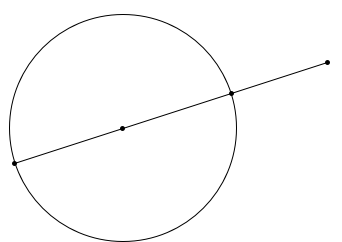
\includegraphics[width=0.4\textwidth]{assets/eddegree-circle.png}
  \caption{The ED degree of a line is one, of a circle two, of a parabola three and of an ellipsoid four.}
\end{figure}

\begin{cor}[ML Degree equals ED degree]
  The ML degree equals the ED degree for Gaussian models with unit covariance.
\end{cor}

\begin{cor}[Rationality of score equations for Gaussian models with unit covariance]
  The score equations for Gaussian models with identity covariance matrix are rational in \( \mu \).
\end{cor}

\begin{eg}[Nodal cubic]
  Assume \( \Theta_1 = \left\{ \begin{bmatrix}t^2 - 1\\ t(t^2 - 1)\end{bmatrix} \mid t \in \mathbb{R} \right\} \); this is a nodal cubic.
  \begin{figure}[H]
    \centering
    \includegraphics*[width=0.5\textwidth]{assets/nodal-cubic.jpg}
  \end{figure}
  Assume the covariance is fixed to be the identity matrix. Then the ML degree equals the ED degree; find \( \mu \in \mathbb{R}^2 \) in \( \Theta_1 \) such that it minimizes
  \begin{align*}
    \lVert \bar X - \mu \rVert^2 = (\bar X_1 - t^2 + 1)^2 + (\bar X_2 - t(t^2 - 1))^2.
  \end{align*}
  Computing the derivative yields 
  \begin{align*}
    &\frac{\partial}{\partial t} \left((\bar X_1 - t^2 + 1)^2 + (\bar X_2 - t(t^2 - 1))^2\right) \\&= 2(\bar X_1 - t^2 + 1) \cdot (-2t) + 2(\bar X_2 - t(t^2 - 1)) \cdot (-3t^2 + 1).
  \end{align*}
  Setting this to zero, we get a polynomial score equation in \( t \) of degree \( 5 \). The ED degree equals 5.
\end{eg}

\begin{mdframed}
\begin{prop}[Unrestricted mean and restricted covariance matrix]
  Let \( \Theta = \mathbb R^m \times \Theta_1 \), where \( \Theta_1 \subset \mathrm{PD}_m \). Then the maximum likelihood estimate is
  \begin{align*}
    \hat \mu = \bar X \quad \text{and} \quad \hat \Sigma = \mathrm{argmin}_{\Sigma \in \Theta_1} \log\det(\Sigma) + \mathrm{tr}(\Sigma^{-1}S).
  \end{align*}
  Alternatively, in terms of the precision matrix \( K = \Sigma^{-1} \), we have
  \begin{align*}
    \hat \mu = \bar X \quad \text{and} \quad \hat K = \mathrm{argmax}_{K \in \Theta_1^{-1}} \log\det(K) - \mathrm{tr}(KS).
  \end{align*}
\end{prop}
\end{mdframed}

\begin{prop}[Centered model and restricted covariance matrix]
  Another special case is given if we have a centered model, that is \( \Theta = \left\{ 0 \right\} \times \Theta_1 \). Then we have the same result as in the previous proposition but now with \( S = \frac{1}{N} \sum^N_{i=1}x^{(i)}{x^{(i)}}^T \).
\end{prop}

\begin{eg}[Full independence and centered model]
  Let \( \mathbf X = (X_1, X_2, X_3) \) be a random normal vector.
  Assume \( \Theta \) is centered and given by full independence \( X_1 \indep (X_2, X_3), X_2 \indep (X_1,X_3) \) and \( X_3 \indep (X_1,X_2) \). Then 
  \begin{align*}
    \Theta_1 = \left\{ \begin{bmatrix}
        \sigma_{11} & 0 & 0 \\
        0 & \sigma_{22} & 0 \\
        0 & 0 & \sigma_{33}
    \end{bmatrix}\right\} \subset \mathrm{PD}_3 \quad \text{and} \quad \Theta_1^{-1} = \left\{ 
    \begin{bmatrix}
      \frac{1}{\sigma_{11}} & 0 & 0 \\
      0 & \frac{1}{\sigma_{22}} & 0 \\
      0 & 0 & \frac{1}{\sigma_{33}}
    \end{bmatrix}
     \right\}  \subset \mathrm{PD}_3.
  \end{align*}
  Further, assume that we are given the sample covariance matrix
  \begin{align*}
    S = \begin{bmatrix}
      s_{11} & s_{12} & s_{13} \\
      s_{21} & s_{22} & s_{23} \\
      s_{31} & s_{32} & s_{33}
    \end{bmatrix}.
  \end{align*}
  Let \( a = \sigma_{11}^{-1} \), \( b = \sigma_{22}^{-1} \) and \( c = \sigma_{33}^{-1} \).
  The likelihood function if \( K \) is
  \begin{align*}
    \log \det K - \mathrm{tr}(KS) = \log(abc) - (s_{11}a + s_{22}b + s_{33}c ).
  \end{align*}
  Take the derivative with respect to \( a \), \( b \) and \( c \) and set to zero. We get that the ML degree is one and 
  \begin{align*}
    \hat \Sigma = \begin{bmatrix}
      s_{11} & 0 & 0 \\
      0 & s_{22} & 0 \\
      0 & 0 & s_{33}
    \end{bmatrix}.
  \end{align*}
\end{eg}

\begin{eg}[Bivariate centered model and restricted covariance matrix]
  Let \( \mathbf X =(X_1, X_2) \) be a random normal vector. Assume it is centered and 
  \begin{align*}
    \Theta_1 = \left\{ \begin{bmatrix}1 & \rho \\ \rho & 1\end{bmatrix} \mid \rho \in (-1,1) \right\}.
  \end{align*}
  The parameter \( \rho \) is the correlation between \( X_1 \) and \( X_2 \), i.e. \( \rho = \mathrm{Corr}(X_1, X_2) \). Assume we have sample covariance matrix 
  \begin{align*}
    S = \begin{bmatrix}
      s_{11} & s_{12} \\ s_{12} & s_{22}
    \end{bmatrix};
  \end{align*}
  note that this matrix is symmetric. Also, we compute the precision matrix 
  \begin{align*}
    \Sigma^{-1} = K = \frac{1}{1 - \rho^2} \begin{bmatrix}
      1 & - \rho \\ -\rho & 1
    \end{bmatrix}
  \end{align*}
  The log-likelihood is 
  \begin{align*}
    \ell_{\mathbf X}(\theta) \propto \log \det \Sigma + \mathrm{tr}(\Sigma^{-1}S) = \log(1 - \rho^2) + \frac{1}{1 - \rho^2} (s_{11} + s_{22} -2 \rho s_{12}).
  \end{align*}
  Take the derivative with respect to \( \rho \) and setting this to zero gives
  \begin{align*}
    \frac{\partial}{\partial\rho}  \ell_{\mathbf X}(\theta) \propto \frac{-2\rho}{ 1 - \rho^2} + \frac{-2s_{12}(1 - \rho^2) - (s_{11} + s_{22} - 2\rho s_{12}) \cdot (-2 \rho)}{(1 - \rho^2)^2} = 0.
  \end{align*}
  The score equation is 
  \begin{align*}
    \rho^3 - s_{12}\rho^2 + (s_{11} + s_{22} - 1)\rho - s_{12} = 0.
  \end{align*}
  The ML degree is three.
\end{eg}

\begin{eg}[Ungeneric data]
  Continuing the last example, suppose we have ``ungeneric'' data \( S \) with \( s_{12} = 0 \). Then, the score equation becomes
  \begin{align*}
    \rho(\rho^2 + s_{11} + s_{22} - 1)= 0.
  \end{align*}
  One MLE solution is \( \hat \rho = 0 \). If \( s_{11} + s_{22} > 1 \), then \( \hat \rho = 0 \) is the unique solution, and we have \( \hat \Sigma = \begin{bmatrix}
    1 & 0 \\ 0 & 1
  \end{bmatrix} \). For the other case \( s_{11} + s_{22} < 1 \), we get two further solutions on top of \( \hat \rho = 0 \); this is the generic case.
\end{eg}

\begin{eg}
  Assume a centered normal model and \( \Theta_1 = \left\{ \Sigma \in \mathrm{PD}_4 \mid \sigma_{12} = \sigma_{34} = 0 \right\} \); this means that \( X_1 \indep X_2 \) and \( X_3 \indep X_4 \). We have
  \begin{align*}
    \Sigma = \begin{bmatrix}
      \sigma_{11} & 0 & \sigma_{13} & \sigma_{14} \\
      0 & \sigma_{22} & \sigma_{23} & \sigma_{24} \\
      \sigma_{13} & \sigma_{23} & \sigma_{33} & 0 \\
      \sigma_{14} & \sigma_{24} & 0 & \sigma_{44}
    \end{bmatrix}
  \end{align*}
  Assume we observed this random (and generic) sample covariance matrix 
  \begin{align*}
    S = \begin{bmatrix}
      19 & 3 & 5 & 7 \\
      3 & 23 & 11 & 13 \\
      5 & 11 & 31 & -1 \\
      7 & 13 & -1 & 37
    \end{bmatrix};
  \end{align*}
  note that this matrix is positive definite. We want to use Macaulay2 to compute the critical solutions of 
  \begin{align*}
    \log \det \Sigma + \mathrm{tr}(\Sigma^{-1}S).
  \end{align*}
  To compute \( \Sigma^{-1} \) we use \(     \Sigma^{-1} = \frac{1}{\det \Sigma}\mathrm{adj}(\Sigma)
  \).
  If we compute the critical solutions of \(  \log \det \Sigma + \mathrm{tr}(\Sigma^{-1}S) \) with Macaulay2, we need to first turn the equations into a polynomial. Define \( f = \det \Sigma \) and \( L = \mathrm{tr}(\mathrm{adj}(\Sigma) S) \). Then the log-likelihood becomes
  \begin{align*}
    \ell = \log f + \frac{1}{f}L.
  \end{align*}
  So the score equations are
  \begin{align*}
   \frac{1}{f}\frac{\partial f}{\partial \sigma_{ij}} + \frac{\frac{\partial L}{\sigma_{ij}}f - L \frac{\partial f}{\sigma_{ij}}}{f^2} = 0.
  \end{align*}
  Multiply by \( f^2 \), and we get an ideal in the polynomial ring. Compute the vanishing set of the saturated ideal with respect to \( (f) \); we need the saturation to remove unwanted zeroes that were introduced by \( f \). Then, we see that the ML degree is 17.
\end{eg}


\subsection{Discrete models with constraints}

Let \( \mathcal{M} \subset \Delta_{r - 1} \) be a family of discrete models.

\begin{defi}[Likelihood function in projective space]
  Let \( V \subset \mathbb P^{r - 1} \) be an irreducible projective variety over \( \mathbb{C} \), and let \( \mathbf u \in \mathbb{N}^r \) be a vector of counts. The likelihood function \( L_\mathbf u: V \to \mathbb{C} \) is defined as
  \begin{align*}
    L_\mathbf u (\mathbf p) = \frac{p_{1}^{u_1} \dots p_r^{u_r}}{(p_1 + \dots + p_r)^{u_1 + \dots + u_r}}.
  \end{align*}
  Note that if \( \mathbf p \in \Delta_{r - 1} \), we recover the usual likelihood function. Moreover, \( L_\mathbf u  \) is a rational function in \( \mathbf p \) of degree zero (the numerator is of degree \( u_+ \) and the denominator has also degree \( u_+ \)).
\end{defi}

Previously, we assigned the ML degree to statistical models; now we assign the ML degree to projective varieties.

\begin{defi}[ML degree of projective varieties]
  The ML degree of \( V \) is the number of critical points \( \mathbf{p} \) of \( L_\mathbf u \) for generic \( \mathbf u \) on \( \mathbf{p} \in V_{\text{reg}} \setminus \mathcal{H} \) where \( \mathcal{H} = V(p_1...p_r(p_1 + ... + p_r)) \). 
\end{defi}

Since \( \mathbf p \) is constrained, we use Lagrange multipliers to find the critical points of \( L_\mathbf u \).

\begin{remark}[Lagrange multipliers]
  Assume \( V = (f_1, \dots, f_k) \). These are our \( k \) constraints.
  We optimize the log of \( L_\mathbf u \) plus the Lagrange multipliers:
  \begin{align*}
    \mathcal{L}_\mathbf u(\mathbf p, \lambda) = \left(\sum_{i=1}^r u_i \log(p_i)\right) - u_+\log(p_+) + \sum^k_{j=1} \lambda_j f_j.
  \end{align*}
  So, the score equations are 
  \begin{align*}
    \frac{\partial \mathcal{L}_\mathbf u}{\partial p_i}(\mathbf p)  &= \frac{u_i}{p_i} - \frac{u_+}{p_+} + \sum_{j=1}^k \lambda_j \frac{\partial f_j}{\partial p_i}(\mathbf p) = 0 \\
    \frac{\partial \mathcal{L}_\mathbf u}{\partial \lambda_j}(\mathbf p) &= f_j(\mathbf p) = 0.
  \end{align*}
\end{remark}

\begin{eg}[Binomial model with two trials]
  Let \( X \) be a discrete random variable. Assume \( V \) is given by \( p_1^2 - 4p_0p_2 \). Given counts \( \mathbf u = (u_0, u_1, u_2) \) find \( \theta \) such that \(\mathbf p_\theta \in V \) that maximizes \( L_\mathbf u \). Note that the implicit equation characterizes the binomial model with two trials. So in the end, we should end up with the ML estimator for the binomial model. Let's see if this is indeed the case.
  
  The Lagrange function is
  \begin{align*}
    \mathcal{L}_\mathbf u (\mathbf p, \lambda) = u_0 \log(p_0) + u_1 \log(p_1) + u_2 \log(p_2) - \lambda p_1^2 +  \lambda 4p_0p_2.
  \end{align*}
  We have 
  \begin{align*}
    \frac{\partial}{\partial p_0}: \frac{u_0}{p_0} - \frac{u_+}{p_+} + 4\lambda p_2 = 0 \\
    \dots
  \end{align*}
  Solve for \( p_0,p_1,p_2 \) and \( \lambda \) in terms of \( u_0, u_1 \) and \( u_2 \) gives 
  \begin{align*}
    \begin{bmatrix}
      \hat p_0 \\ \hat p_1 \\ \hat p_2
    \end{bmatrix} =
    \begin{bmatrix}
      \frac{(2u_0 + u_1)^2}{4(u_0 + u_1 + u_2)^2} \\
      \frac{(2u_0 + u_1)(u_1 + 2u_2)}{2(u_0 +  u_1 + u_2)^2} \\
      \frac{(u_1 + 2u_2)^2}{4(u_0 + u_1 + u_2)^2}
    \end{bmatrix}
  \end{align*}
  This is consistent with \( \mathrm{Bin}(2, \theta) \) where 
  \begin{align*}
    \hat \theta = \frac{u_1 + 2u_2}{2(u_0 + u_1 + u_2)}.
  \end{align*}
  Note that if by chance the count \( \mathbf u \) lies in \( V(p_1^2 - 4p_0p_2) \) then \( \lambda = 0 \) and \( \hat{\mathbf p} = \frac{1}{\mathbf u_+}(u_0,u_1,u_2)\).
\end{eg}

\begin{eg}[Independence model]
  Assume the statistical model 
  \begin{align*}
    \mathcal{M} = \left\{ \begin{bmatrix} p_{11} & p_{12} \\ p_{21} & p_{22} \end{bmatrix} \in \Delta_3 \mid p_{11}p_{22} - p_{12}p_{21} = 0 \right\} 
  \end{align*}
  What is this model? What is the MLE? We know that this is the independence model \( X \indep Y \) for \( X,Y \in [2] \). The MLE is given by 
  \begin{align*}
    \hat p_{ij} = \frac{u_{i+}u_{+j}}{u_{++}^2}.
  \end{align*}
  If we had computed critical solutions to the Lagrange equation we would have obtained the exact same result as above.
\end{eg}

June Huh proved in 2014 that if the ML degree of a variety is one, then  \( \hat{\mathbf p} \) is always a rational function in \( \mathbf u \) of degree zero where numerator and denominator are products of linear form.

\begin{defi}[Algebraic torus]
  The \textbf{algebraic torus} is \( (\mathbb{C}^*)^r = (\mathbb{C} \setminus \left\{ 0 \right\})^r \).
\end{defi}

\begin{defi}[Very affine variety]
  A \textbf{very affine variety} is a set of the form \( V \cap (\mathbb{C}^*)^r \) where \( V \subset \mathbb{C}^r \) is a variety.
\end{defi}

Our statistical model live in the probability simplex; from an algebraic geometry point of view, we consider our model to live in a very affine variety.

\begin{thm}[June Huh, 2014]
  Let \( X \) be a discrete random variable with state space \( \mathcal{X} = [r] \), and \( V \) a very affine variety.
  Let \( \mathrm{MLdegree}(V) = 1 \). Then, there exists \( \mathbf h  \in \mathbb{C}^r \) and a matrix \( \mathbf B \in \mathbb{Z}^{n \times r} \) where all columns sum to zero such that 
  \begin{align*}
    \hat p_j(u_1, \dots, u_r) = h_j \prod^n_{i=1}\left( \sum^r_{k=1} b_{ik} u_k \right)^{b_{ij}}
  \end{align*}
  \( (\mathbf B,\mathbf h) \) is called a \textbf{Horn pair}.
\end{thm}

\begin{eg}[Binomial model with two trials]
  Let \( \mathbf h = \begin{bmatrix}
    1 & 2 & 1
  \end{bmatrix} \) and \( \mathbf B = \begin{bmatrix}
    2 & 1 & 0 \\ 0 & 1 & 2 \\ -2 & -2 & -2
  \end{bmatrix} \). Then 
  \begin{align*}
    \hat p_0 &= (2u_0 + 1u_1)^2  (0u_0 + u_1 + 2u_2)^0  (-2u_0 - 2u_1 - 2u_2)^{-2}\\ &= \frac{(2u_0 + u_1)^2}{(-2u_0 - 2u_1 - 2u_2)^{2}}
  \end{align*}
  Similarly, 
  \begin{align*}
    \hat p_1 &= 2\left( (2u_0 + u_1) (u_1 + 2u_2) (-2u_0 - 2u_1 - 2u_2)^{-2} \right) \\
    \hat p_2 &= (2u_0 + u_1)^0 (u_1 + 2u_2)^{2} (-2u_0-2u_1-2u_2)^{-2}
  \end{align*}
\end{eg}

\begin{eg}[Independence model]
  Assume \( X \indep Y \), \( X,Y \in [2] \). We know \( \hat p_{ij} = \frac{p_{i+}p_{+j}}{p_{++}^2} \). What is \( \mathbf h \) and \( \mathbf B \)? We have 
  \begin{align*}
    \hat p_{11} = \frac{(u_{11} + u_{12})(u_{11} + u_{21})}{u_{++}^2} \\
    \hat p_{12} = \frac{(u_{11} + u_{12})(u_{12} + u_{22})}{u_{++}^2} \\
    \hat p_{21} = \frac{(u_{21} + u_{22})(u_{11} + u_{21})}{u_{++}^2} \\
    \hat p_{22} = \frac{(u_{21} + u_{22})(u_{12} + u_{22})}{u_{++}^2}.
  \end{align*}
  Then 
  \begin{align*}
    \mathbf h = \begin{bmatrix}
      4 & 4 & 4 & 4
    \end{bmatrix} \quad \text{and} \quad \mathbf B = \begin{bmatrix}
      1 & 1 & 0 & 0 \\ 0 & 0 & 1 & 1 \\  1 & 0 & 1 & 0 \\ 0 & 1 & 0 & 1 \\ -2 & -2 & -2 & -2
    \end{bmatrix}.
  \end{align*}
  Note that \( \mathbf{B} \) contains \( \mathbf{A} \) as a submatrix, where \( \mathbf{A} \) is the matrix from the log-linear model. 
\end{eg}

\begin{thm}[June Huh, Euler characteristic]
  Let \( V \subset (\mathbb{C}^*)^r \) be a very affine variety of dimension \( d \). If \( V \) is smooth (i.e. it contains no singular points), then \( \mathrm{MLdegree}(V) = (-1)^d \mathcal{X}(V) \), where \( \mathcal{X}(V) \) is the Euler characteristic of \( V \).
\end{thm}

\subsection{Log-affine linear models}
We now consider the MLE of log-affine linear models.

\begin{mdframed}  
\begin{thm}[Birch's Theorem]
  Let \( \mathcal{M} \)  be a \emph{discrete} regular exponential family.
  Let \( A \in \mathbb{Z}^{k \times r} \) such that \( \mathbf{1} \in \mathrm{rowspan}(A) \), \( \mathbf h \in \mathbb{R}^r_{> 0} \) and \( \mathbf{u} \) vector of counts from \( N \) i.i.d. samples. Then the MLE, if it exists, is the unique solution to the equation 
  \begin{align*}
    A \mathbf{\bar u} = A \mathbf p
  \end{align*}
  with \( \bar{\mathbf u} = \frac{1}{N}\mathbf u \) is the empirical distribution and \( \mathbf p \in \mathcal{M}_{A,h} \). Note that if we do not restrict \( \mathbf p \) to lie in the probability simplex, then there may exist multiple solutions;.
\end{thm}
\end{mdframed}

\begin{proof}
  This follows from Corollary \ref{mle-discrete-regular-exp}, which concerned regular, not necessarily discrete, exponential families. Note that \( \mathbf u \) is always a sufficient statistic for a discrete model. \( A \mathbf u \) is the minimal sufficient statistic for a log-linear model.

  Let \( \mathbf X = (X^{(1)}, \dots, X^{(N)}) \) be an i.i.d. sample with state space \( \mathcal{X} = [r]^{N} \). Then, 
  \begin{align*}
    T(\mathbf X) = \sum_{i=1}^N T(X^{(i)}).
  \end{align*}
  Recall that for log-affine linear models, the columns \( \mathbf a_{\cdot j} \) of \( A \) consists of \( T(1), \dots , T(r) \). So, we get
  \begin{align*}
    T(\mathbf X) =  \sum^r_{i=1} u_i T(j) = \sum^r_{i=1} u_i \mathbf a_{\cdot i} = A \mathbf u.
  \end{align*}
  Next, note that 
  \begin{align*}
    \mathbb{E}[T(X)] = N \cdot \mathbb{E}[T(X^{(N)})] = N \sum^r_{i=1} p_i T(i) = N A \mathbf p.
  \end{align*}
  Hence, \(     N A \mathbf p = \mathbb{E}[T(X)] = T(X) = A \mathbf u
  \).
\end{proof}

Let \( A = \begin{bmatrix}
 \vline & \dots & \vline \\
 \mathbf a_{\cdot 1} & \dots & \mathbf a_{\cdot r} \\
  \vline & \dots & \vline
\end{bmatrix} \in \mathbb{Z}^{k \times r} \) such that \( \mathbf{1} \in \mathrm{rowspan}(A) \). Let \( \mathbf h \in \mathbb{R}^r_{> 0} \). We can define a lattice polytope by \( P(A) = \mathrm{conv}\left\{ a_1, \dots, a_r \right\} \subset \mathbb{R}^k \). A point \( p \) lies in the relative interior of a polytope \( P = \mathrm{conv}\left\{ p_i \right\} \) if there exists a positive convex combination of the vertices that equals \( p \); note that not every convex combination for \( p \) need be positive.

\begin{mdframed}
\begin{thm}[Existence of MLE]
  Let \( \mathcal{M}_{A, \mathbf h} \) be a discrete exponential family. The MLE exists for \( \mathcal{M}_{A, \mathbf{h}} \) if and only if \( A \bar{\mathbf u}  \in \mathrm{relint}(P(A))\).
\end{thm}
\end{mdframed}

\begin{proof}
  \( \implies \):
  Assume the MLE exists for \( \mathcal{M}_{A, \mathbf h} \). By Birch's Theorem there exists a \( \mathbf p \in \mathcal{M}_{A, \mathbf h} \) such that \( A \mathbf p = A \mathbf{\bar u} \). Recall that \(\mathbf  p \in \mathcal{M}_{A, \mathbf{h}} \) means that \( \mathbf p \) lies in the interior of the probability simplex. Hence, \( A \mathbf{\bar u} \) lies in the relative interior of \( P(A) \) since all \( p_i > 0 \) for \( i = 1, \dots, r \).

  If \( \mathbf b = A \mathbf{\bar u} \in \mathrm{relint}(A) \), then there exists positive \( \mathbf v \in \mathbb{R}^r_{> 0} \) such that \( N\mathbf b = A \mathbf{v} \). Observe that the likelihood \( \prod p_i^{u_i} \) can be replaced by \( \prod p_i^{v_i} \) since \( A \mathbf u = A \mathbf{v} \). Next, note that on the boundary of \( \mathbf{p} \in \mathcal{M}_{A, \mathbf{h}} \), the likelihood is zero because all exponents \( v_i > 0 \) and some \( p_i =0 \). Note that in the interior of \( \mathcal{M}_{A, \mathbf{h}} \) the likelihood is positive. Since the likelihood function of an exponential family is concave, a maximum is attained in the interior of \( \mathcal{M}_{A, \mathbf{h}} \).
\end{proof}

There are only two cases: if \( \bar{\mathbf u} \) lies on the boundary of \( P(A) \), then the MLE does not exist. If \( \bar{\mathbf u} \) lies in the relative interior of \( P(A) \), then the MLE exists and is unique.

\begin{cor}
  If all the components of \( \mathbf u \) are positive, then the MLE exists and is unique.
\end{cor}

\begin{eg}[Independence model]
  Consider \( \mathcal{M}_{X \indep Y} \) with \( X,Y \in [2] \). Does the MLE exist? For which data does it exist?
   
  \( \mathcal{M}_{X \indep Y} \) is a log-linear model with 
  \begin{align*}
    A = \begin{bmatrix}
      \vline & \vline & \vline & \vline \\
      \mathbf a_{\cdot 1} &  \mathbf a_{\cdot 2} &  \mathbf a_{\cdot 3} &  \mathbf a_{\cdot 4} \\
      \vline & \vline & \vline & \vline 
    \end{bmatrix} = \begin{bmatrix}
      1 & 1 & 0 & 0 \\
      0 & 0 & 1 &1 \\
      1 & 0 & 1 & 0 \\
      0 & 1 & 0 & 1 
    \end{bmatrix}.
  \end{align*}

  The polytope \( P(A) \subset \mathbb{R}^4 \) lives in \( \mathbb{R}^2 \). Assume we are given some data \( \mathbf u  \in \mathbb{N}^4\). If all \( u_i > 0 \), then the MLE exists. If some \( u_i =0 \), then it can go wrong.

  \begin{itemize}
    \item Let \( \mathbf u = (2,0,0,3) \). Then 
    \begin{align*}
      A \bar{\mathbf{u}} = \frac{1}{5}(2 \cdot \mathbf{a}_{\cdot 1} + 3 \cdot \mathbf{a}_{\cdot 4}) = \frac{1}{5}\begin{bmatrix}
        2 \\ 3 \\ 2 \\ 3
      \end{bmatrix}
    \end{align*}
    The point \( \frac{1}{5}\begin{bmatrix}
      2 & 3 & 2 & 3
    \end{bmatrix}^T \) lives in the relative interior of \( P(A) \) since we can find a positive convex combination of vertices of \( A \) such that 
    \begin{align*}
      \frac{1}{5}\begin{bmatrix}
        2 \\ 3 \\ 2 \\ 3
      \end{bmatrix} = A \begin{bmatrix}
        1 \\ 1 \\ 1 \\ 2
      \end{bmatrix}.
    \end{align*}

    \item Let \( \mathbf{u} = (1,0,1,0) \). Then \( A\bar{\mathbf{u}} = \frac{1}{2}(1,1,2,0) \). This lives on the boundary of the polyope; hence no MLE exists.
  \end{itemize}
\end{eg}

\subsection{Gaussian linear concentration models}

Let \( L \subset \mathbb{R}^{\frac{m(m+1)}{2}} \) be a linear space of matrices such that \( L \cap \mathrm{PD}_m \neq \emptyset \).
Recall the Gaussian linear concentration model \( \mathcal{M}_L \); this model consists of all normal distributions in \( \mathcal{N}(\cdot, \Sigma) \)  parametrized by \( \Sigma \in L^{-1} = \left\{ \Sigma \in \mathrm{PD}_m \mid \Sigma^{-1} \in L \right\} \). The likelihood is given by 
\begin{align*}
  \ell_K(S) = \log \det K - \mathrm{tr}(KS).
\end{align*}
A minimal sufficient statistic is \( T(X) = \pi_L(S) \), the orthogonal projection of the sample covariance matrix \( S \) onto the linear space \( L \).

\begin{thm}[MLE estimator for Gaussian linear concentration models]
  Let \( \Theta = \mathbb{R}^m \times L^{-1} \) be the parameter space of \( \mathcal{M}_L \). Let \( X^{(1)}, \dots, X^{(N)} \in \mathbb{R}^m \) i.i.d. sample. Then the MLE for \( (\mu, \Sigma) \in \Theta \), if it exists, is \( (\bar X, \hat \Sigma) \) where \( \hat \Sigma \) is the unique solution to 
  \begin{align*}
    \pi_L(\hat \Sigma) = \pi_L(S), \quad \hat \Sigma \in L^{-1}.
  \end{align*}
\end{thm}

\begin{prop}[Existence of MLE for Gaussian linear concentration models]
  The MLE exists for Gaussian linear concentration models if and only if \( \pi^{-1}_L(S) \neq \emptyset   \) if and only if \( \pi_L(S) \in \mathrm{relint(\mathcal{C}_L)} \); here \( \mathcal{C}_L \) denotes the cone of matrices in \( L \).
\end{prop}

\begin{eg}[Gaussian graphical models]
  The linear space \( L \) can be given by a Gaussian graphical model \( G \). It consists of matrices  
  \begin{align*}
    L = \left\{ (k_{ij})_{i,j}  \mid k_{ij} = 0 \iff \text{there is no edge between \( i \) and \( j \) in \( G \)}  \right\}.
  \end{align*}
  For instance, consider the following Gaussian graphical model 
  \begin{figure}[H]
    \centering
    % https://tikzcd.yichuanshen.de/#N4Igdg9gJgpgziAXAbVABwnAlgFyxMJZABgBpiBdUkANwEMAbAVxiRAEYQBfU9TXfIRTtyVWoxZsATN14gM2PASJl2Y+s1aIQAZll9FgoiLXUNk7QBZuYmFADm8IqABmAJwgBbJGRA4ISCIgABYwdFBskGCsPK4e3ohB-kg61KHhkQQxcu5eSFLUyYipIWER2lHZcXmIvkUFpRkVWTZcQA
\begin{tikzcd}
  1 \arrow[r, no head] \arrow[d, no head] & 2 \arrow[d, no head] \\
  3 \arrow[r, no head]                    & 4                   
  \end{tikzcd}
  \end{figure}
  There is no edge between \( (2,3)  \)  and \( (1,4) \); so \( L \) consists of matrices 
  \begin{align*}
    L = \left\{ \begin{bmatrix}* & * & * & 0 \\ * & * & 0 & * \\ * & 0 & * & * \\ 0 & * & * & *\end{bmatrix} \right\}.
  \end{align*}
\end{eg}

\begin{thm}[MLE for Gaussian graphical models]
  Let \( G \) be an undirected graph. The MLE estimator \( (\hat \mu, \hat \Sigma) \) of the Gaussian graphical model \( \mathcal{M}_G \) given sufficient statistic \( T(X) = (\bar X, S) \) is 
  \begin{align*}
    \bar \mu = \bar X \quad \text{and} \quad \hat \Sigma_{ij} = s_{ij}\; \text{if \( i \leftrightarrow j \in G \) or \( i=j \)}, \quad  \hat \Sigma^{-1}_{ij} =0 \; \text{if \( i \leftrightarrow j \notin G \)}
  \end{align*}
  provided the MLE exists. In words, whenever there is an edge between \( i \) and \( j \) in \( G \), we set \( \hat \Sigma_{ij} = s_{ij} \); when there is no edge, the \( (i,j) \)-th component of \( \hat \Sigma \) is only implicitly given by the inverse.
\end{thm}

\begin{eg}
  Consider the following Gaussian graphical model \( G \):
  \begin{figure}[H]
    \centering 
    % https://tikzcd.yichuanshen.de/#N4Igdg9gJgpgziAXAbVABwnAlgFyxMJZABgBpiBdUkANwEMAbAVxiRAEYQBfU9TXfIRTtS7KrUYs2AZm68QGbHgJEATOXH1mrRCFXdxMKAHN4RUADMAThAC2SESBwQk6kAAsYdKG0hhWPJY29oiOzkhkHl4+un4BFFxAA
\begin{tikzcd}
  1 &                                           & 2 \\
    & 3 \arrow[ru, no head] \arrow[lu, no head] &  
  \end{tikzcd}
  \end{figure}
  The linear space is 
  \begin{align*}
    L = \left\{ \begin{bmatrix}* & 0 & * \\ 0 & * & * \\ * & * & *\end{bmatrix} \right\}.
  \end{align*}
  What is \( \hat \Sigma \) of the graphical model \( \mathcal{M}_G \)? Assume we have data \( S \). Then, we know by the above theorem that 
  \begin{align*}
    \hat \Sigma = \begin{bmatrix}
      s_{11} &x & s_{13} \\
      x & s_{22} & s_{23} \\
      s_{13} & s_{23} & s_{33}
    \end{bmatrix}.
  \end{align*}
  The entry \( \hat \Sigma_{12} \) must be chosen in a way such that \( \hat \Sigma_{12}^{-1} = 0 \); using the formula \( \hat \Sigma^{-1}_{ij} = (-1)^{i+j} \frac{1}{\det \hat \Sigma} \mathrm{det}(\hat \Sigma_{ji}) \), we obtain 
  \begin{align*}
    \hat \Sigma^{-1}_{12} = (-1)^{1 + 2}\frac{1}{\det \hat \Sigma}(x s_{33} - s_{13}s_{23}) =0.
  \end{align*}
  So \( x =  \frac{s_{13}s_{23}}{s_{33}}\).
\end{eg}

\clearpage
\section{Fisher's exact test}

\subsection{Asymptotic test}

\textbf{Question:} Is the true generating distribution \( \mathbf p\in \Delta_{rc - 1} \) really part of \( \mathcal{M}_{X \indep Y} \)?

We define 
\begin{itemize}
  \item \( H_0 \): \( X  \indep Y\)
  \item \( H_1 \): \( X \) and \( Y \) are no independent
\end{itemize}

\begin{defi}[Chi-Square-statistic]
  It is defined by 
  \begin{align*}
    \chi^2(\mathbf u) = \sum^r_{i=1} \sum^c_{j=1} \frac{(u_{ij} - e_{ij})^2}{e_{ij}}
  \end{align*}
  where \( e_{ij} = \frac{u_{i+} u_{+j}}{u_{++}} \) is the expected count.
\end{defi}

\begin{remark}
  If \( X \) and \( Y \) were independent, then we would expect \( (u_{ij} - e_{ij})^2 \) to be small.
\end{remark}

\begin{mdframed}
  \textbf{Decision rule: }
If \( \chi^2(\mathbf u) \) is small, we keep \( H_0 \). If \( \chi^2(\mathbf u) \) is large, we reject \( H_0 \).
\end{mdframed}

\begin{proof}[Reasoning]
 Suppose now, \( (u_{ij} - e_{ij})^2 \) is large. What does that mean? Either, \( X \) and \( Y \) are independent, but our estimate is bad, or \( X \) and \( Y \) are dependent. Since the estimator is optimal, we infer that \( X \) and \( Y \) are dependent.
\end{proof}


\begin{defi}[p-value]
  The \( p \)\textbf{-value} of the \( \chi^2 \)-test is the probability under \( H_0 \) to observe an equal or greater value of \( \chi^2 \) than the observed one \( \chi^2(\mathbf u) \).
\end{defi}

How do we compute this \( p \)-value? We can approximate it with the following theorem.

\begin{thm}
  Let \( X \in [r] \) and \( Y \in [c] \). Let \( \mathbf p \in \mathcal{M}_{X \indep Y} \subset \Delta_{rc - 1}\) be the true joint distribution. If \( \mathbf u_N \) is a contingency table with sample size \( N \), then 
  \begin{align*}
    \chi^2(\mathbf u_N) \overset{\text{distribution}}{\to} \chi^2_{(r-1)(c-1)}
  \end{align*}
  as \( N \to \infty \). We call the \( \chi^2_{(r-1)(c-1)} \) the \emph{Chi-squared distribution} with \( (r-1)(c-1) \) degrees of freedom. It is the distribution of \( \sum_{i=1}^{(r-1)(c-1)} z_i^2 \) where all \( z_i \sim \mathcal{N}(0,1) \) i.i.d. Note that this distribution does not depend on the true distribution \( \mathbf p \).
\end{thm}

Recall that convergence in distribution means 
\begin{align*}
  \lim_{N \to \infty} \mathbb{P}(\chi^2(\mathbf u_N) \geq t) = \mathbb{P}(\chi^2_{(r-1)(c-1)} \geq t) \quad \forall t.
\end{align*}
Hence, to compute the \( p \)-value, that is to compute 
\begin{align*}
  \mathbb{P}(\chi^2(U) \geq \chi^2(\mathbf u)),
\end{align*}
we can instead compute the \textbf{asymptotic \( p \)-value}
\begin{align*}
  \mathbb{P}(\chi^2_{(r-1)(c-1)} \geq \chi^2(\mathbf u)) .
\end{align*}

\begin{eg}[Glasses and handedness]
  Assume \( X,Y \in \left\{ 0,1 \right\} \) and
  \begin{align*}
    X \,&...\, \text{wears glasses if \( X = 1 \)}, \\
    Y \, &...\, \text{handedness if \( Y = 1 \)}.
  \end{align*}
  Let \( N = 100 \). Assume we have the following contingency table.
  \begin{table}[H]
    \centering
    \begin{tabular}{l|ll|ll}
    $X \ Y$ & right & left & $\mathbf u_{\cdot +}$  \\ \cline{1-4}
       glasses     & 43    & 9    & 52             \\
        no glasses    & 44    & 4    & 48             \\ \cline{1-4}
       \( \mathbf u_{+ \cdot} \)     & \( 87 \)    & \( 13 \)   &       \( 100 \)        
    \end{tabular}
  \end{table}
  We assert \( H_0: p \in \mathcal{M}_{X \indep Y} \) and \( H_1 : p \notin \mathcal{M}_{X \indep Y} \). Can we reject \( H_0 \)? Let's say our confidence interval is \( 1 - 0.05 = 95\% \).

  We compute the expected counts.
  \begin{align*}
    \hat p_{11} &= \frac{52 \cdot 87}{100 \cdot 100}\\
    \hat e_{11} &= \frac{52 \cdot 87}{100} = 45.24 \\
    \hat e_{12} &= \frac{52 \cdot 13}{100} = 6.76 \\
    \hat e_{21} &= \frac{48 \cdot 13}{100} = 41.76 \\
    \hat e_{22} &= \frac{48 \cdot 13}{100} = 6.24 \\
  \end{align*}
  Then 
  \begin{align*}
    \chi^2(\mathbf u) = \frac{(45.24 - 43)^2}{45.24} + \frac{(6.76 - 9)^2}{6.76} + \frac{(41.76 - 44)^2}{41.76} + \frac{(6.24 - 4)^2}{6.24} \approx 1.7774.
  \end{align*}
  Is this a high or a low \( \chi^2 \) value? To answer this we compute the asymptotic \( p \)-value
  \begin{align*}
    \mathbb{P}(\chi_{1}^2 \geq 1.7774) \approx 0.1825 > 0.05.
  \end{align*}
  We do not reject \( H_0 \), in other words handedness and wearing glasses are independent.
\end{eg}

\textbf{Problem:} Can we trust this asymptotic approximation? What if \( N \) is small? 

The rescue is Fisher's exact test (1934).

\subsection{Independence model}

Let \( X \in [r] \) and \( Y \in [c] \). Assume \( \mathbf p \in \Delta_{rc - 1} \) is the joint distribution of \( X \) and \( Y \).
Consider a set of tables of size \( N \)
\begin{align*}
  T(N) = \left\{ \mathbf u \in \mathbb{N}^{r \times c} \mid u_{++} = N \right\}.
\end{align*}
Let \( U \in T(N) \) be a random variable. 

\textbf{Question:} What is the probability of observing a contingency table \( \mathbf u \)?
\begin{prop}
  It holds \( U \sim \mathrm{Multinomial}(N,\mathbf p) \), i.e.
  \begin{align*}
    \mathbb{P}(U = \mathbf u) = {N \choose u_{11}u_{12}...u_{rc}} \prod^r_{i=1} \prod^c_{j=1} p_{ij}^{u_{ij}} \quad \forall \mathbf{u} \in T(N).
  \end{align*}
  Here \( {N \choose u_{11}u_{12}...u_{rc}} = \frac{N!}{u_{11}!u_{12}! \dots u_{rc}!} \).
\end{prop}
\textbf{Problem: }This distribution depends on the true joint distribution \( \mathbf p \).

Fisher's idea was to restrict to tables with the same row and column sums as the observed data \( \mathbf u \). \emph{What is the probability to observe \( \mathbf u \) among all tables with the same row and column sum as \( \mathbf u \)?}

\begin{defi}[Hypergeometric distribution]
  The \textbf{hypergeometric distribution} \( X \sim \mathrm{HypGeo}(N, K, n) \) is defined as 
  \begin{align*}
    \mathbb{P}(X = k) = \frac{{K \choose k} {N - K \choose n - k}}{{N \choose n}}
  \end{align*}
  for \( \max\left\{ 0, n - (N - K) \right\} \leq k \leq
   \min\left\{ K, n \right\} \).
\end{defi}

We specialize to the case \( r=c=2 \) before considering general \( r \) and \( c \).

\begin{mdframed}
\begin{prop}[Conditional distribution of observing a contingengy table  for the independence model]
  Let \( r = c= 2 \) and \( \mathbf{p} \in \mathcal{M}_{X \indep Y} \). Assume \( \mathbf{u} \in T(N) \). Then 
  \begin{align*}
    \left(U \mid U_{1+} = \mathbf{u}_{1+}, U_{+1} = \mathbf{u}_{+1}\right) \sim \mathrm{HypGeo}(N, \mathbf{u}_{1+}, \mathbf{u}_{+1}).
  \end{align*}
  That means 
  \begin{align*}
    \mathbb{P}(U_{11} = u_{11} \mid U_{1+} = \mathbf{u}_{1+}, U_{+1} = \mathbf{u}_{1+}) = \frac{{\mathbf{u}_{1+} \choose u_{11}} {N - \mathbf{u}_{1+} \choose \mathbf u_{+1} - u_{11}}}{{N \choose \mathbf{u}_{+1}}}.
  \end{align*}
\end{prop}
\end{mdframed}

\begin{remark}
  Note that \( U_{11} = u_{11} \) given \( U_{1+} = \mathbf{u}_{1+}, U_{+1} = \mathbf{u}_{1+} \) uniquely determines the contingency table since \( \mathbf{u}_{2+} = N - \mathbf{u}_{1+} \) and \( \mathbf{u}_{+2} = N - \mathbf{u}_{+1} \).
\end{remark}

\begin{remark}
  Note that this conditional distribution \(  \mathrm{HypGeo}(N, \mathbf{u}_{1+}, \mathbf{u}_{+1}) \) does not depend on \( \mathbf{p} \).
\end{remark}

\clearpage
\begin{mdframed}
\begin{defi}[Conditional exact \( p \)-value of observing a contingency table]
  The \textbf{conditional exact \( p \)-value} is defined as 
  \begin{align*}
    \mathbb{P}(\chi^2(U) \geq\chi^2(u) \mid U_{1+} = \mathbf{u}_{1+}, U_{+1} = \mathbf{u}_{+1}).
  \end{align*}
\end{defi}
\end{mdframed}

\begin{eg}[The tea test]
  Assume \( X,Y \in \left\{ \text{Milk},\text{Tea} \right\} \) and
  \begin{align*}
    X \,&...\, \text{ingredient added first (ground truth)}, \\
    Y \, &...\, \text{ingredient added first according to colleague}.
  \end{align*}
  \begin{table}[H]
    \centering
    \begin{tabular}{l|ll|ll}
    $X \ Y$ & Milk & Tea & $\mathbf u_{\cdot +}$  \\ \cline{1-4}
       Milk     & 3    & 1    & 4             \\
        Tea    & 1    & 3    & 4             \\ \cline{1-4}
       \( \mathbf u_{+ \cdot} \)     & \( 4 \)    & \( 4 \)   &       \( 8 \)        
    \end{tabular}
  \end{table}
  As usual \( H_0: \mathbf{p} \in \mathcal{M}_{X \indep Y} \). If \( H_0 \) is true, then the colleague is just guessing.

  Computation of the expected count yields \( \mathbf e = \begin{bmatrix}
    2 & 2 \\ 2 & 2
  \end{bmatrix} \). Then, 
  \begin{align*}
    \chi^2(\mathbf u) = \frac{(3-2)^2}{2} + \frac{(1-2)^2}{2} + \frac{(1-2)^2}{2} + \frac{(3-2)^2}{2} = 2.
  \end{align*}
  Now we want to compute \( \mathbb{P}(\chi^2(U) \geq 2 \mid U_{1+} = 4, U_{+1} = 4) \). For \( u_{11} = 0 \) we obtain 
  \begin{align*}
    \mathbb{P}(U_{11} = 0 \mid  U_{1+} = 4, U_{+1} = 4) = \frac{{4 \choose 0} {4 \choose 4}}{{8 \choose 4}} = \frac{1}{70} \approx 0.014.
  \end{align*}
  Moreover, 
  \begin{align*}
    \chi^2(\mathbf u) = \frac{(0-2)^2}{2} + \frac{(4-2)^2}{2} + \frac{(4-2)^2}{2} + \frac{(0-2)^2}{2} = 8.
  \end{align*}
  Further computation of \( u_{11} \in \left\{ 1,2,3,4 \right\} \)
  gives 
  \begin{table}[H]
    \centering
    \begin{tabular}{l|ll}
    $u_{11}$ & \( \mathbb{P}(U_{11} = u_{11}) \) & \( \chi^2(\mathbf u) \) \\ \hline
    0        & 0.014 & 8    \\
    1        & 0.229 & 2    \\
    2        & 0.514 & 0    \\
    3        & 0.229 & 2    \\
    4        & 0.014 & 8   
    \end{tabular}
    \end{table}
  Hence, 
  \begin{align*}
    \mathbb{P}(\chi^2(U) \geq 2 \mid  U_{1+} = 4, U_{+1} = 4) = 0.486.
  \end{align*}
\end{eg}

We generalize to arbitrary \( r,c \in \mathbb{N} \).

\begin{defi}[Multivariate hypergeometric distribution]
  Let \( \mathbf{X} =(X_i)_{i=1,\dots, k} \) be a random vector. Let \( M_1, \dots, M_k, M, n \in \mathbb{N} \) such that \( n \leq M = \sum_{i=1}^k M_i \). Then \( \mathbf{X} \sim \mathrm{MultiHypGeom}(M_1, \dots, M_k, n) \) if the probability mass function is 
  \begin{align*}
    p_\mathbf X(\mathbf{x}) = p_\mathbf X(x_1, \dots, x_k) = \frac{\prod^k_{i=1} {M_i \choose x_i}}{{M \choose n}},  \quad \forall  \mathbf x \in \mathbb{N}^k: \sum_{i=1}^k  x_i = n.
  \end{align*}
  \( M_i \) denotes the subpopulation of class \( i \). The total population is \( M = \sum^k_{i=1} M_i \).
\end{defi}

\begin{remark}
  Note that \( \sum_{i=1}^k {M_i \choose x_i} = {M \choose n} \).
\end{remark}

\begin{prop}[How many ways exist to obtain a column of a contingengy table?]
  Let \( j \in [c] \). Let \(  u_{+j} \) be fixed. The number of ways of obtaining columns with counts \( \begin{bmatrix}
    u_{1j} & u_{2j} & \dots & u_{rj}
  \end{bmatrix}^T \) 
  is 
  \begin{align*}
    {u_{+j} \choose u_{1j}u_{2j} \dots u_{rj}}.
  \end{align*}
  Moreover, the number of ways of ordering the class sizes is 
  \begin{align*}
    {N \choose u_{1+} u_{2+} ... u_{r+}}.
  \end{align*}
\end{prop}

\begin{mdframed}  
\begin{thm}[Conditional distribution of observing contingency table for the independence model (general case)]
  Let \( \mathbf p \in \mathcal{M}_{X \indep Y} \). Fix some data \( \mathbf{u} \in T(N) \). Given marginal counts \( u_{+\cdot} \) and \( u_{\cdot +} \), it holds 
  \begin{align*}
    \mathbb{P}(U = \mathbf u \mid U_{+\cdot} = u_{+ \cdot}, U_{\cdot+} = u_{\cdot +}) = \frac{{u_{+1} \choose u_{11}u_{21} \dots u_{r1}} \dots {u_{+c} \choose u_{1c}u_{2c} \dots u_{rc}}}{{N \choose u_{1+}\dots u_{r+}}}.
  \end{align*}
  Using a more compact notation we write 
  \begin{align*}
    \mathbb{P}(U = \mathbf u \mid U_{+\cdot} = u_{+ \cdot}, U_{\cdot+} = u_{\cdot +}) = \frac{{u_{+1} \choose \mathbf{u}_{\cdot 1}} \dots {u_{+c} \choose \mathbf{u}_{\cdot c}}}{{N \choose \mathbf{u}_{\cdot +}}}.
  \end{align*}
\end{thm}
\end{mdframed}

\begin{mdframed}  
\begin{defi}[Exact \( p \)-value]
  The exact \( p \)-value is defined as
  \begin{align*}
    \mathbb{P}(\chi^2(U) \geq \chi^2(\mathbf u) \mid U_{\cdot +} = u_{\cdot +}, U_{+\cdot} = u_{+ \cdot}).
  \end{align*}
\end{defi}
\end{mdframed}

\begin{prop}[Explicit formula for the exact \( p \)-value]
  The explicit formula for the exact \( p \)-value is 
  \begin{align*}
    \mathbb{P}(\chi^2(U) \geq \chi^2(\mathbf u) \mid U_{\cdot +} = u_{\cdot +}, U_{+\cdot} = u_{+ \cdot}) = \frac{\sum_{\mathbf v} \left(\mathbbm{1}_{\chi^2(\mathbf v) \geq \chi^2(\mathbf u)} \cdot \frac{1}{\prod^r_{i=1} \prod^c_{j=1} v_{ij}!}\right)}{\sum_{\mathbf v} \frac{1}{\prod^r_{i=1} \prod^c_{j=1} v_{ij}!}},
  \end{align*}
  where we sum \( \mathbf{v} \) over \( T(\mathbf u_{\cdot+}, \mathbf u_{+\cdot}) = \left\{ \mathbf w \in T(N) \mid \mathbf{w}_{\cdot+} = \mathbf{u}_{\cdot +}, \mathbf{w}_{+\cdot} = \mathbf{u}_{+\cdot} \right\} \).
\end{prop}

% \begin{proof}
%   Start with 
%   \begin{align*}
%     &\mathbb{P}(\chi^2(U) \geq \chi^2(\mathbf u) \mid U_{\cdot +} = u_{\cdot +}, U_{+\cdot} = u_{+ \cdot}) \\
%     &= \sum_{\mathbf{v} \in T(\mathbf u_{\cdot+}, \mathbf u_{+\cdot})} \mathbbm{1}_{\chi^2(\mathbf{v}) \geq \chi^2(\mathbf{u})} \cdot \mathbb{P}(U = \mathbf v \mid U_{+\cdot} = u_{+ \cdot}, U_{\cdot+} = u_{\cdot +})
%   \end{align*}
%   We have 
%   \begin{align*}
%     \mathbb{P}(U = \mathbf v \mid U_{+\cdot} = u_{+ \cdot}, U_{\cdot+} = u_{\cdot +}) 
%     = \frac{{u_{+1} \choose \mathbf{v}_{\cdot 1}} \dots {u_{+c} \choose \mathbf{v}_{\cdot c}}}{{N \choose \mathbf{u}_{\cdot +}}}
%      = \frac{}{\sum }.
%   \end{align*}
% \end{proof}

\subsection{Log-affine linear models}

We generalize to log-affine linear models \( \mathcal{M}_{A, \mathbf{h}} \subset \Delta_{r-1} \). Assume we collect data \( X^{(1)}, \dots, X^{(n)} \in [r] \) i.i.d. according to some \( \mathbf{p} \in \mathrm{int}(\mathcal{M}_{A, \mathbf{h}}) \). We want to test 
\begin{align*}
  H_0: \mathbf{p} \in \mathcal{M}_{A, \mathbf{h}} \quad \text{versus} \quad H_1: \mathbf{p} \notin \mathcal{M}_{A, \mathbf{h}}.
\end{align*}
If the true distribution is indeed in \( \mathcal{M}_{A, \mathbf{h}} \), then we can write 
\begin{align*}
  \mathbf{p}_j = \frac{1}{Z(\theta)} h_j \theta^{\mathbf{a}_{\cdot j}}
\end{align*}
for some positive vector \( \mathbf{h} \in \mathbb{R}^r \), \( \theta = (\theta_1, \dots, \theta_k) \) and \( A \in \mathbb{Z}^{k \times r} \). The probability of observing a contingency table \( \mathbf{u} \) is given by 
\begin{align*}
  L(\mathbf u \mid \theta) = \frac{1}{Z(\theta)^n} {n \choose \mathbf{u}} \mathbf h^{\mathbf{u}} \theta^{A \mathbf{u}}.
\end{align*}
We define the fiber of a table \( \mathbf u \) to be the set of all tables \( \mathbf v \) that have the same sufficient statistic as \( \mathbf{u} \).
\begin{defi}[Fiber of a contingency table]
  Let \( \mathbf{u} \in \mathbb{N}^r \). The \textbf{fiber} is defined as 
  \( \mathcal{F}(\mathbf{u}) = \left\{ \mathbf{v} \in \mathbb{N}^r \mid A \mathbf{v} = A \mathbf{u} \right\} \).
\end{defi}
\begin{prop}[Conditional probability is independent on \( \theta \)]
  We have \(   L(\mathbf{v} \mid \mathbf{v} \in \mathcal{F}(\mathbf{u}), \theta) = \mathbb{P}(U = \mathbf{v} \mid v \in \mathcal{F}(\mathbf{u}))\).
\end{prop}
\begin{proof}
  The key idea is that the conditional probability \( L(\mathbf v \mid v \in \mathcal{F}(\mathbf{u}), \theta) \) does not depend on \( \theta \) since we have 
\begin{align*}
  L(\mathbf{v} \mid \mathbf{v} \in \mathcal{F}(\mathbf{u}), \theta) &= \frac{Z(\theta)^{-n} {n \choose \mathbf{v}} \mathbf{h}^{\mathbf{v}}  \theta^{A \mathbf{v}}}{\sum_{\mathbf{w} \in \mathcal{F}(\mathbf{u})} Z(\theta)^{-n} {n \choose \mathbf{w}} \mathbf{h}^{\mathbf{w}} \theta^{A \mathbf{w}}} \\
  &= \frac{Z(\theta)^{-n} {n \choose \mathbf{v}} \mathbf{h}^{\mathbf{v}}  \theta^{A \mathbf{v}}}{ \theta^{A \mathbf{v}}  Z(\theta)^{-n} \sum_{\mathbf{w} \in \mathcal{F}(\mathbf{u})} {n \choose \mathbf{w}} \mathbf{h}^{\mathbf{w}}} \\
  &= \frac{ {n \choose \mathbf{v}} \mathbf{h}^{\mathbf{v}}}{  \sum_{\mathbf{w} \in \mathcal{F}(\mathbf{u})} {n \choose \mathbf{w}} \mathbf{h}^{\mathbf{w}}}
\end{align*}
Hence, we have \(   L(\mathbf{v} \mid \mathbf{v} \in \mathcal{F}(\mathbf{u}), \theta) = \mathbb{P}(U = \mathbf{v} \mid v \in \mathcal{F}(\mathbf{u}))\).
\end{proof}

\begin{cor}
  If we have a log-linear model, then we have 
  \begin{align*}
    \mathbb{P}(U = \mathbf{v} \mid \mathbf{v} \in \mathcal{F}(\mathbf{u})) \propto {N \choose \mathbf{v}} \propto \frac{1}{\prod^r_{i=1} v_i!}.
  \end{align*}
\end{cor}

\begin{defi}[Exact conditional \( p \)-value]
  The exact conditional \( p \)-value is defined as 
  \begin{align*}
    \frac{1}{\# \mathcal{F}(\mathbf{u})} \sum_{\mathbf{v} \in \mathcal{F}(\mathbf{u})} \mathbbm 1_{\chi^2(\mathbf{v}) \geq \chi^2(\mathbf u)} \cdot \mathbb{P}(U = \mathbf{v} \mid \mathbf{v} \in \mathcal{F}(\mathbf{u})).
  \end{align*}
\end{defi}

\textbf{Problem:} The fiber \( \mathcal{F}(\mathbf{u}) \) is too big to enumerate.

\textbf{Solution:} Approximate the \( p \)-value by generating \( N \) random samples \( \mathbf{v_1}, \dots, \mathbf{v}_n \) from the fiber \( \mathcal{F}(\mathbf{u}) \) and computing \( \frac{1}{N} \sum_{\mathbf{v} \in \mathcal{F}(\mathbf{u})} \mathbbm 1_{\chi^2(\mathbf{v}) \geq \chi^2(\mathbf u)} \cdot \mathbb{P}(U = \mathbf{v} \mid \mathbf{v} \in \mathcal{F}(\mathbf{u})) \).

\vspace*{1em}

How do we sample? We use Markov bases to sample from the fiber \( \mathcal{F}(\mathbf{u}) \).

\subsection{Markov bases}

\begin{defi}[Markov basis]
  Let \( A \in \mathbb{Z}^{k \times r} \) and let \( \mathrm{ker}_{\mathbb{Z}}(A) = \left\{ \mathbf{b} \in \mathbb{Z}^r \mid A \mathbf{b} = \mathbf{0} \right\} \). A finite set \( B \subset \mathrm{ker}_{\mathbb{Z}}(A)\)  is called a \textbf{Markov basis} if for all tables \( \mathbf{u} \in \mathbb{N}^r \) and \( \mathbf{v} \in \mathcal{F}(\mathbf{u}) \) there exist \( \mathbf{b}_1, \dots, \mathbf{b}_s \in \pm B \) such that 
  \begin{itemize}
    \item \( \mathbf{v} = \mathbf{u} + \mathbf{b}_1 + \dots + \mathbf{b}_s \) and,
    \item \( \mathbf{u} + \mathbf{b}_1 + \dots + \mathbf{b}_t \geq \mathbf{0} \) for all \( t \leq s \).
  \end{itemize}
  The elements of \( B \) are called \textbf{moves}.
\end{defi}

\begin{remark}[Graphical interpretation]
  Fix \( A \in \mathbb{Z}^{k \times r} \).
  For every table \( \mathbf{u} \) we define a graph \( G_\mathbf u = (V,E) \) in the following way: \( V = \mathcal{F}(\mathbf{u}) \) and \( E = \left\{ (\mathbf v,\mathbf w)  \mid \mathbf v - \mathbf  w \in B' \right\} \). Then \( B \) is a Markov basis if and only if \( G_\mathbf u \) is connected for all \( \mathbf{u} \in \mathbb{N}^r \).
\end{remark}

Given a Markov basis, we can sample from the distribution of the fiber by the \emph{Metropolis-Hastings} algorithm.

\begin{thm}
  The output sequence from the Metropolis-Hastings algorithm is an ergodic Markov chain on \( \mathcal{F}(\mathbf{u}) \) with stationary distribution \( \mathbb{P}(U = \cdot \mid \cdot \in \mathcal{F}(\mathbf{u})) \).
\end{thm}

How do we compute a Markov basis?


For log-affine linear models \( \mathcal{M}_{A, \mathbf{h}} \) we can construct the ring homomorphism 
\begin{align*}
  \varphi: \mathbb{R}[p_1, \dots, p_r] \to \mathbb{R}[\theta_{1}^{\pm}, \dots, \theta_{k}^{\pm}], \quad p_i \mapsto h_i \theta^{\mathbf{a}_{\cdot i}},
\end{align*}
whose kernel is the toric ideal \( I_{A, \mathbf{h}} \). We can always substitute \( p_i \mapsto \frac{p_i}{h_i} \) so that we can assume \( \mathbf{h} = \mathbf{1} \) without loss of generality. Then, \( I_A \) is a binomial ideal of the form \( I_A = (\mathbf{p}^{\alpha^+} - \mathbf{p}^{\alpha^-} \mid \alpha \in \mathrm{ker}_\mathbb{Z}(A)) \).

\begin{thm}[Fundamental theorem of Markov bases (Diaconis, Sturmfels 1998)]
  A finite subset \( B \subset \mathrm{ker}_{\mathbb{Z}}(A) \) is a Markov basis for \( A \in \mathbb{Z}^{k \times r} \) if and only if \( I_A = (\mathbf p^{\mathbf{b}^+} - \mathbf p^{\mathbf{b}^-} \mid \mathbf{b} \in B) \).
\end{thm}

\begin{proof}
  We define \( I_B = (\mathbf p^{\mathbf{b}^+} - \mathbf p^{\mathbf{b}^-} \mid \mathbf{b} \in B) \).

  \( \implies \): \( \supset \) is easy. For \( \subset \) let \( \mathbf{p}^{\mathbf{u}} - \mathbf{p}^{\mathbf{v}} \in I_A \). By assumption there exist \( b_1, \dots, b_s \in \pm B \) such that \( v = u + \sum^{s}_{i=0} b_i \) and \( u + \sum^{t}_{i=1} b_i \in \mathbb{N}^r \) for all \( t \leq s \). 
  
  Induction on \( s \). For \( s=1 \) we have \( v = u + b = u + b^+ - b^-\). Then \( v - b^+ = u - b^- \in \mathbb{N}^r \); it is in \( \mathbb{N}^r \) because \( b^+ \) and \( b^- \) have disjoint support. Then \( p^{v - b^+}(p^{b^+} - p^{b^-}) = p^{u} - p^{v} \in I_B \). 
  
  Assume  \( v = u + \sum^{s-1}_{i=0} b_i \) and \( u + \sum^{t}_{i=1} b_i \in \mathbb{N}^r \) for all \( t \leq s-1 \). Then \( u' = u + b_1 \in \mathbb{N}^r \); hence \( p^v - p^{u'} \in I_B \). Moreover, \( u' = u + b_1 \); so \( p^{u'} - p^{u} \in I_B \). Thus, \( p^v - p^{u} \in I_B \).

  \( \impliedby \): Assume \( I_A = I_B \); hence for any \( p^{u} - p^{v} \) we have \( p^{u} - p^{v} = \sum_{l=1}^s p^{d_l}(p^{b_l^+} - p^{b_l^-}) \). Induction on \( s \).

  For \( s = 1 \) we have \( p^{u} - p^v = p^d(p^{b^+} - p^{b^-}) \). Hence, \( u = d + b^+ \) and \( v = d + b^- \). Then \( u - b^+ = d = v - b^- \). Therefore, \( v = u + b  \).

  Assume for \( s-1 \) the claim is true. We have \( p^{u} - p^{v} =\sum^s_{l=1} p^{d_l}(p^{b^+_l} - p^{b^-_l}) \). We see that for some \( k \in [s] \) we must have \( p^{u} = p^{d_k} p^{b_k^+} \); assume without loss of generality \( k= 1 \). Hence, \( u = d_1 + b_1^+ \) and \( p^v + p^{d_1 + b_1^-} = \sum^{s}_{l=2} p^{d_l}(p^{b_l^+}-p^{b_l^-})  \). By induction claim we have that there exists a connected path between \( v \) and \( d_1 + b_1^- \). Consider \( u = d_1+ b_1^+ = d_1 + b_1^- + b_1^+ - b_1^- = v + \sum_j b_j' + b_1 \).
\end{proof}

\begin{eg}[Independence model]
  Consider \( \mathcal{M}_{X \indep Y} \) with \( X,Y \in [2] \). The sufficient statistic is \( T(u) = T(u_{11}, u_{12}, u_{21}, u_{22}) = (u_{1+}, u_{2+}, u_{+1}, u_{+2})  \); hence we have 
  \begin{align*}
    A = \begin{bmatrix}
      1 & 1 & 0 & 0 \\
      0 & 0 & 1 & 1 \\
      1 & 0 & 1 & 0 \\
      0 & 1 & 0 & 1
    \end{bmatrix}.
  \end{align*}
  We know from the independence model that \( I_A = (p_{11}p_{22} - p_{12}p_{21}) = (\mathbf{p}^{(1,0,0,1)} - \mathbf{p}^{(0,1,1,0)})\). So a Markov basis is \( B = \left\{ (1,-1,-1,1) \right\} \).
\end{eg}


\clearpage
\section{Review}

\begin{itemize}
  \item What is the saturation ideal?
  \item What is the marginal density? 
  \item What is the conditional density?
  \item What is conditional independence?
  \item Pearl's conditional independence axioms
  \item What is the intersection axiom?
  \item Rank criterion for independence
  \item Algebraic criterion for conditional independence of discrete random vectors
  \item Conditional independence ideal of discrete random vectors
  \item Conditional independence model of discrete random vectors
  \item Rank criterion for conditional independence of Gaussian random vectors
  \item Algebraic criterion for conditional independence of Gaussian random vectors
  \item Conditional independence ideal of Gaussian random vectors
  \item Compute the conditional independence model of Gaussian random vectors for \( \mathcal{C} = \left\{ 1 \indep 3, 1 \indep 3 \mid 2 \right\} \). We should get \( 1 \indep \{2,3\} \) or \( 3 \indep \{1,2\} \).
  \item Prove that \( (1 \indep 2 \mid 3) \) and \( (2 \indep 3) \) imply \( 2 \indep (1,3) \).
  \item Prove the closure theorem
  \item How to compute the \( j \)-th elimination ideal? Use the Elimination Theorem, see Theorem \ref{thm:elimination-theorem}.
  \item How do you compute the closed image of a variety under a projection? What is \( \overline{\pi(V(I))} \)?
  \item Implicitization of binomial model with two trials
  \item Implicitization of general binomial model 
  \item What is a statistical model?
  \item What is a sufficient statistic?
  \item Factorization theorem
  \item Log likelihoo function of a multivariate normal distribution
  \item Sufficient statistic of the likelihood function of a multivariate normal distribution
  \item MLE of Gaussian model
  \item Exponential family definition
  \item Exponential form of binomial model
  \item Exponential form of univariate normal model
  \item Log-affine linear models
  \item What is a toric ideal?
  \item Toric ideals and binomial ideals
  \item Sufficient statistic and natural parameter of Gaussian model
  \item Inverse linear space
  \item Gaussian linear concentration model
  \item Concentration matrix and conditional independence
  \item Assume concentration matrix \( K \) has elements \( k_{12} = k_{13} = 0 \). What does this mean? What is the ideal?
  \item Maximum Likelihood degree definition
  \item Log-likelihood function of a discrete model 
  \item Score equations of a discrete model
  \item Compute MLE for binomial model with \( r \) trials given samples \( X^{(1)}, ..., X^{(n)} \)
  \item What is the ML degree of the twisted cube?
  \item What is the ML degree of the binomial model with two trials?
  \item What is the ML degree of the independence model?
  \item What is the ML degree of the full Gaussian model?
  \item What is the ML degree when covariance is ID matrix and mean is from a nodal cubic \( t^2 - 1,t(t^2 - 1) \)?
  \item MLE of restricted covariance Gaussian model with centered / unrestricted mean
  \item MLE of full independence Gaussian model and centered
  \item Likelihood in projective space 
  \item Likelihood degree of projective variety
  \item Lagrange multipliers
  \item Score equations with lagrange multipliers
  \item Example: discrete with \( r = 3 \) and \( V = ( p_1^2 - 
  4p_0p_2 ) \)
  \item MLE of independence model 2x2
  \item MLE of binomial model (2 trials)?
  \item June Huh Theorem
  \item June Huh applied on binomial model with two trials
  \item June Huh and independence model
  \item Birchs Theorem
  \item When does the MLE exist for log affine linear models?
  \item Define the Gaussian linear concentration model
  \item MLE of Gaussian linear concentration model 
  \item Gaussian graphical model
  \item MLE of graphical model
  \item Example: Compute the MLE of the Gaussian graphical model with \( 1 \indep 2 \mid 3 \)
  \item Chi square statistic
  \item Asymptotic \( p \)-value, how does it work?
  \item Probability of observing a contingency table; what is the problem?
  \item Definition of hypergeometric distribution
  \item Conditional distribution of observing a contingency table for \( r=c=2 \) and general case
  \item exact \( p \)-value
  \item explicit formula of the \( p \)-value
  \item Probability of observing a contingency table of a log-affine linear model
  \item What is a fiber?
  \item Conditional probability of observing a contingency table of a log-affine linear model + Independence Proof
  \item Exact conditional \( p \)-value of a log-affine linear model
  \item Markov basis
  \item Fundamental theorem of Markov basis
  \item Example: 2x2 independence model
\end{itemize}

\printindex

\end{document}
